\clearpage

\section{Effect of systematic parameters on predicted SuperK energy spectrum}
\label{appendix:effect_of_systematics}

%
% SuperK CCQE efficiency
%

\begin{figure}[ht]
\begin{minipage}[t]{0.47\linewidth}
\centering
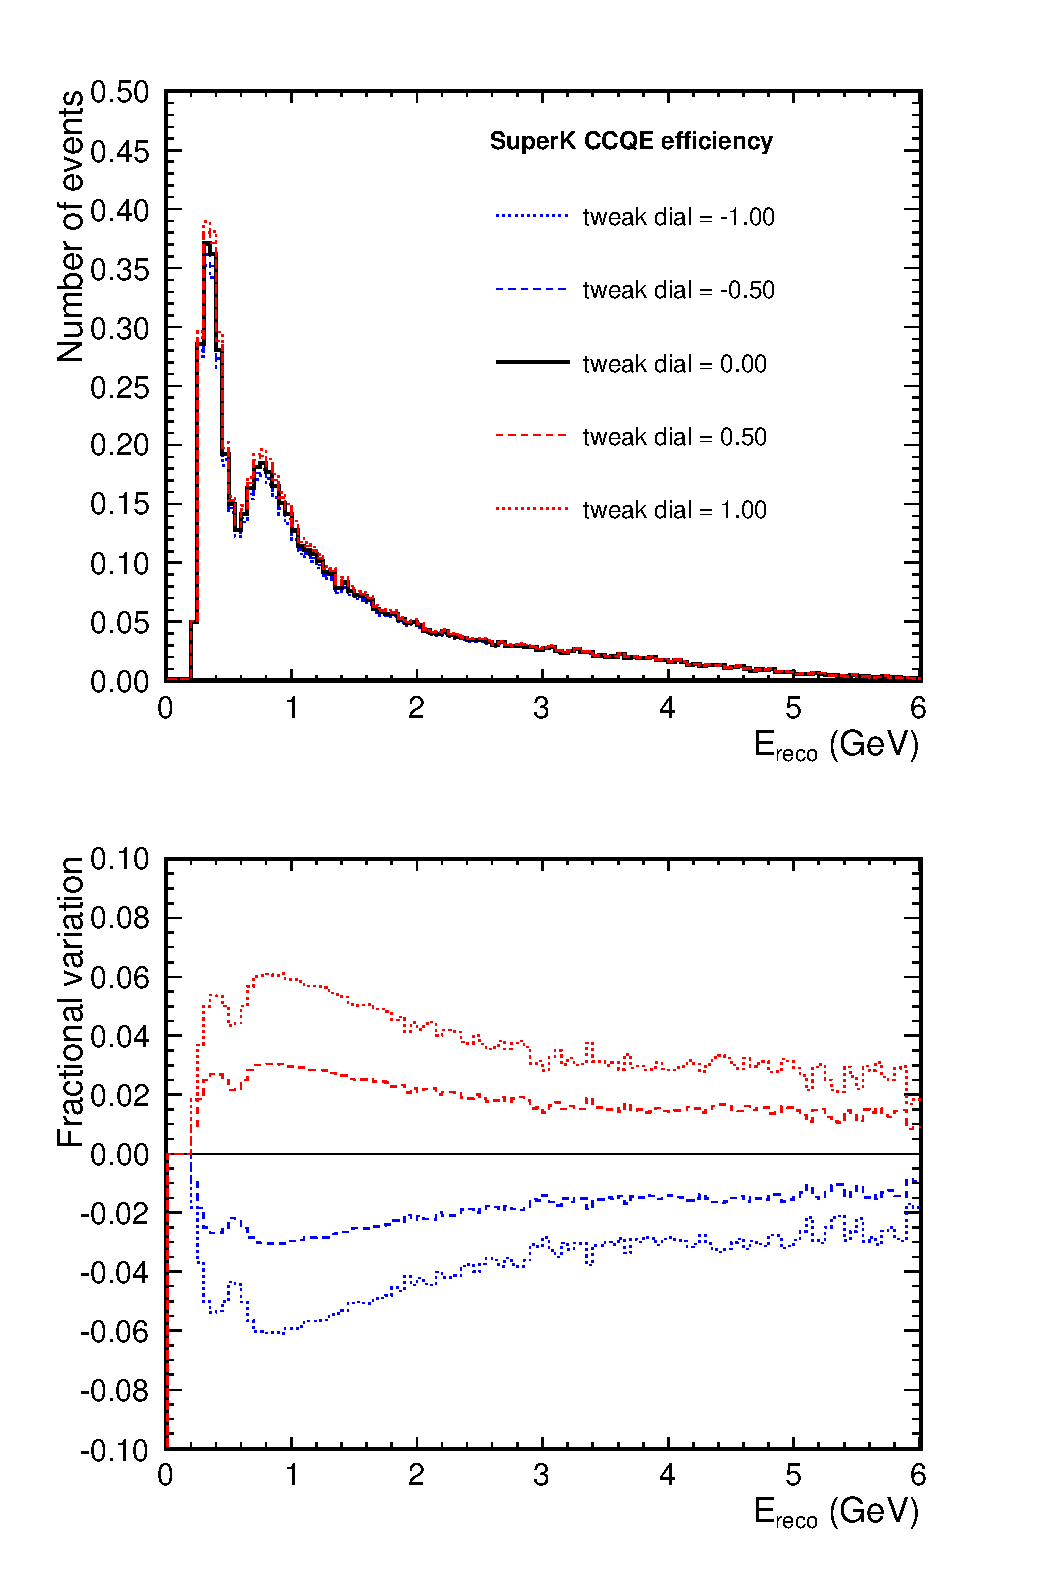
\includegraphics[width=19pc,height=21pc]{./images/predicted_spectrum/systematic_variations/genie_sk_spectrum_twk_skccqeeff_2p4Em3_1p0.eps}
\caption{
  Effect of SuperK CCQE efficiency variation to the GENIE
  reconstructed-energy spectrum of 1-ring muon-like events (after extrapolation).
  All spectra have oscillations with $sin^{2}2\theta_{23}$ = 1.0 and $\Delta m^{2}_{23}$ = 2.4$\times10^{-3}$ $eV^{2}/c^{4}$ applied.  
}
\label{fig:genie_sk_spectrum_twk_skccqeeff_2p4Em3_1p0}
\end{minipage}
\hspace{0.06\linewidth}
\begin{minipage}[t]{0.47\linewidth}
\centering
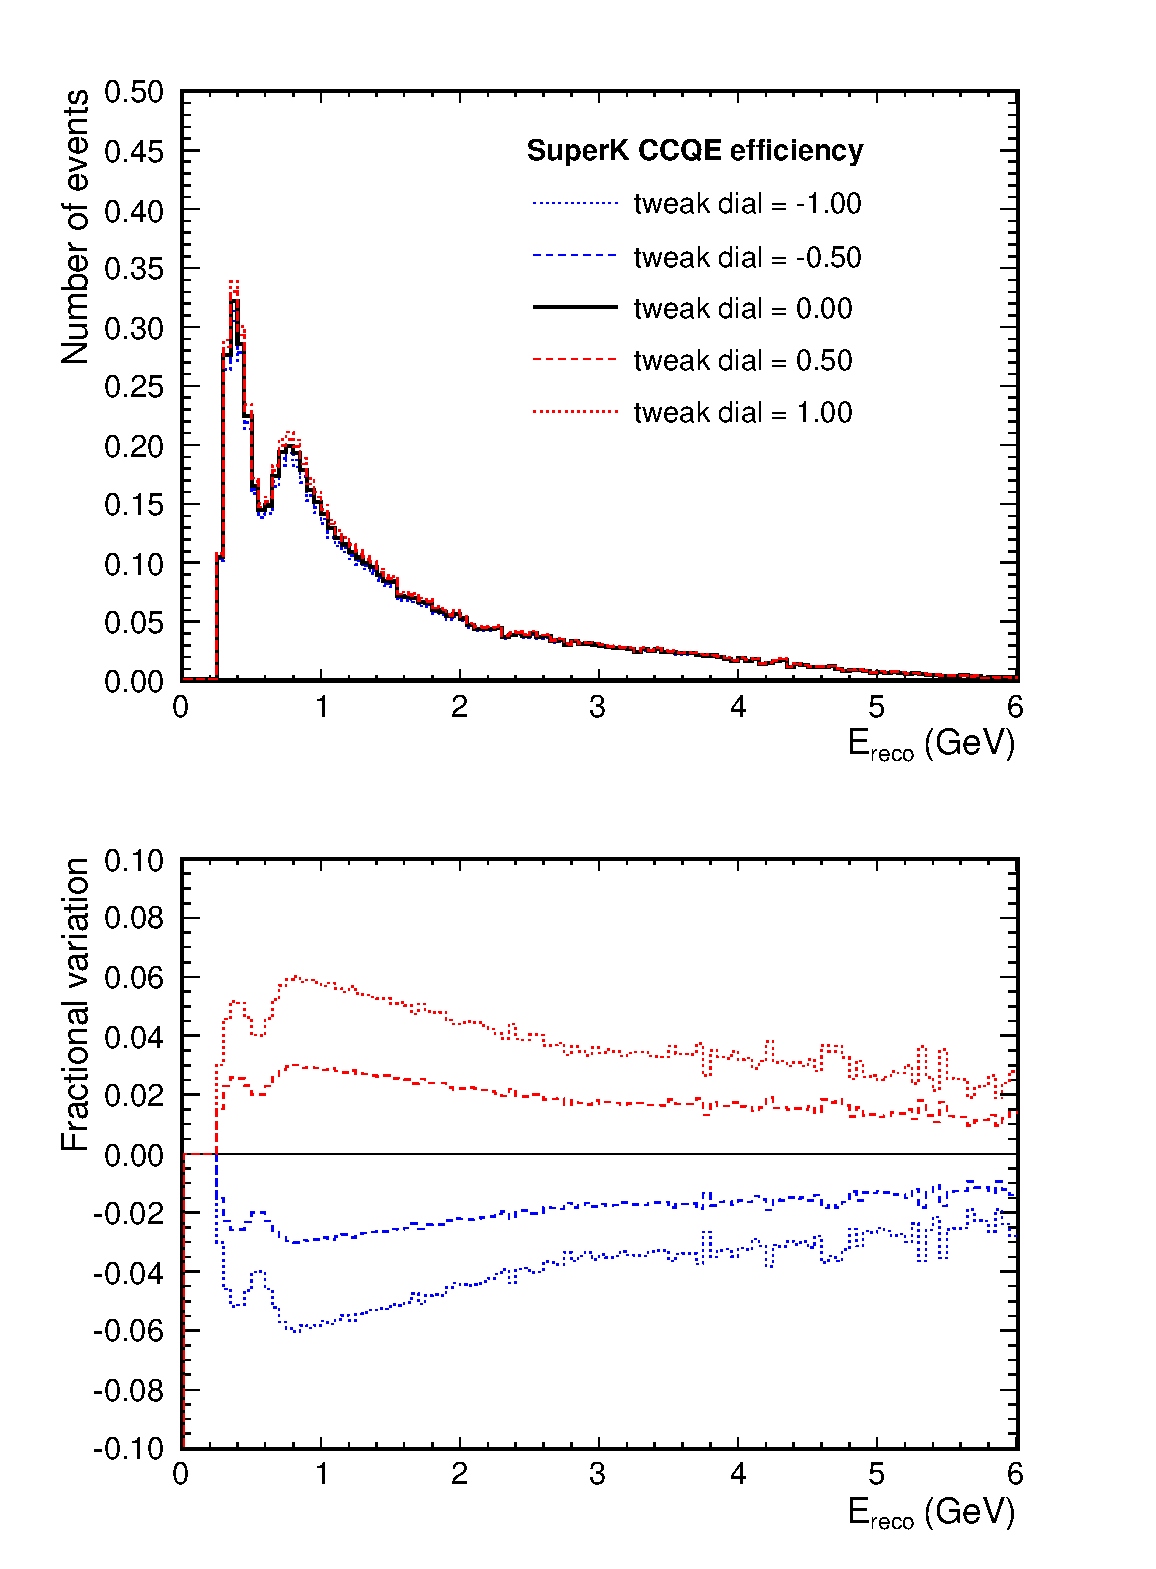
\includegraphics[width=19pc,height=21pc]{images/predicted_spectrum/systematic_variations/neut_sk_spectrum_twk_skccqeeff_2p4Em3_1p0.eps}
\caption{
  Effect of SuperK CCQE efficiency variation to the NEUT
  reconstructed-energy spectrum of 1-ring muon-like events (after extrapolation).
  All spectra have oscillations with $sin^{2}2\theta_{23}$ = 1.0 and $\Delta m^{2}_{23}$ = 2.4$\times10^{-3}$ $eV^{2}/c^{4}$ applied.  
}
\label{fig:neut_sk_spectrum_twk_skccqeeff_2p4Em3_1p0}
\end{minipage}
\end{figure}


%
% SuperK CCnonQE efficiency
%

\begin{figure}[ht]
\begin{minipage}[t]{0.47\linewidth}
\centering
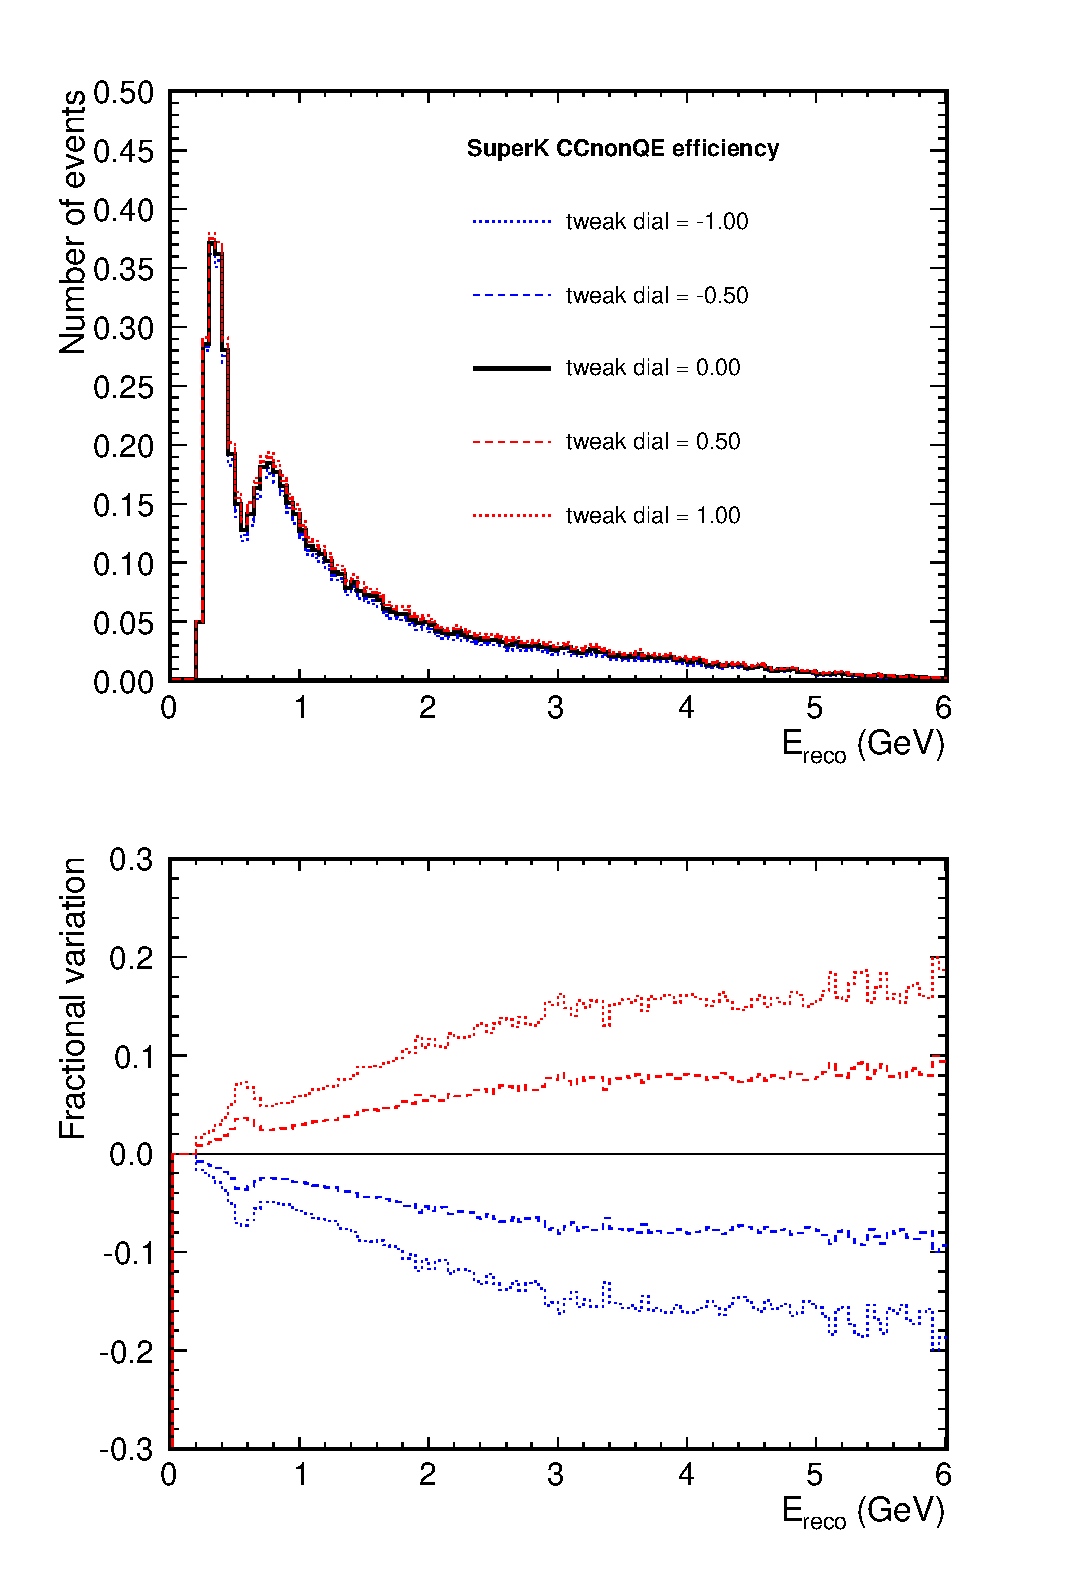
\includegraphics[width=19pc,height=21pc]{./images/predicted_spectrum/systematic_variations/genie_sk_spectrum_twk_skccnonqeeff_2p4Em3_1p0.eps}
\caption{
  Effect of SuperK CCnonQE efficiency variation to the GENIE
  reconstructed-energy spectrum of 1-ring muon-like events (after extrapolation).
  All spectra have oscillations with $sin^{2}2\theta_{23}$ = 1.0 and $\Delta m^{2}_{23}$ = 2.4$\times10^{-3}$ $eV^{2}/c^{4}$ applied.  
}
\label{fig:genie_sk_spectrum_twk_sknonccqeeff_2p4Em3_1p0}
\end{minipage}
\hspace{0.06\linewidth}
\begin{minipage}[t]{0.47\linewidth}
\centering
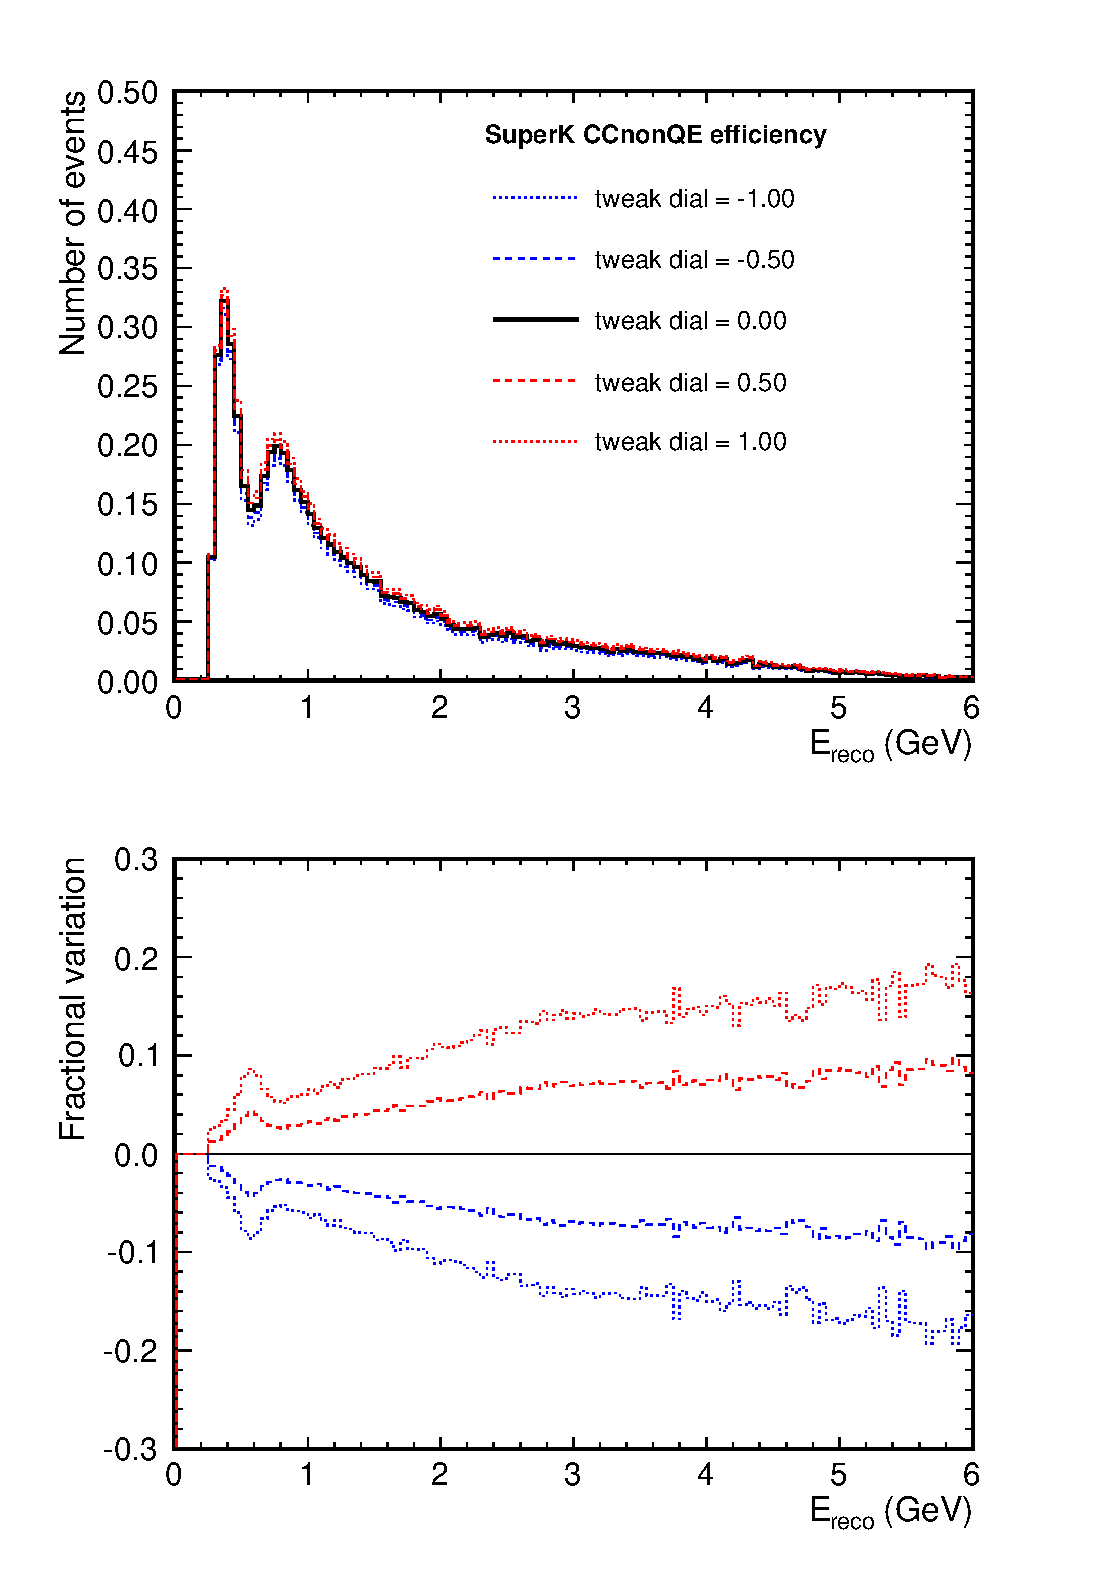
\includegraphics[width=19pc,height=21pc]{images/predicted_spectrum/systematic_variations/neut_sk_spectrum_twk_skccnonqeeff_2p4Em3_1p0.eps}
\caption{
  Effect of SuperK CCnonQE efficiency variation to the NEUT
  reconstructed-energy spectrum of 1-ring muon-like events (after extrapolation).
  All spectra have oscillations with $sin^{2}2\theta_{23}$ = 1.0 and $\Delta m^{2}_{23}$ = 2.4$\times10^{-3}$ $eV^{2}/c^{4}$ applied.  
}
\label{fig:neut_sk_spectrum_twk_skccnonqeeff_2p4Em3_1p0}
\end{minipage}
\end{figure}

%
% SuperK NC efficiency
%

\begin{figure}[ht]
\begin{minipage}[t]{0.47\linewidth}
\centering
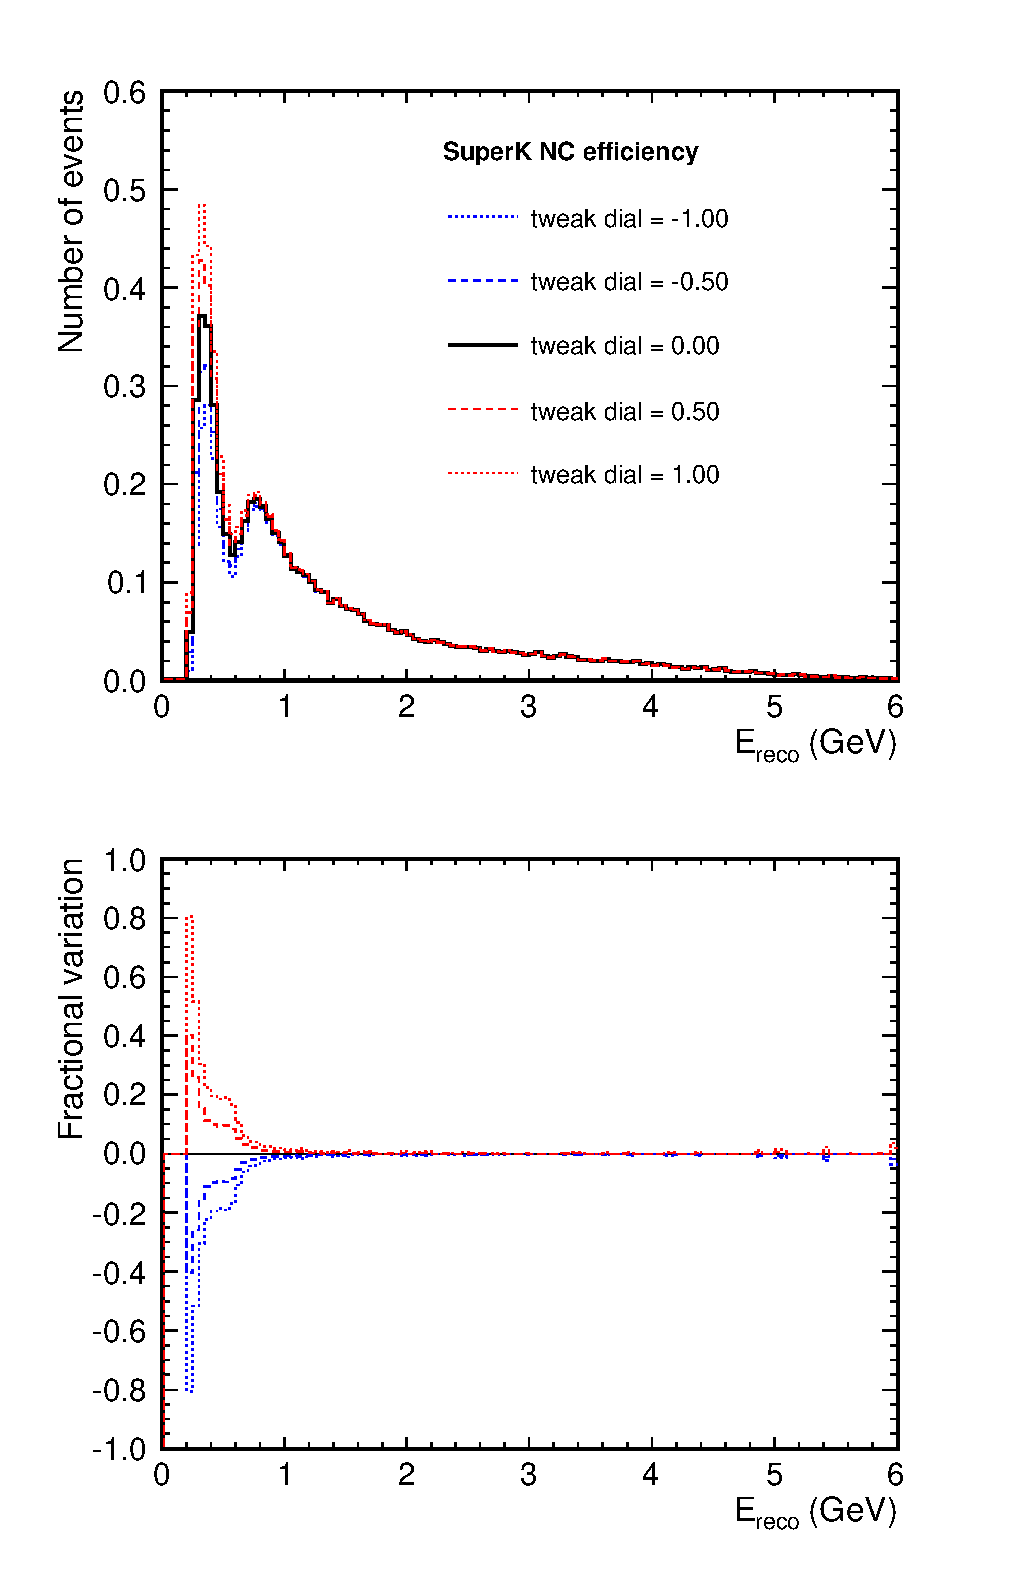
\includegraphics[width=19pc,height=21pc]{./images/predicted_spectrum/systematic_variations/genie_sk_spectrum_twk_sknceff_2p4Em3_1p0.eps}
\caption{
  Effect of SuperK NC efficiency variation to the GENIE
  reconstructed-energy spectrum of 1-ring muon-like events (after extrapolation).
  All spectra have oscillations with $sin^{2}2\theta_{23}$ = 1.0 and $\Delta m^{2}_{23}$ = 2.4$\times10^{-3}$ $eV^{2}/c^{4}$ applied.  
}
\label{fig:genie_sk_spectrum_twk_sknceff_2p4Em3_1p0}
\end{minipage}
\hspace{0.06\linewidth}
\begin{minipage}[t]{0.47\linewidth}
\centering
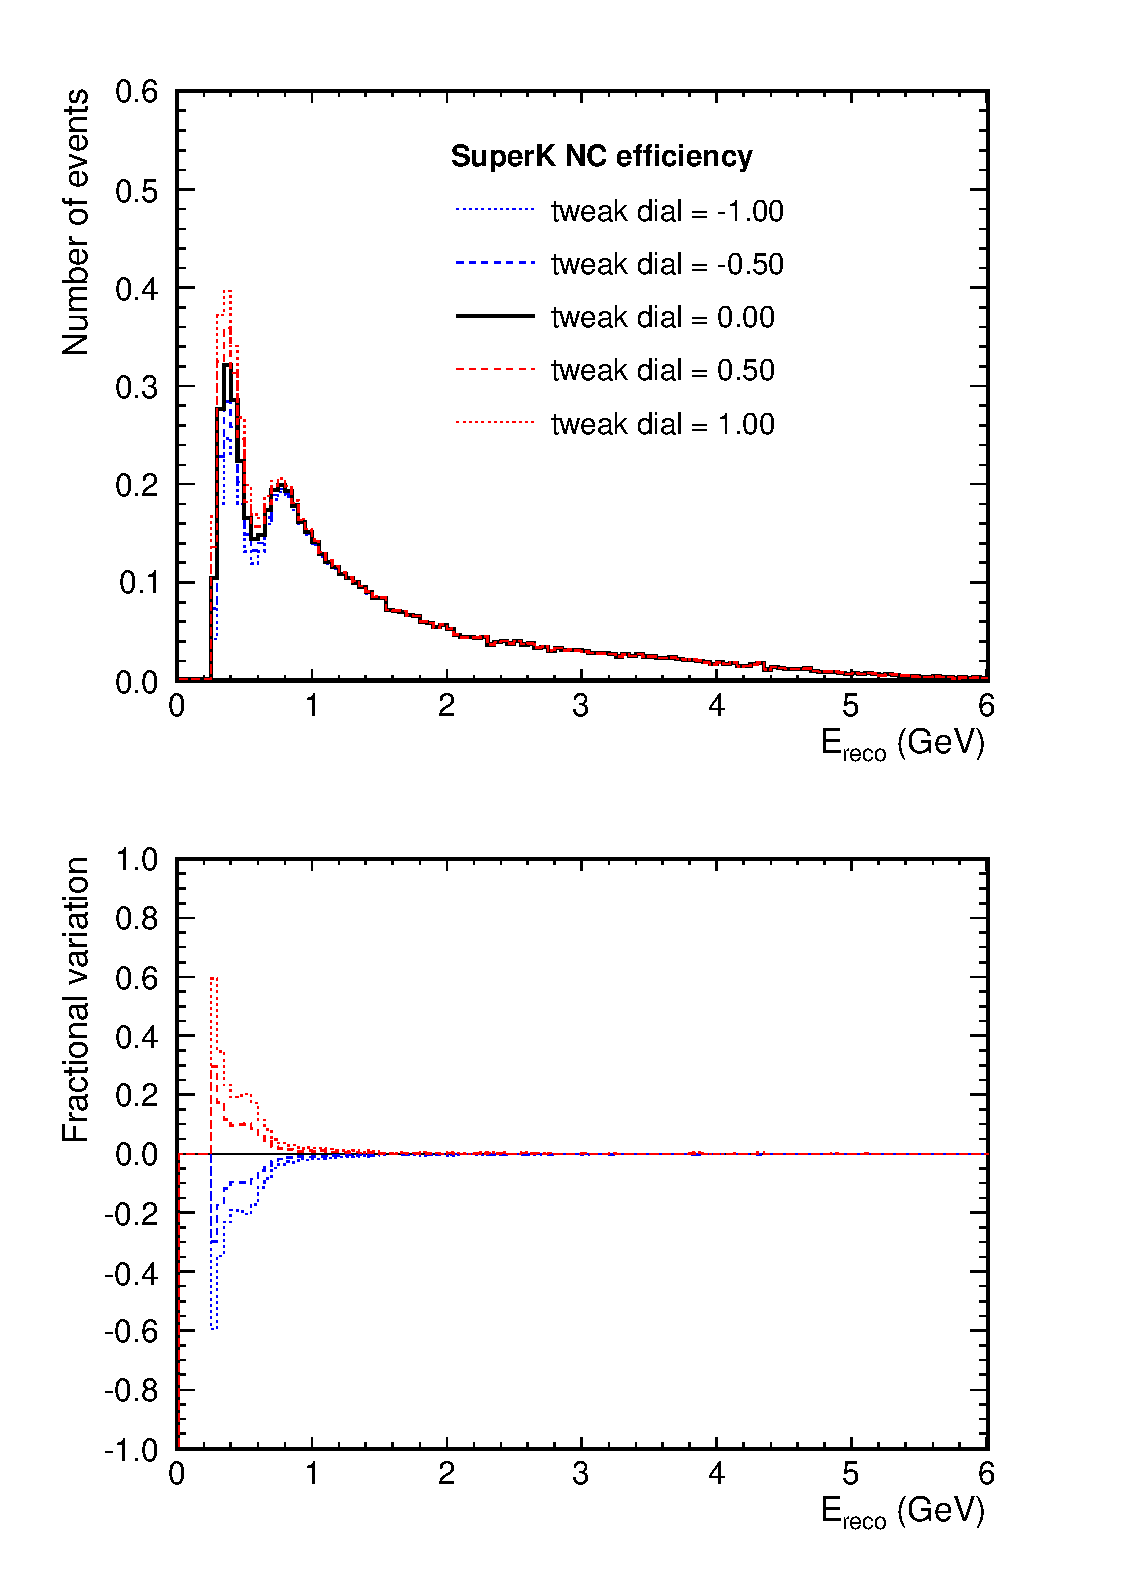
\includegraphics[width=19pc,height=21pc]{images/predicted_spectrum/systematic_variations/neut_sk_spectrum_twk_sknceff_2p4Em3_1p0.eps}
\caption{
  Effect of SuperK NC efficiency variation to the NEUT
  reconstructed-energy spectrum of 1-ring muon-like events (after extrapolation).
  All spectra have oscillations with $sin^{2}2\theta_{23}$ = 1.0 and $\Delta m^{2}_{23}$ = 2.4$\times10^{-3}$ $eV^{2}/c^{4}$ applied.  
}
\label{fig:neut_sk_spectrum_twk_sknceff_2p4Em3_1p0}
\end{minipage}
\end{figure}


%
% SuperK nue CC efficiency
%

\begin{figure}[ht]
\begin{minipage}[t]{0.47\linewidth}
\centering
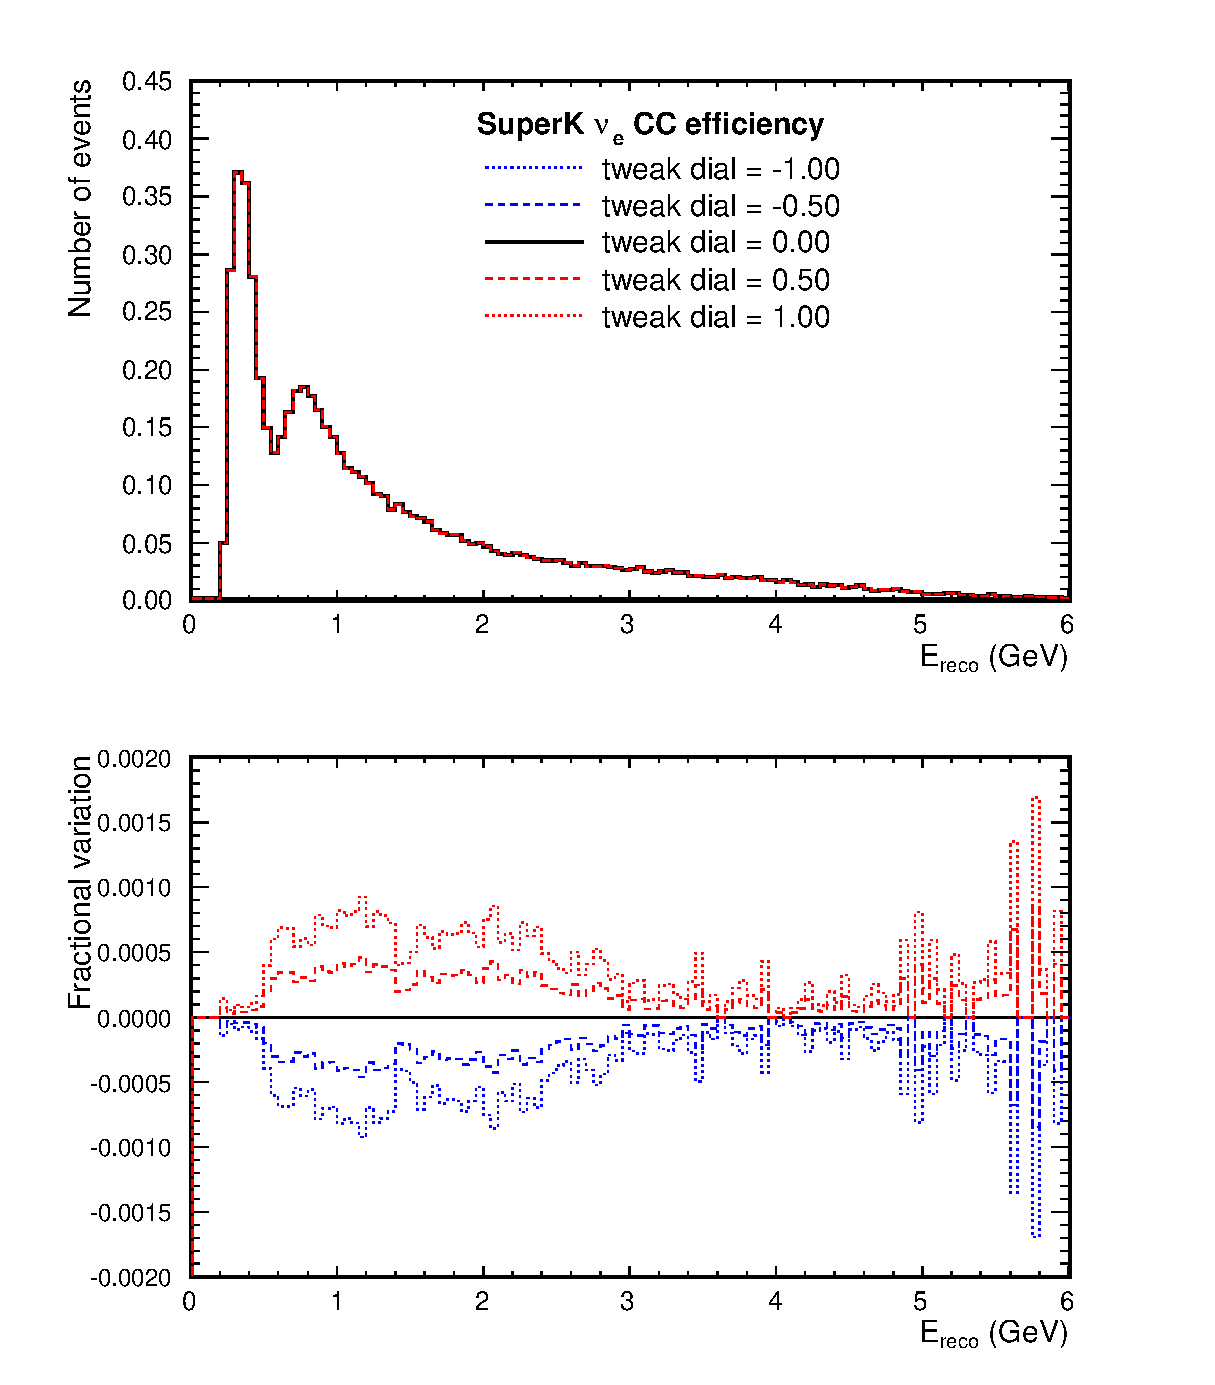
\includegraphics[width=19pc,height=21pc]{./images/predicted_spectrum/systematic_variations/genie_sk_spectrum_twk_sknuecceff_2p4Em3_1p0.eps}
\caption{
  Effect of SuperK $\nu_{e}$ CC efficiency variation to the GENIE
  reconstructed-energy spectrum of 1-ring muon-like events (after extrapolation).
  All spectra have oscillations with $sin^{2}2\theta_{23}$ = 1.0 and $\Delta m^{2}_{23}$ = 2.4$\times10^{-3}$ $eV^{2}/c^{4}$ applied.  
}
\label{fig:genie_sk_spectrum_twk_sknuecceff_2p4Em3_1p0}
\end{minipage}
\hspace{0.06\linewidth}
\begin{minipage}[t]{0.47\linewidth}
\centering
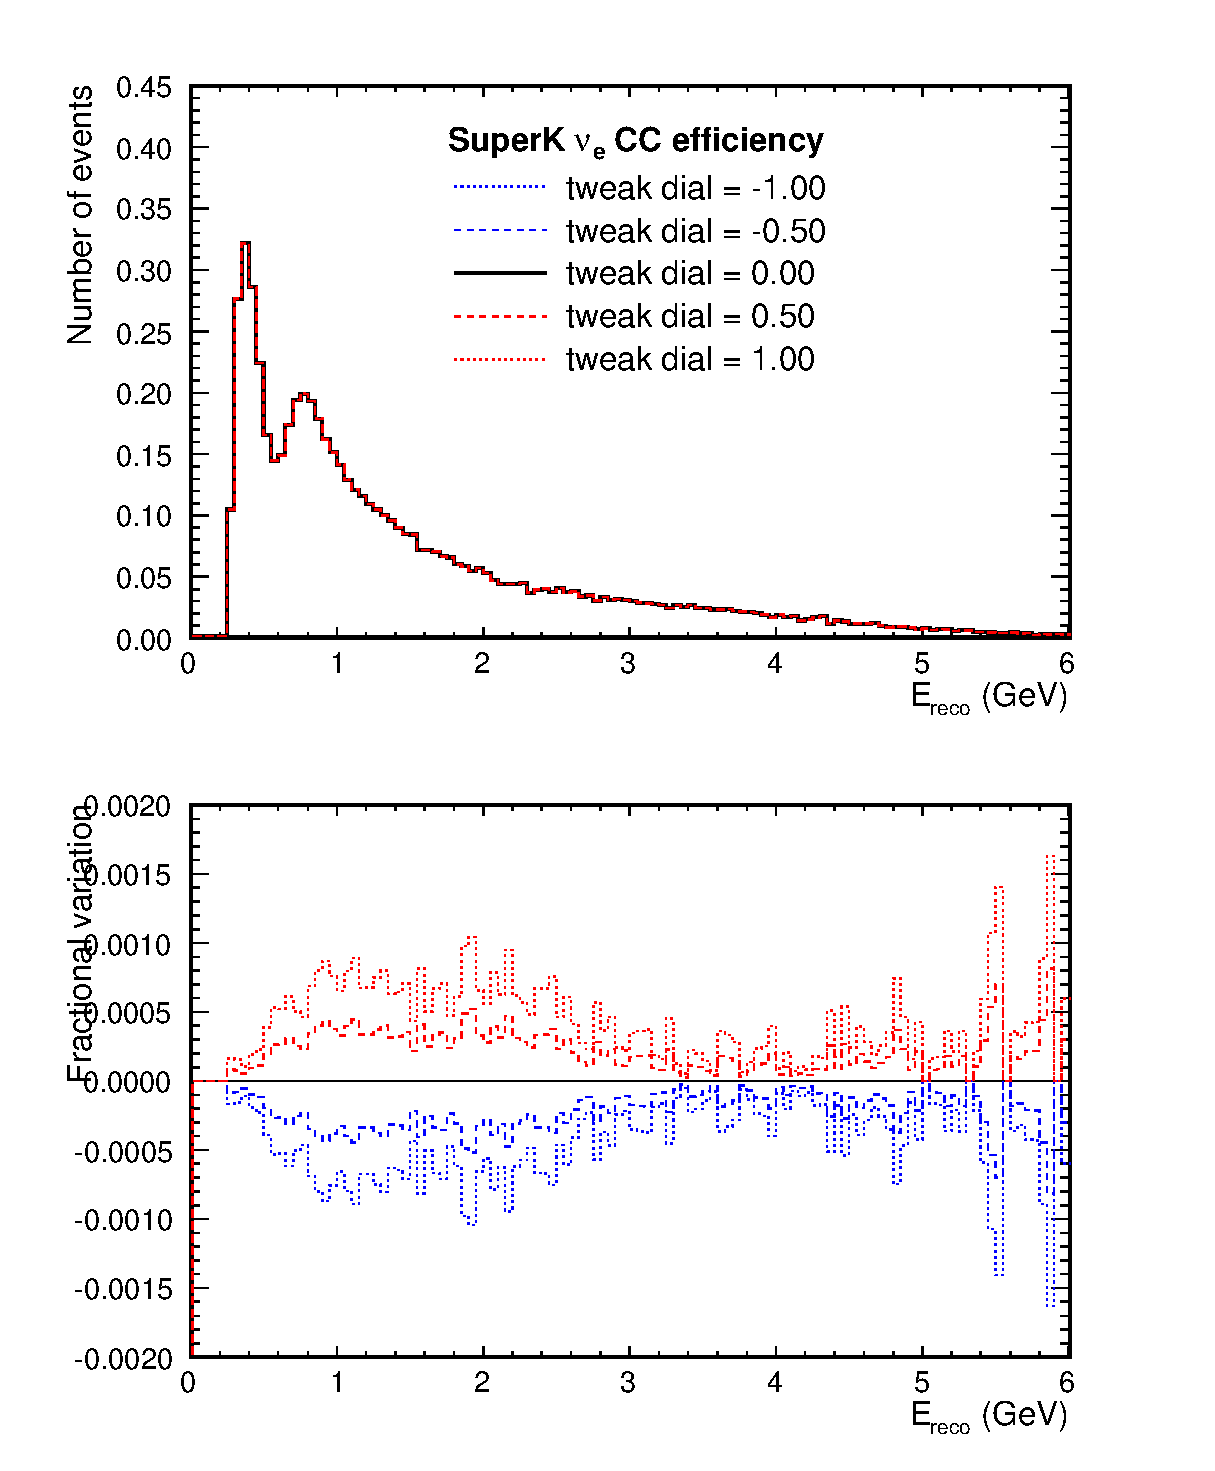
\includegraphics[width=19pc,height=21pc]{images/predicted_spectrum/systematic_variations/neut_sk_spectrum_twk_sknuecceff_2p4Em3_1p0.eps}
\caption{
  Effect of SuperK $\nu_{e}$ CC efficiency variation to the NEUT
  reconstructed-energy spectrum of 1-ring muon-like events (after extrapolation).
  All spectra have oscillations with $sin^{2}2\theta_{23}$ = 1.0 and $\Delta m^{2}_{23}$ = 2.4$\times10^{-3}$ $eV^{2}/c^{4}$ applied.  
}
\label{fig:neut_sk_spectrum_twk_sknuecceff_2p4Em3_1p0}
\end{minipage}
\end{figure}


%
% SuperK energy scale
%

\begin{figure}[ht]
\begin{minipage}[t]{0.47\linewidth}
\centering
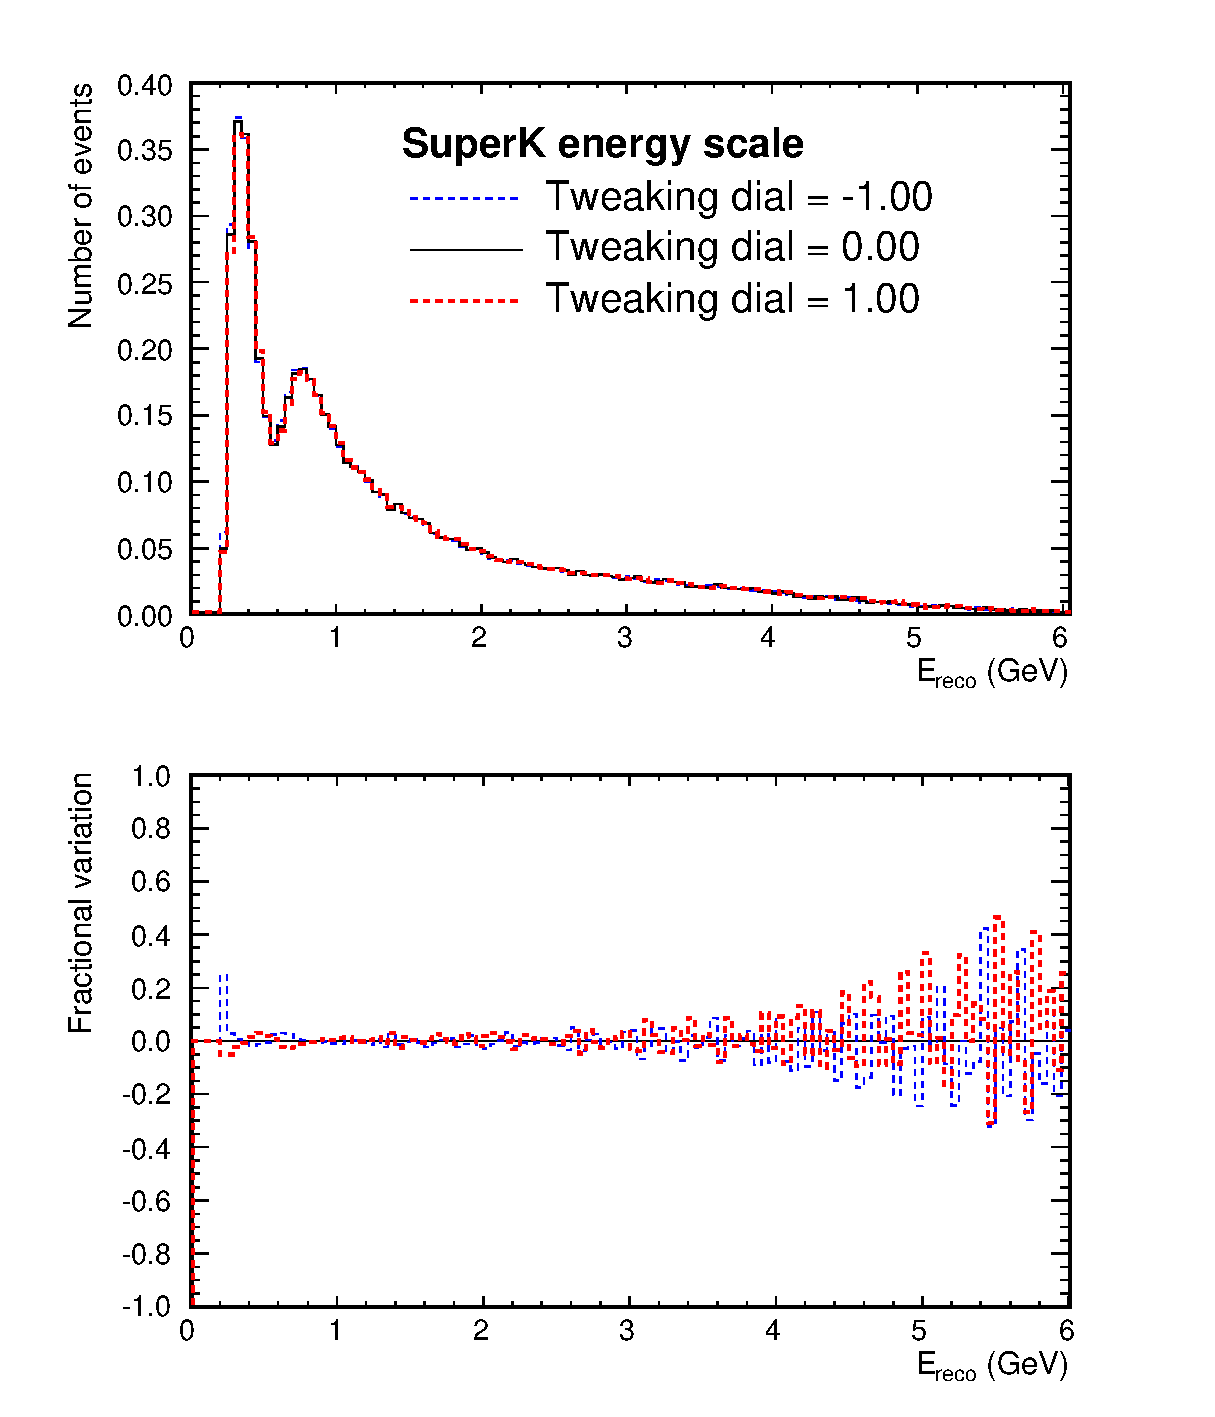
\includegraphics[width=19pc,height=21pc]{./images/predicted_spectrum/systematic_variations/genie_sk_spectrum_twk_skescale_2p4Em3_1p0.eps}
\caption{
  Effect of SuperK energy scale variation to the GENIE
  reconstructed-energy spectrum of 1-ring muon-like events (after extrapolation).
  All spectra have oscillations with $sin^{2}2\theta_{23}$ = 1.0 and $\Delta m^{2}_{23}$ = 2.4$\times10^{-3}$ $eV^{2}/c^{4}$ applied.  
}
\label{fig:genie_sk_spectrum_twk_skescale_2p4Em3_1p0}
\end{minipage}
\hspace{0.06\linewidth}
\begin{minipage}[t]{0.47\linewidth}
\centering
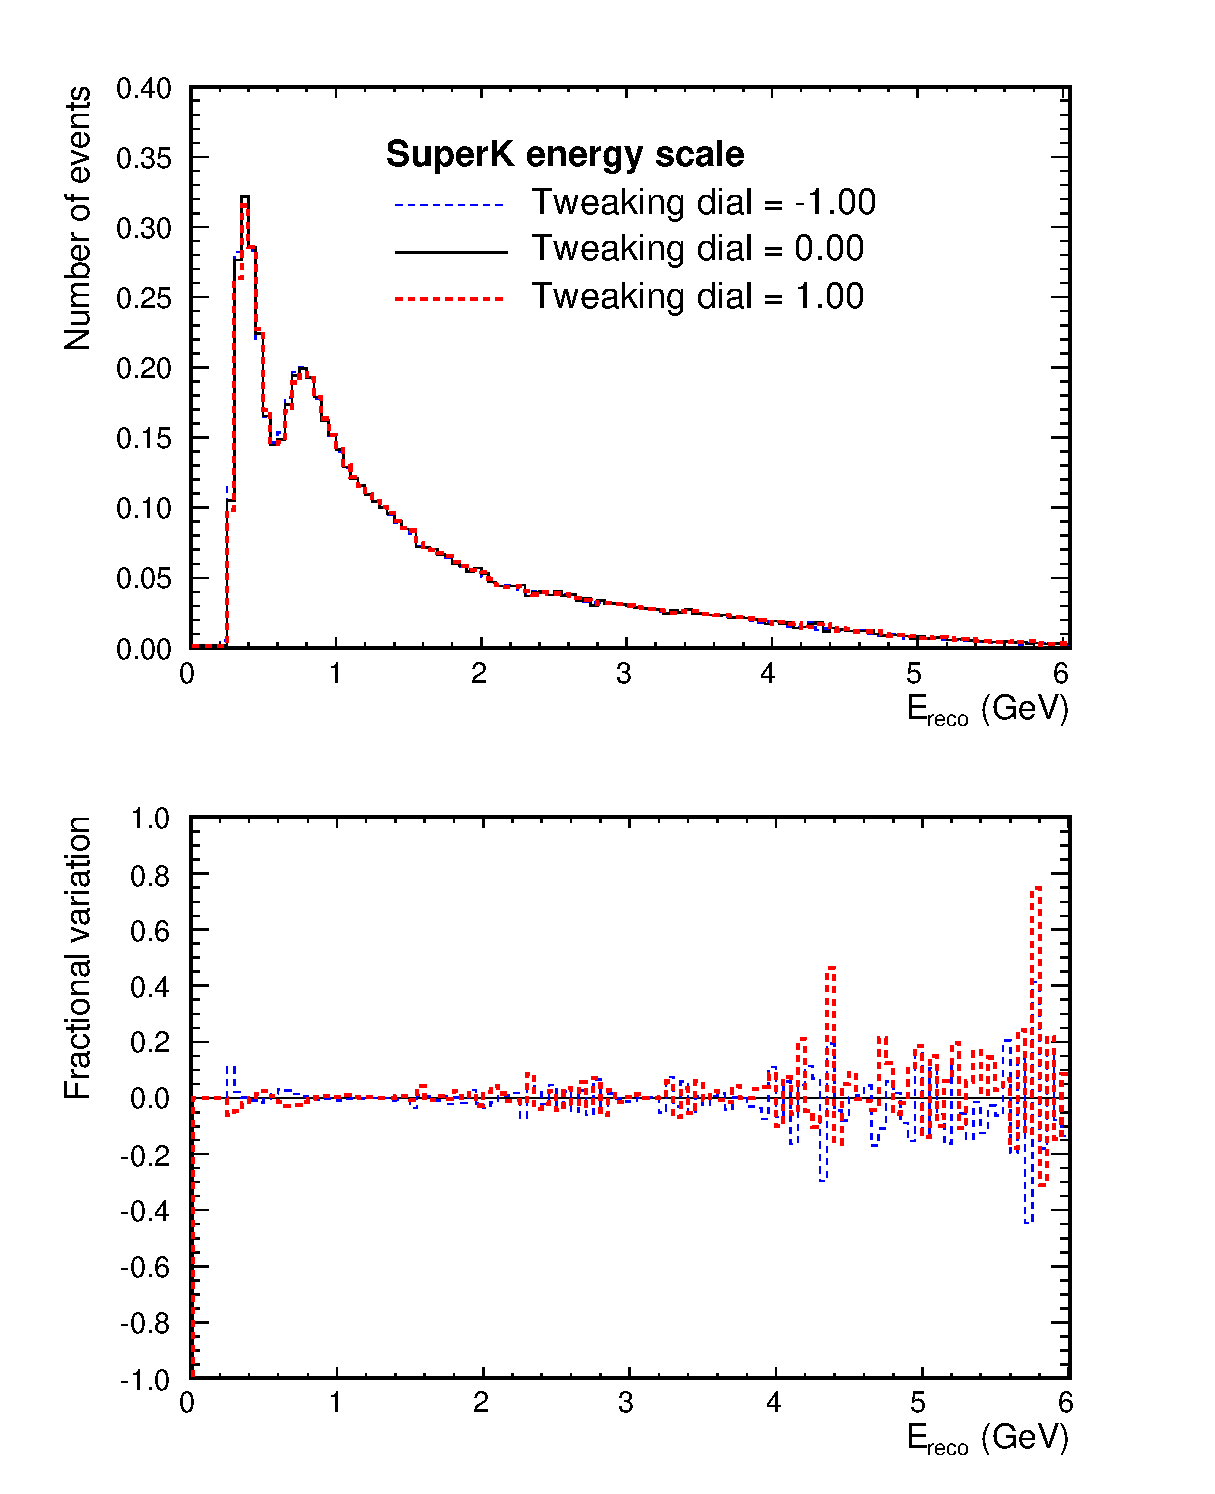
\includegraphics[width=19pc,height=21pc]{images/predicted_spectrum/systematic_variations/neut_sk_spectrum_twk_skescale_2p4Em3_1p0.eps}
\caption{
  Effect of SuperK energy scale variation to the NEUT
  reconstructed-energy spectrum of 1-ring muon-like events (after extrapolation).
  All spectra have oscillations with $sin^{2}2\theta_{23}$ = 1.0 and $\Delta m^{2}_{23}$ = 2.4$\times10^{-3}$ $eV^{2}/c^{4}$ applied.  
}
\label{fig:neut_sk_spectrum_twk_skescale_2p4Em3_1p0}
\end{minipage}
\end{figure}

%
% nd280 efficiency
%

\begin{figure}[ht]
\begin{minipage}[t]{0.47\linewidth}
\centering
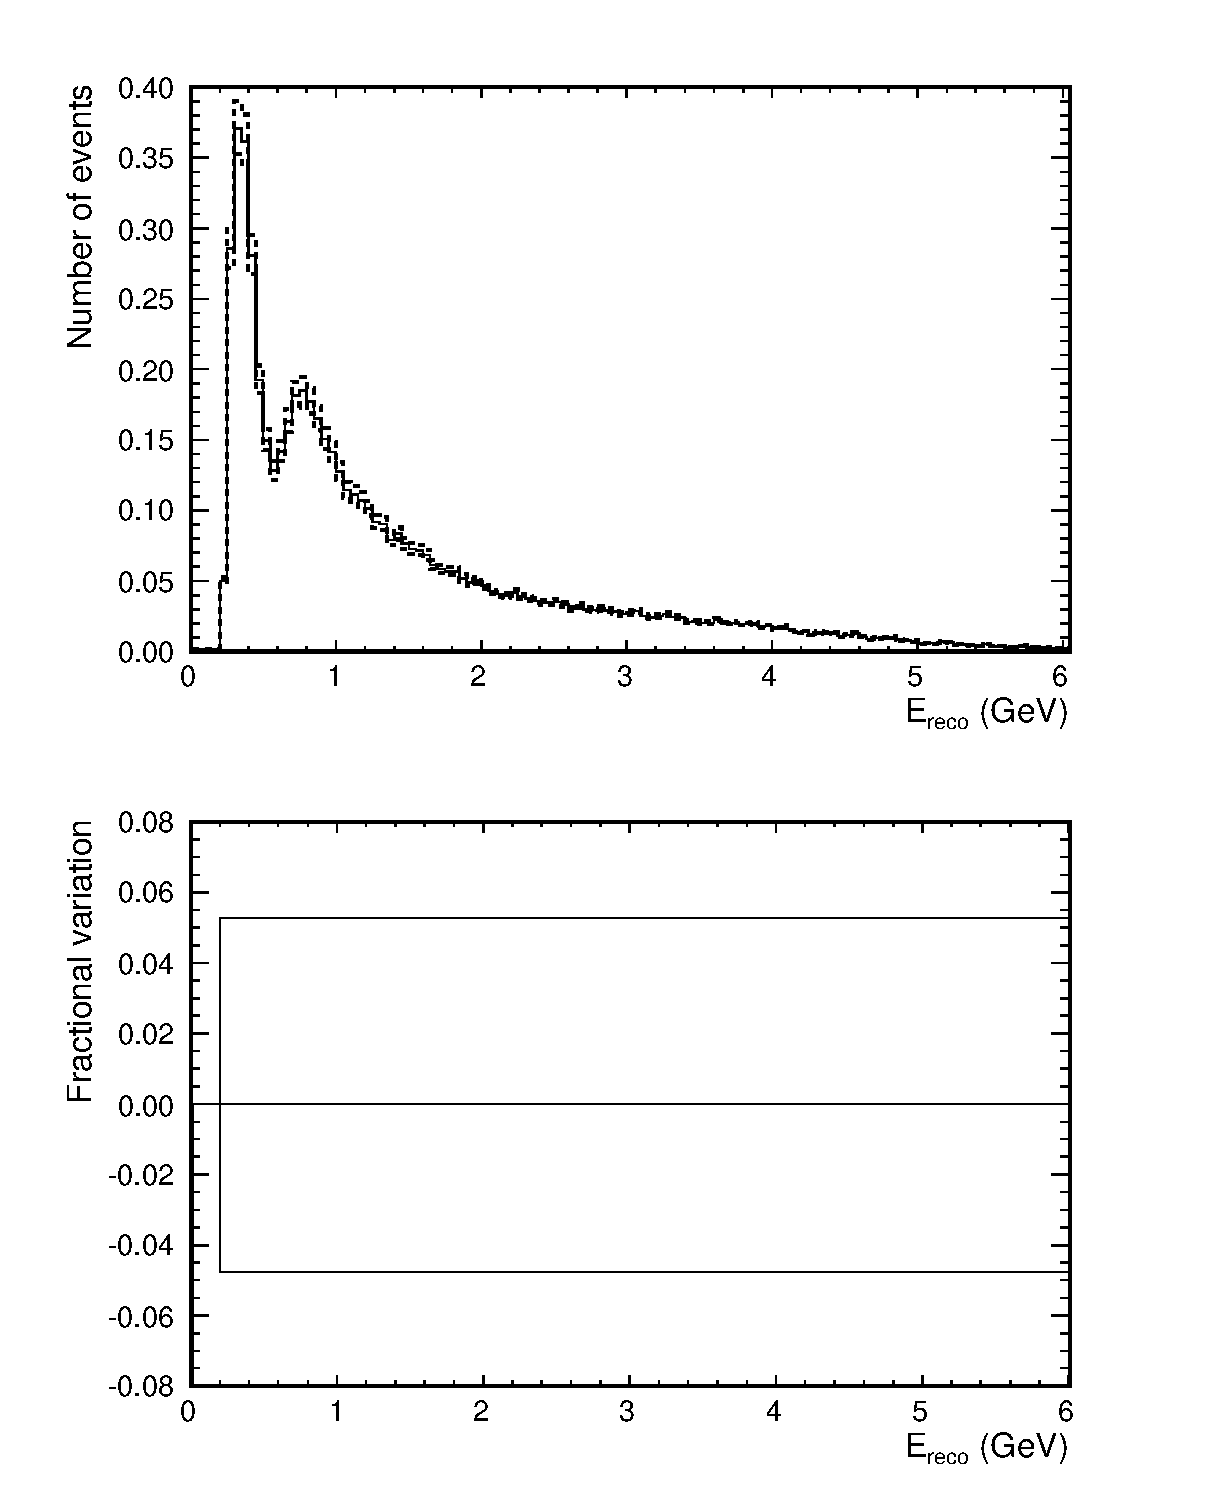
\includegraphics[width=19pc,height=21pc]{./images/predicted_spectrum/systematic_variations/genie_sk_spectrum_twk_nd280eff_2p4Em3_1p0.eps}
\caption{
  Effect of ND280 efficiency variation to the GENIE
  reconstructed-energy spectrum of 1-ring muon-like events (after extrapolation).
  All spectra have oscillations with $sin^{2}2\theta_{23}$ = 1.0 and $\Delta m^{2}_{23}$ = 2.4$\times10^{-3}$ $eV^{2}/c^{4}$ applied.  
}
\label{fig:genie_sk_spectrum_twk_nd280eff_2p4Em3_1p0}
\end{minipage}
\hspace{0.06\linewidth}
\begin{minipage}[t]{0.47\linewidth}
\centering
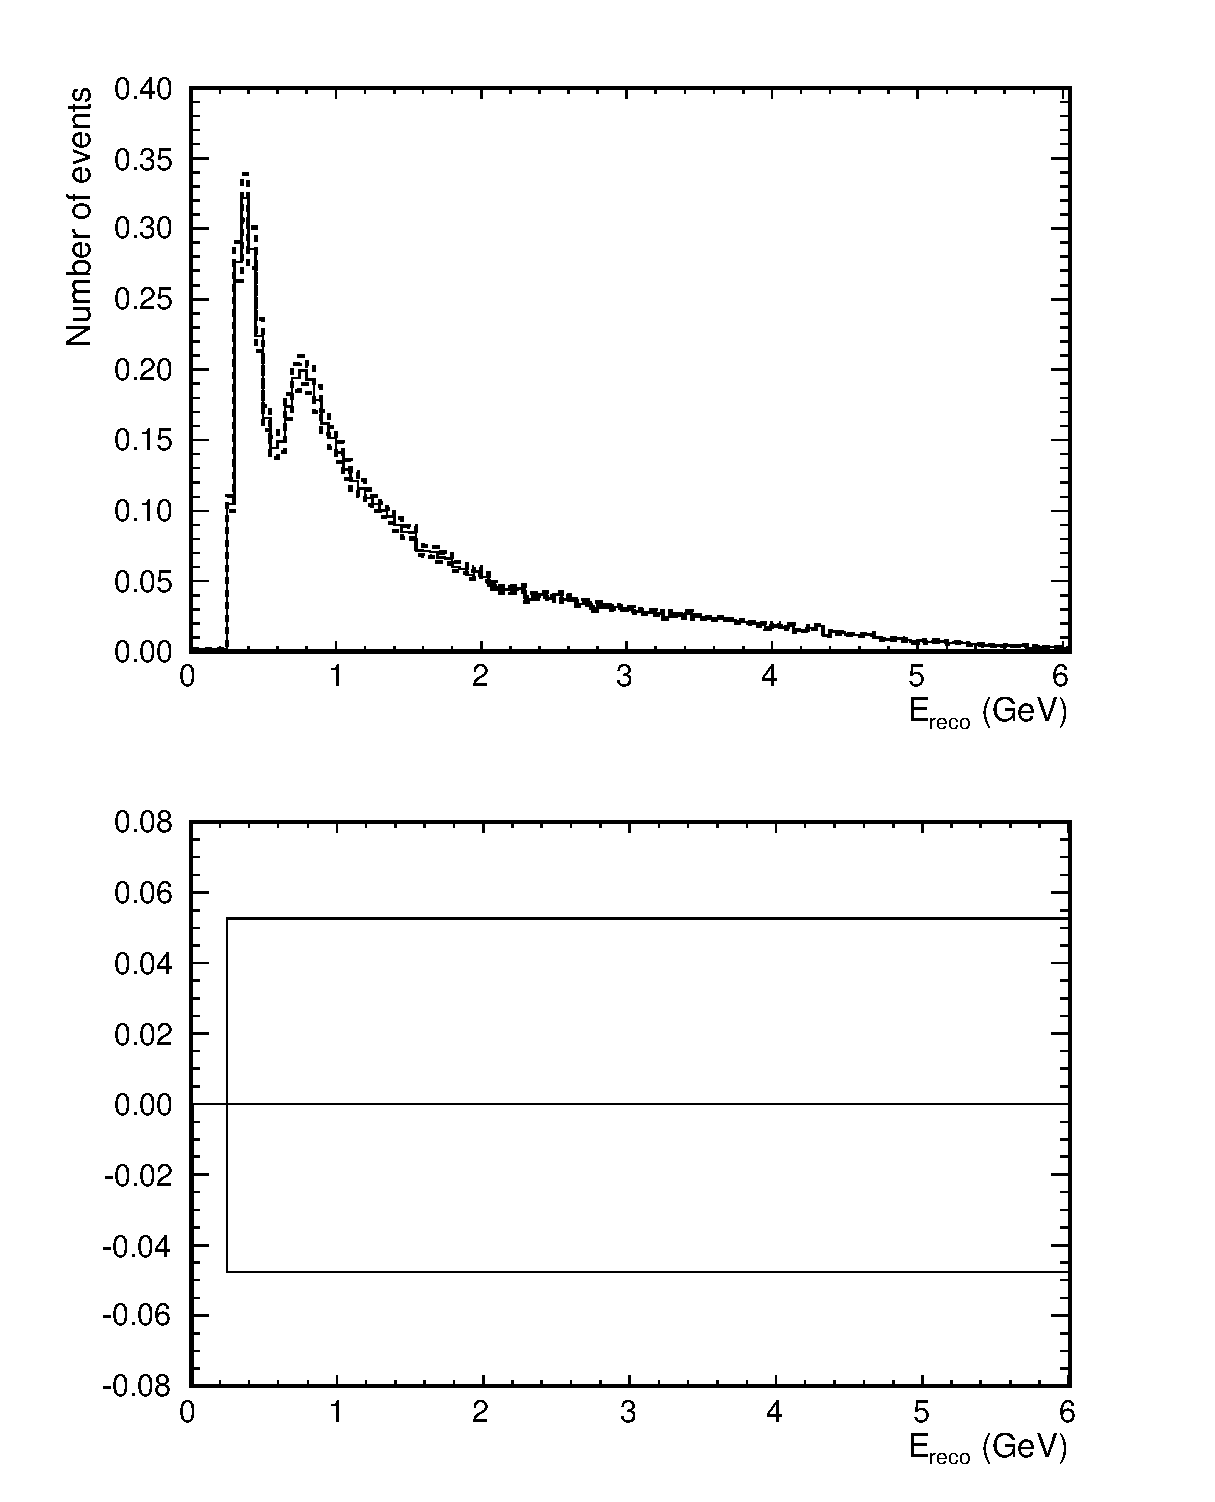
\includegraphics[width=19pc,height=21pc]{images/predicted_spectrum/systematic_variations/neut_sk_spectrum_twk_nd280eff_2p4Em3_1p0.eps}
\caption{
  Effect of ND280 efficiency variation to the NEUT
  reconstructed-energy spectrum of 1-ring muon-like events (after extrapolation).
  All spectra have oscillations with $sin^{2}2\theta_{23}$ = 1.0 and $\Delta m^{2}_{23}$ = 2.4$\times10^{-3}$ $eV^{2}/c^{4}$ applied.  
}
\label{fig:neut_sk_spectrum_twk_nd280eff_2p4Em3_1p0}
\end{minipage}
\end{figure}


%
% Beam norm
%

\begin{figure}[ht]
\begin{minipage}[t]{0.47\linewidth}
\centering
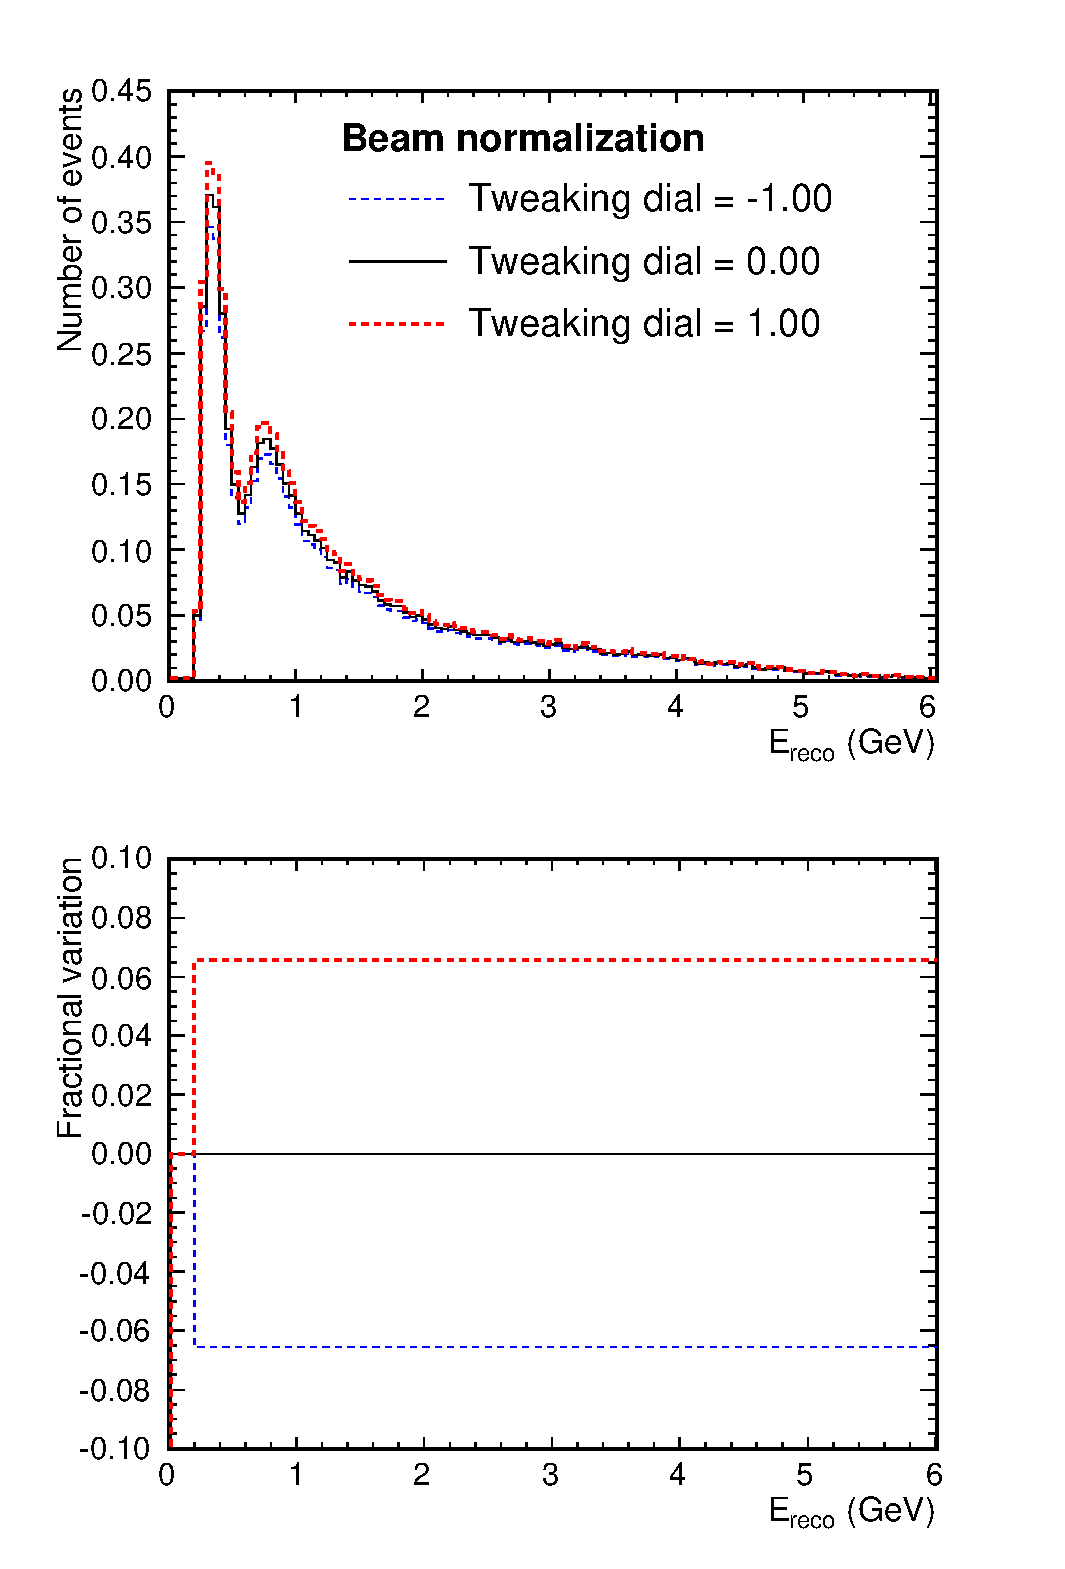
\includegraphics[width=17pc,height=17pc]{./images/predicted_spectrum/systematic_variations/genie_sk_spectrum_twk_bnorm_2p4Em3_1p0.eps}
\caption{
  Effect of beam normalization variation to the GENIE
  reconstructed-energy spectrum of 1-ring muon-like events (after extrapolation).
  All spectra have oscillations with $sin^{2}2\theta_{23}$ = 1.0 and $\Delta m^{2}_{23}$ = 2.4$\times10^{-3}$ $eV^{2}/c^{4}$ applied.  
}
\label{fig:genie_sk_spectrum_twk_bnorm_2p4Em3_1p0}
\end{minipage}
\hspace{0.06\linewidth}
\begin{minipage}[t]{0.47\linewidth}
\centering
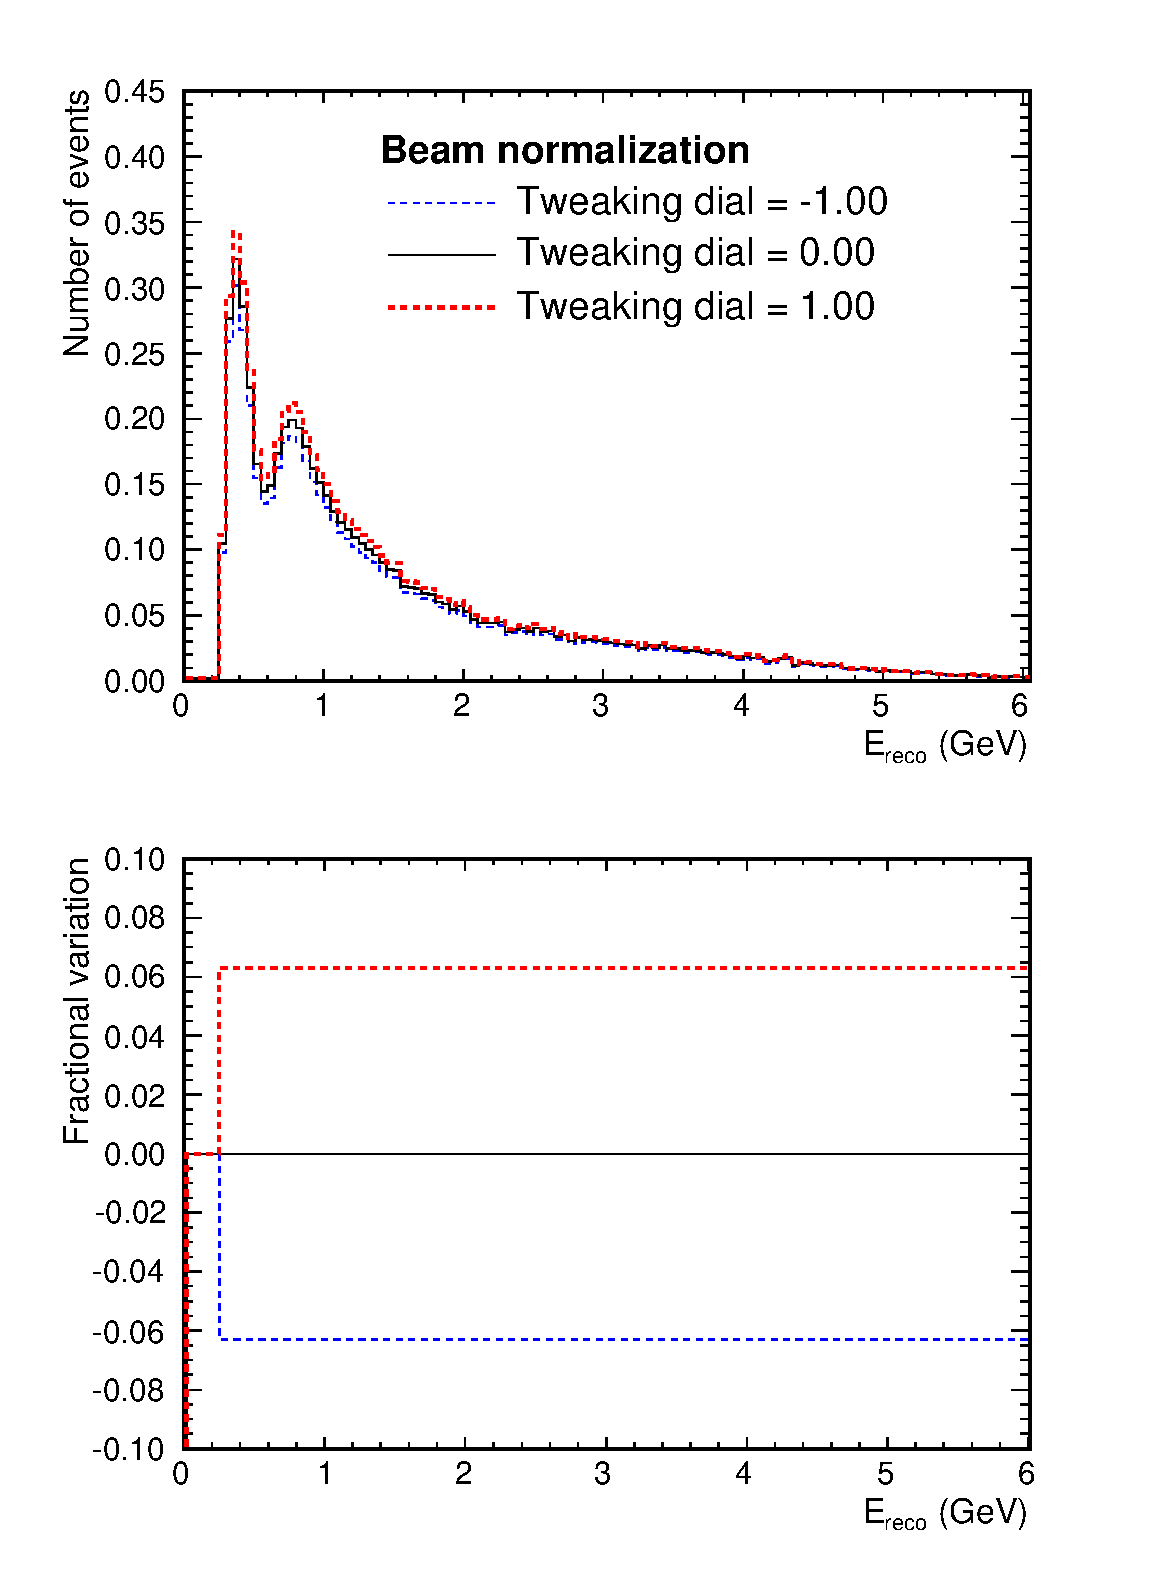
\includegraphics[width=17pc,height=17pc]{images/predicted_spectrum/systematic_variations/neut_sk_spectrum_twk_bnorm_2p4Em3_1p0.eps}
\caption{
  Effect of beam normalization variation to the NEUT
  reconstructed-energy spectrum of 1-ring muon-like events (after extrapolation).
  All spectra have oscillations with $sin^{2}2\theta_{23}$ = 1.0 and $\Delta m^{2}_{23}$ = 2.4$\times10^{-3}$ $eV^{2}/c^{4}$ applied.  
}
\label{fig:neut_sk_spectrum_twk_bnorm_2p4Em3_1p0}
\end{minipage}
\end{figure}

%
% Beam shape
%

\begin{figure}[ht]
\begin{minipage}[t]{0.47\linewidth}
\centering
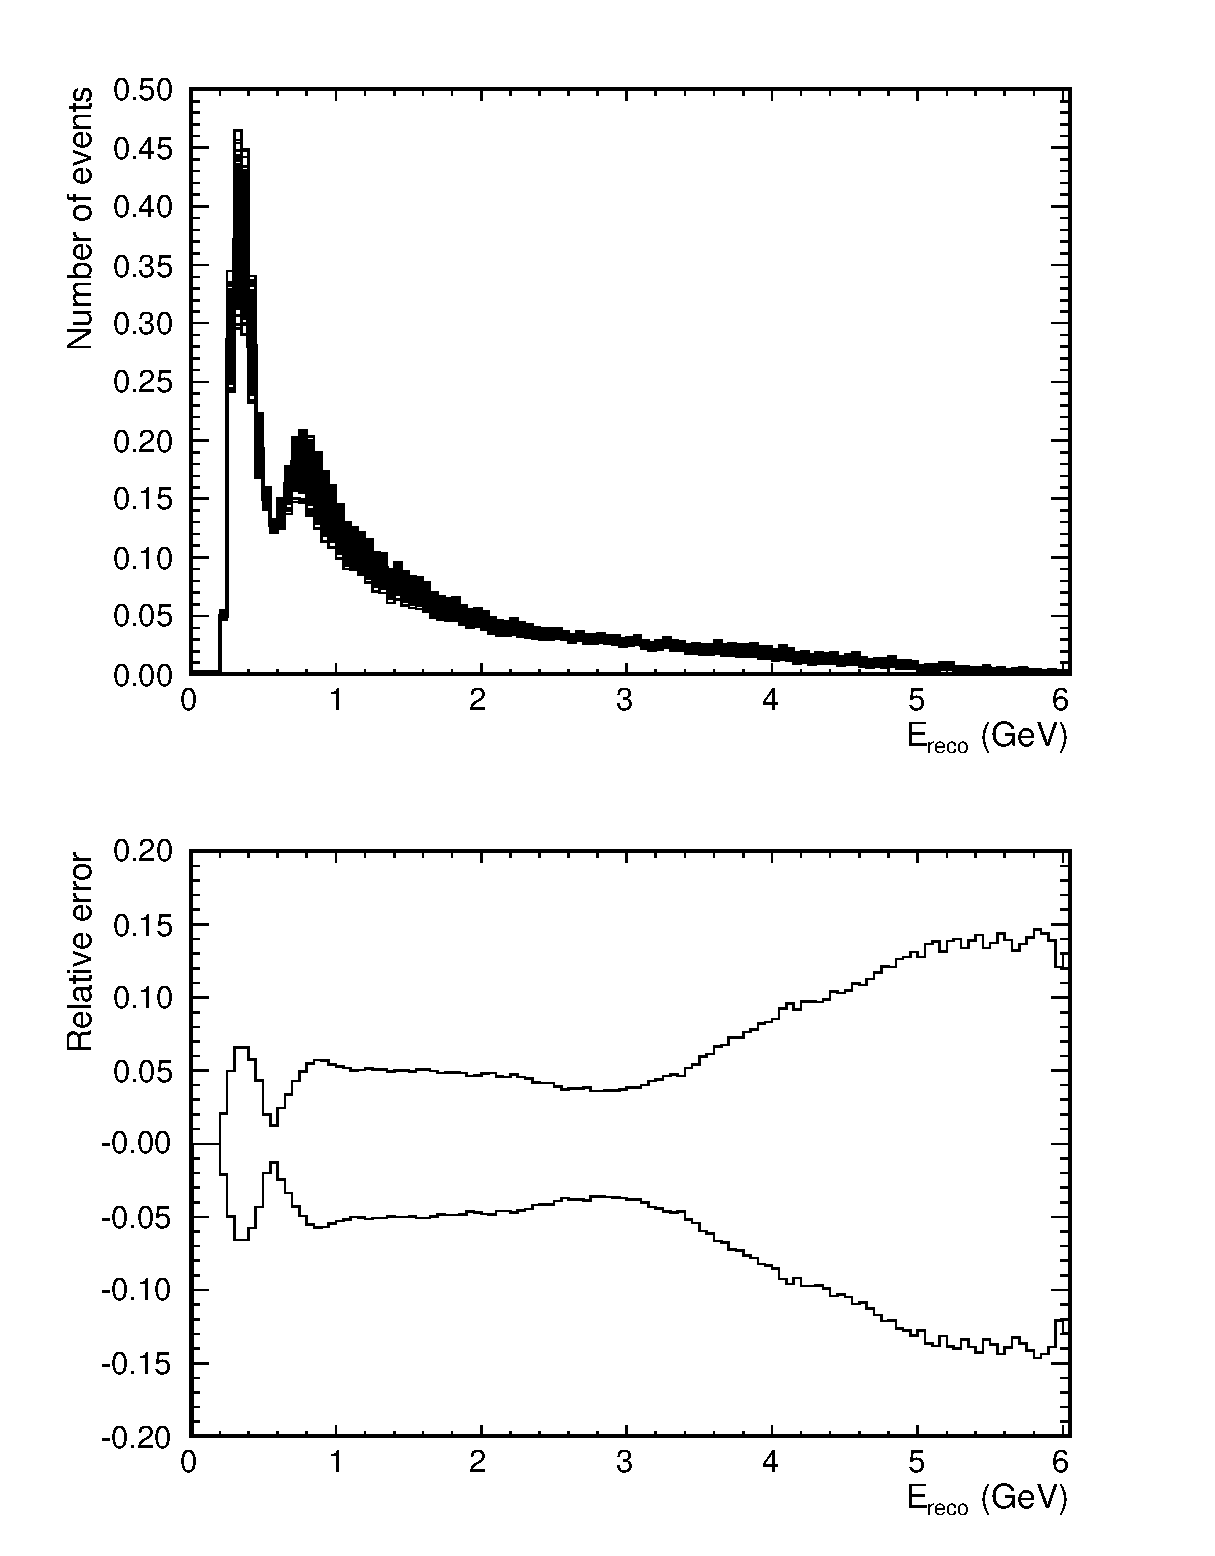
\includegraphics[width=19pc,height=19pc]{./images/predicted_spectrum/systematic_variations/genie_sk_spectrum_twk_bshape_2p4Em3_1p0.eps}
\caption{
  Effect of beam shape systematic variation to the GENIE
  reconstructed-energy spectrum of 1-ring muon-like events (after extrapolation).
  The top plot shows 2000 reconstructed-energy spectra corresponding 
  to 2000 fluxes generated using the Cholesky method (see Sec. \ref{sec:cholesky}).
  All spectra have oscillations with $sin^{2}2\theta_{23}$ = 1.0 and $\Delta m^{2}_{23}$ = 2.4$\times10^{-3}$ $eV^{2}/c^{4}$ applied
  and they are normalized to the number of events predicted using the nominal flux.
  The relative error shown in the bottom plot is calculated from the standard deviation of the randomly generated spectra.
}
\label{fig:genie_sk_spectrum_twk_bshape_2p4Em3_1p0}
\end{minipage}
\hspace{0.06\linewidth}
\begin{minipage}[t]{0.47\linewidth}
\centering
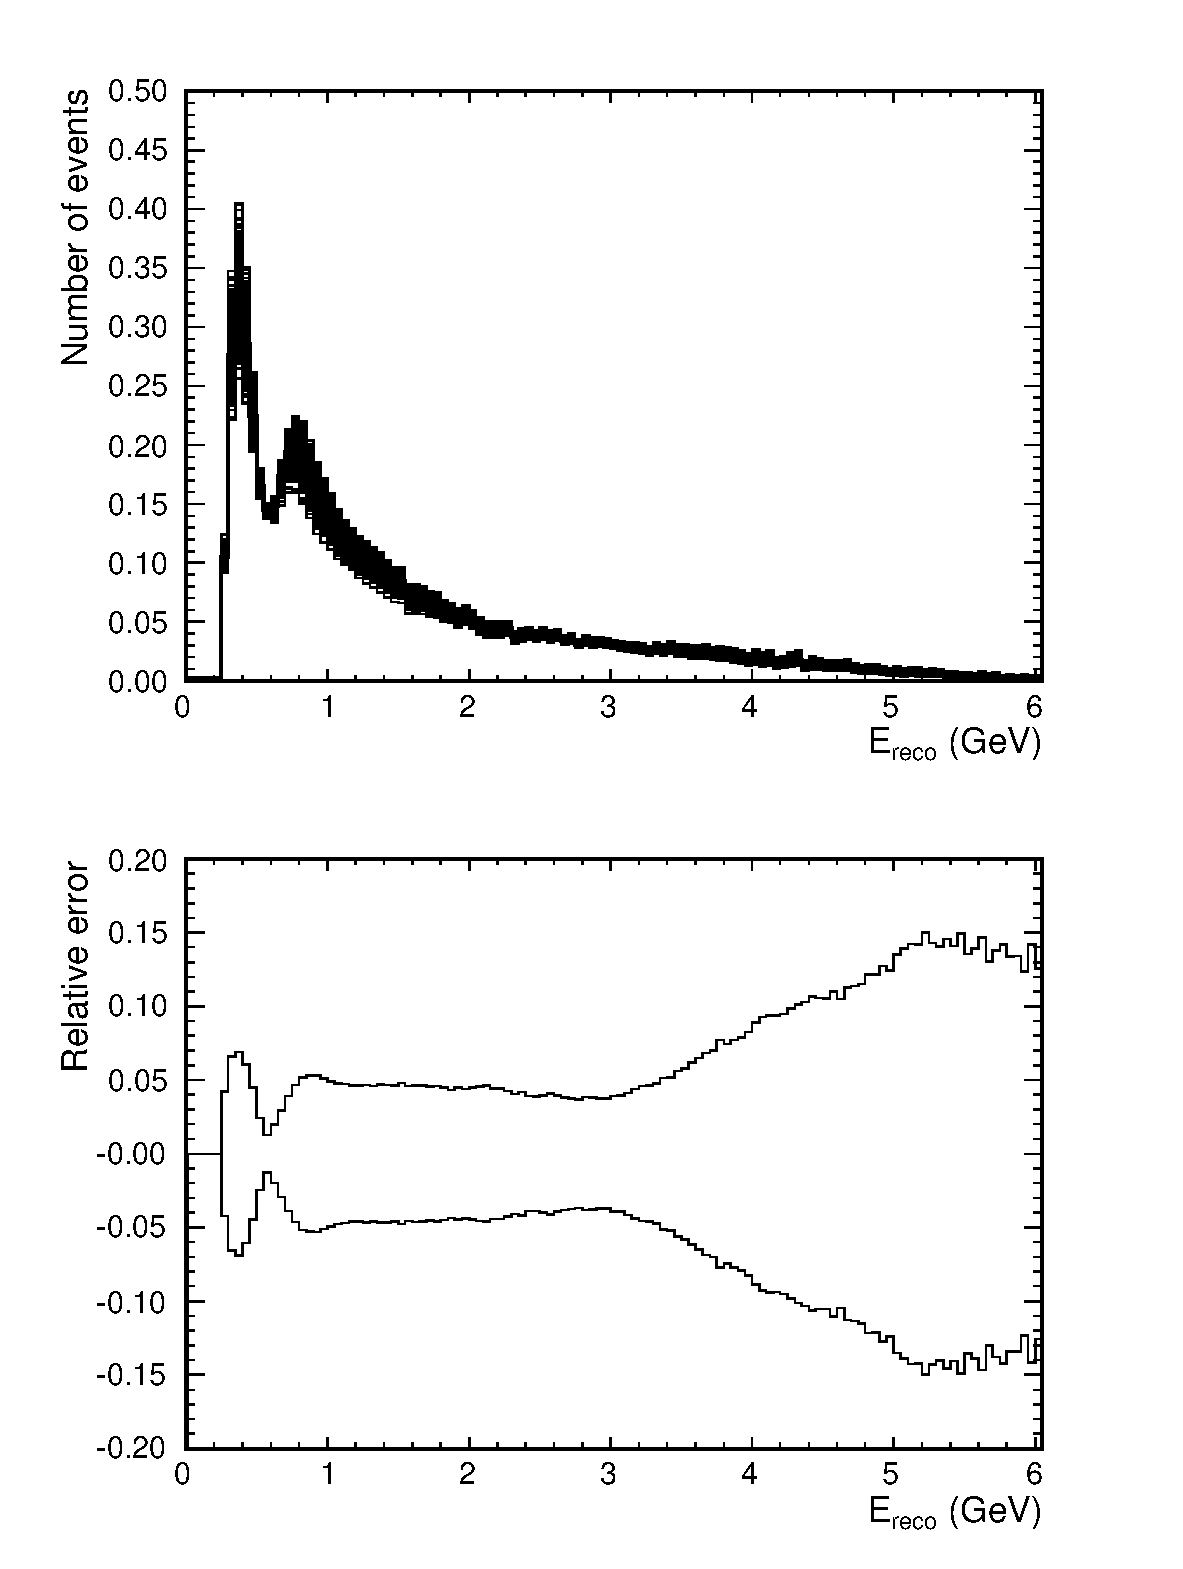
\includegraphics[width=19pc,height=19pc]{images/predicted_spectrum/systematic_variations/neut_sk_spectrum_twk_bshape_2p4Em3_1p0.eps}
\caption{
  Effect of beam shape variation to the NEUT
  reconstructed-energy spectrum of 1-ring muon-like events (after extrapolation).
  The plots were generated as described in Fig. \ref{fig:genie_sk_spectrum_twk_bshape_2p4Em3_1p0}.
}
\label{fig:neut_sk_spectrum_twk_bshape_2p4Em3_1p0}
\end{minipage}
\end{figure}


%
% CCQE
%

\begin{figure}[ht]
\begin{minipage}[t]{0.47\linewidth}
\centering
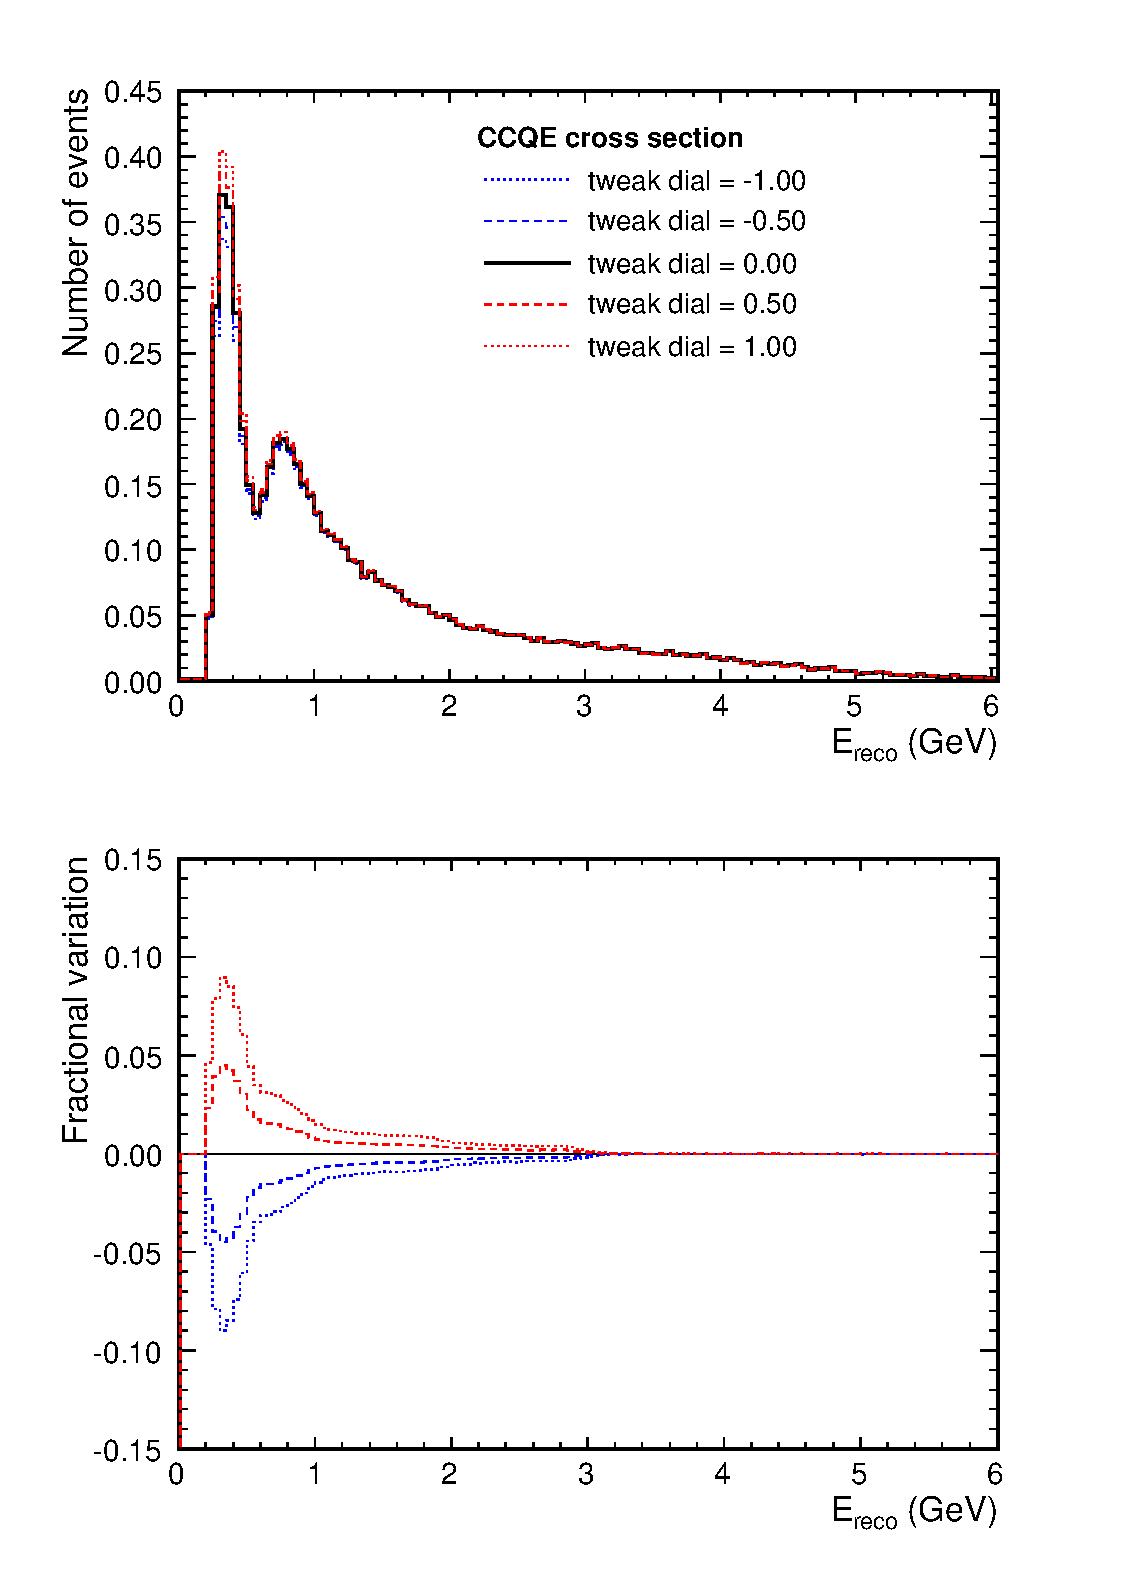
\includegraphics[width=19pc,height=21pc]{./images/predicted_spectrum/systematic_variations/genie_sk_spectrum_twk_ccqe_2p4Em3_1p0.eps}
\caption{
  Effect of CCQE cross section variation to the GENIE
  reconstructed-energy spectrum of 1-ring muon-like events (after extrapolation).
  All spectra have oscillations with $sin^{2}2\theta_{23}$ = 1.0 and $\Delta m^{2}_{23}$ = 2.4$\times10^{-3}$ $eV^{2}/c^{4}$ applied.  
}
\label{fig:genie_sk_spectrum_twk_ccqe_2p4Em3_1p0}
\end{minipage}
\hspace{0.06\linewidth}
\begin{minipage}[t]{0.47\linewidth}
\centering
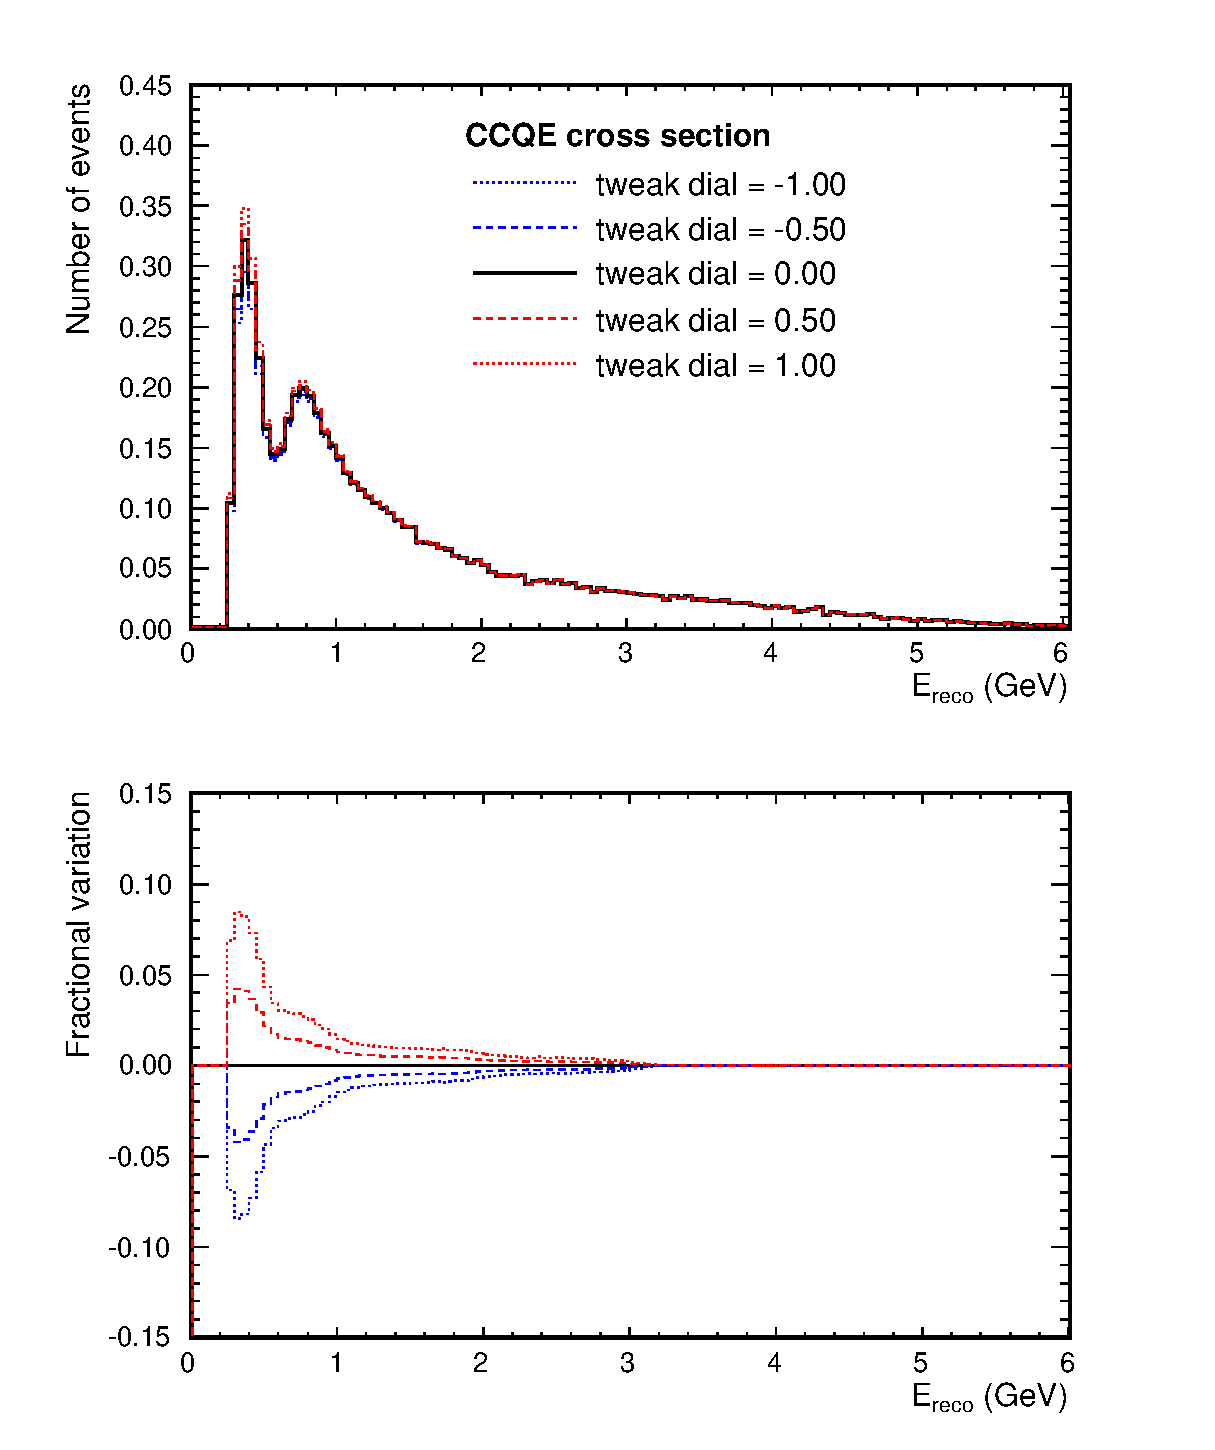
\includegraphics[width=19pc,height=21pc]{images/predicted_spectrum/systematic_variations/neut_sk_spectrum_twk_ccqe_2p4Em3_1p0.eps}
\caption{
  Effect of CCQE cross section variation to the NEUT
  reconstructed-energy spectrum of 1-ring muon-like events (after extrapolation).
  All spectra have oscillations with $sin^{2}2\theta_{23}$ = 1.0 and $\Delta m^{2}_{23}$ = 2.4$\times10^{-3}$ $eV^{2}/c^{4}$ applied.  
}
\label{fig:neut_sk_spectrum_twk_ccqe_2p4Em3_1p0}
\end{minipage}
\end{figure}

%
% CC1pi/CCQE
%

\begin{figure}[ht]
\begin{minipage}[t]{0.47\linewidth}
\centering
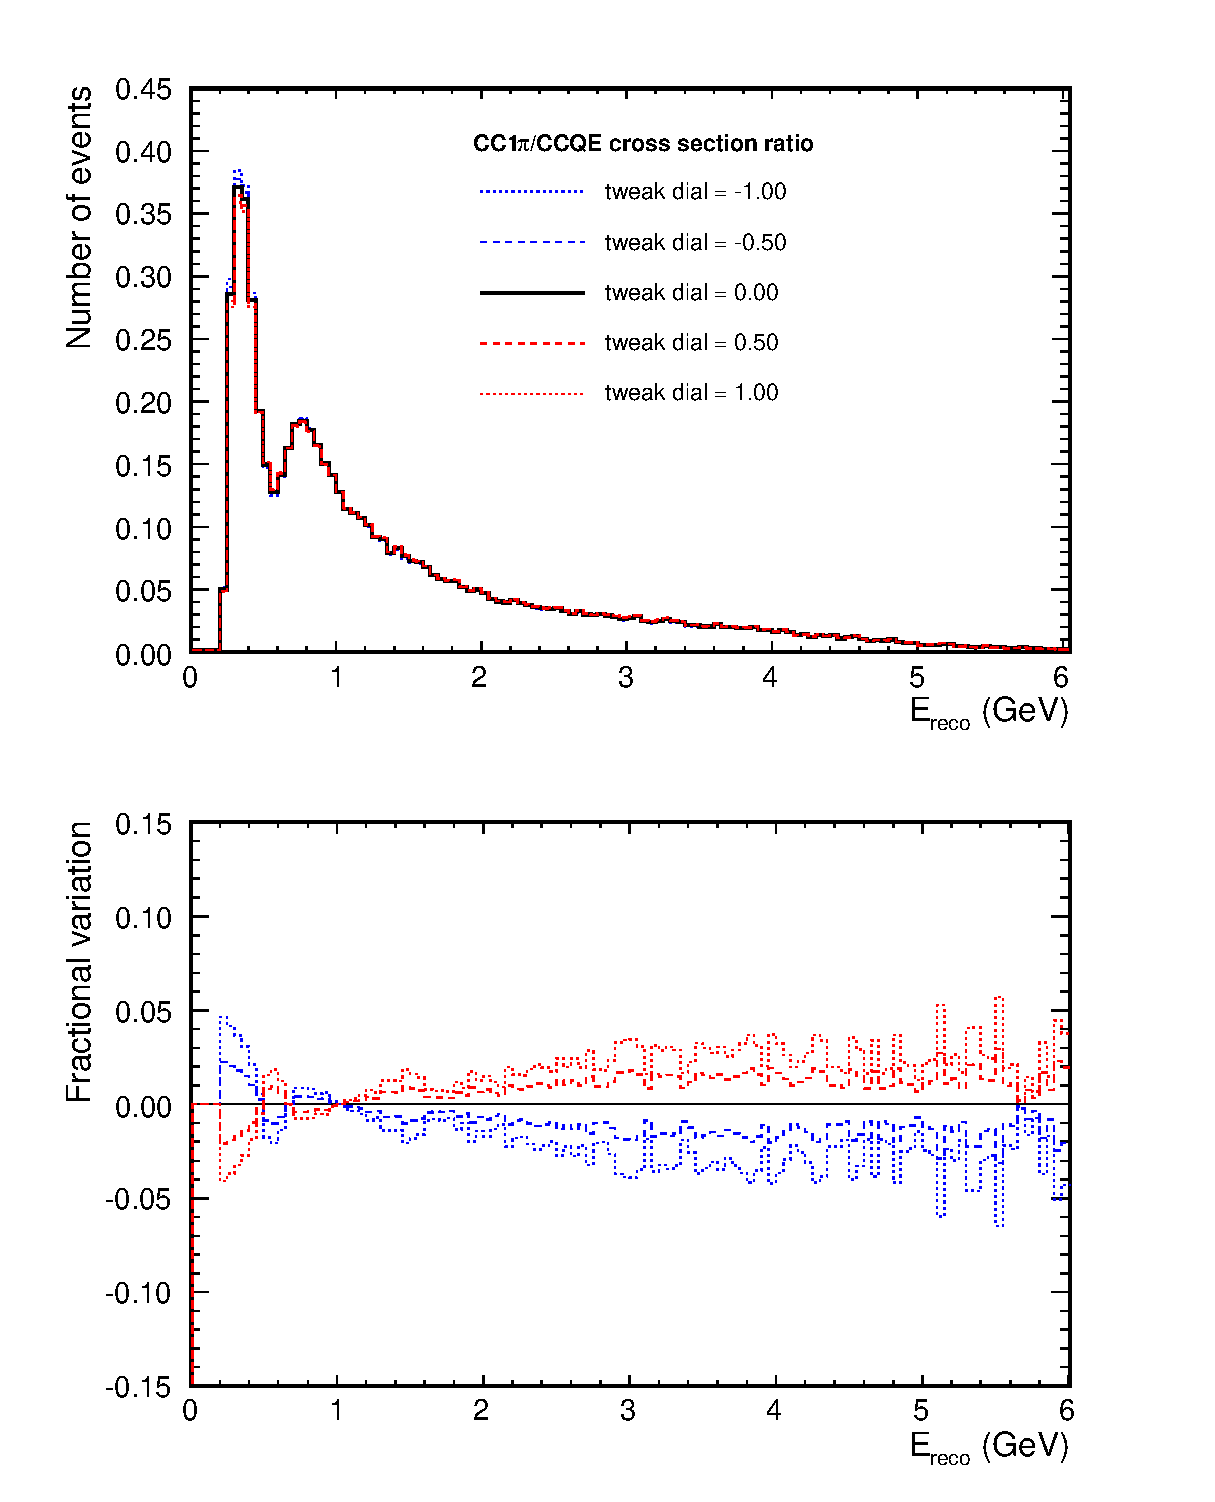
\includegraphics[width=19pc,height=21pc]{./images/predicted_spectrum/systematic_variations/genie_sk_spectrum_twk_cc1piccqe_2p4Em3_1p0.eps}
\caption{
  Effect of CC1$\pi$/CCQE cross section ratio variation to the GENIE
  reconstructed-energy spectrum of 1-ring muon-like events (after extrapolation).
  All spectra have oscillations with $sin^{2}2\theta_{23}$ = 1.0 and $\Delta m^{2}_{23}$ = 2.4$\times10^{-3}$ $eV^{2}/c^{4}$ applied.  
}
\label{fig:genie_sk_spectrum_twk_cc1piccqe_2p4Em3_1p0}
\end{minipage}
\hspace{0.06\linewidth}
\begin{minipage}[t]{0.47\linewidth}
\centering
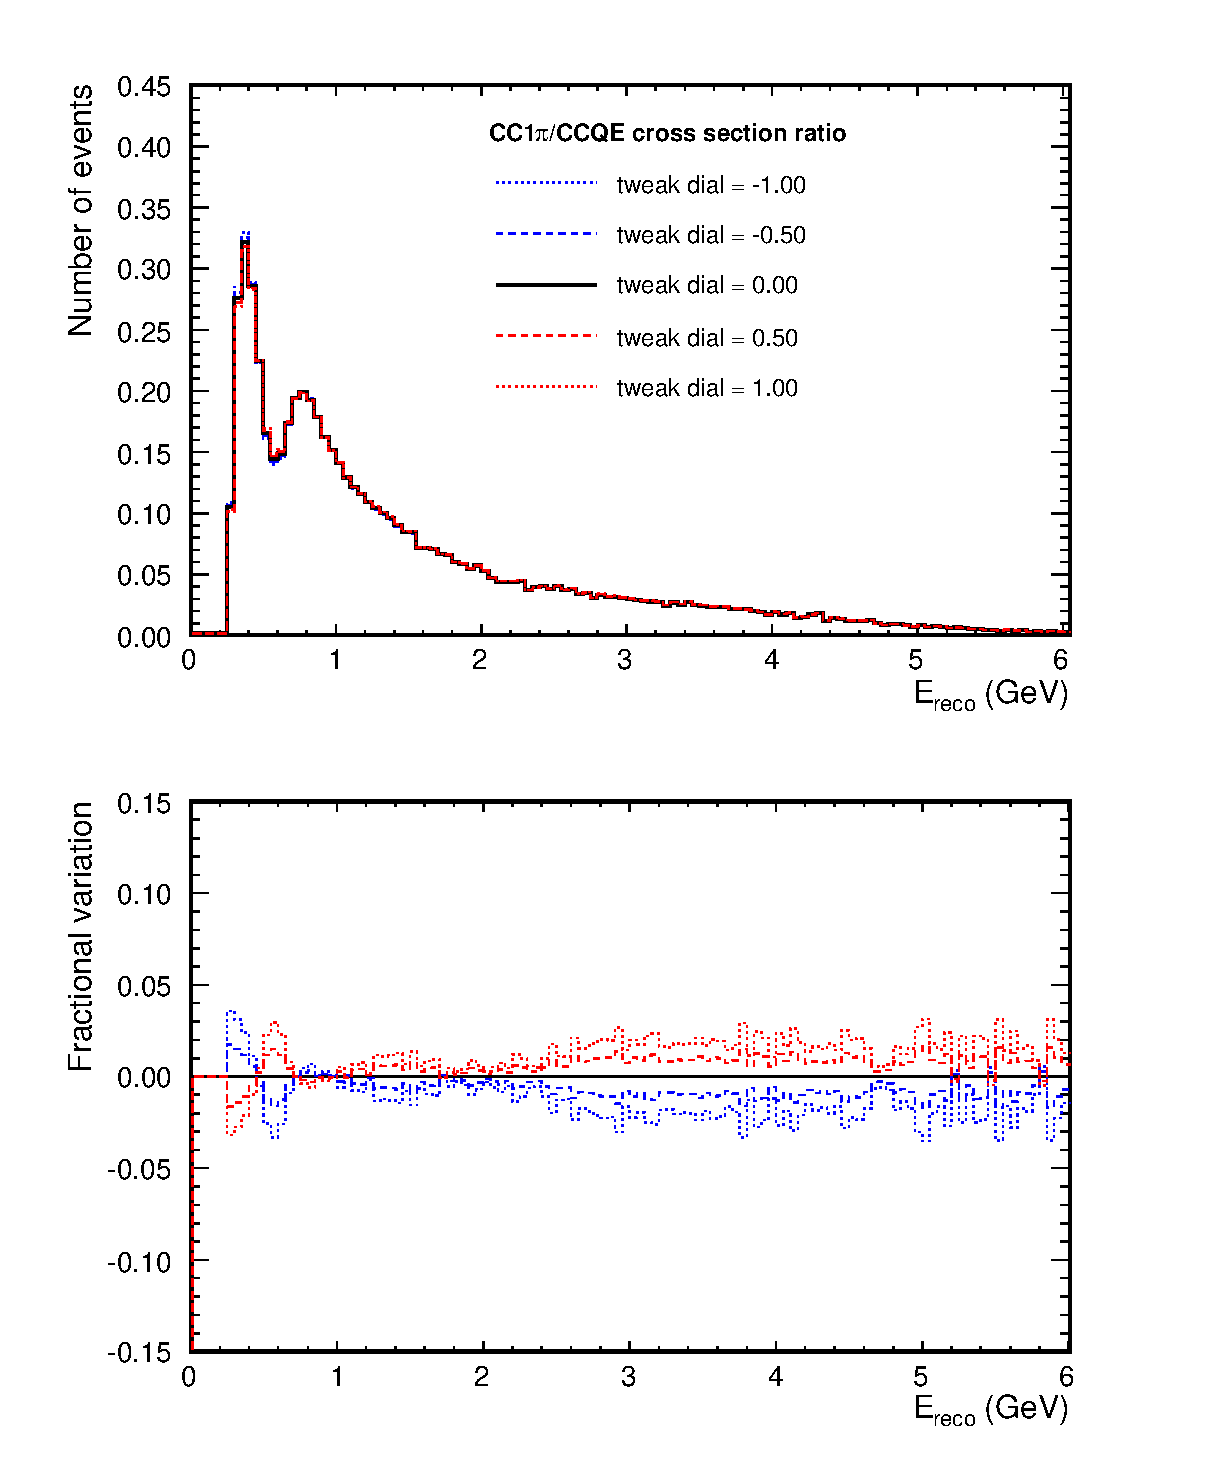
\includegraphics[width=19pc,height=21pc]{images/predicted_spectrum/systematic_variations/neut_sk_spectrum_twk_cc1piccqe_2p4Em3_1p0.eps}
\caption{
  Effect of CC1$\pi$/CCQE cross section ratio variation to the NEUT
  reconstructed-energy spectrum of 1-ring muon-like events (after extrapolation).
  All spectra have oscillations with $sin^{2}2\theta_{23}$ = 1.0 and $\Delta m^{2}_{23}$ = 2.4$\times10^{-3}$ $eV^{2}/c^{4}$ applied.  
}
\label{fig:neut_sk_spectrum_twk_cc1piccqe_2p4Em3_1p0}
\end{minipage}
\end{figure}


%
% CCoth/CCQE
%

\begin{figure}[ht]
\begin{minipage}[t]{0.47\linewidth}
\centering
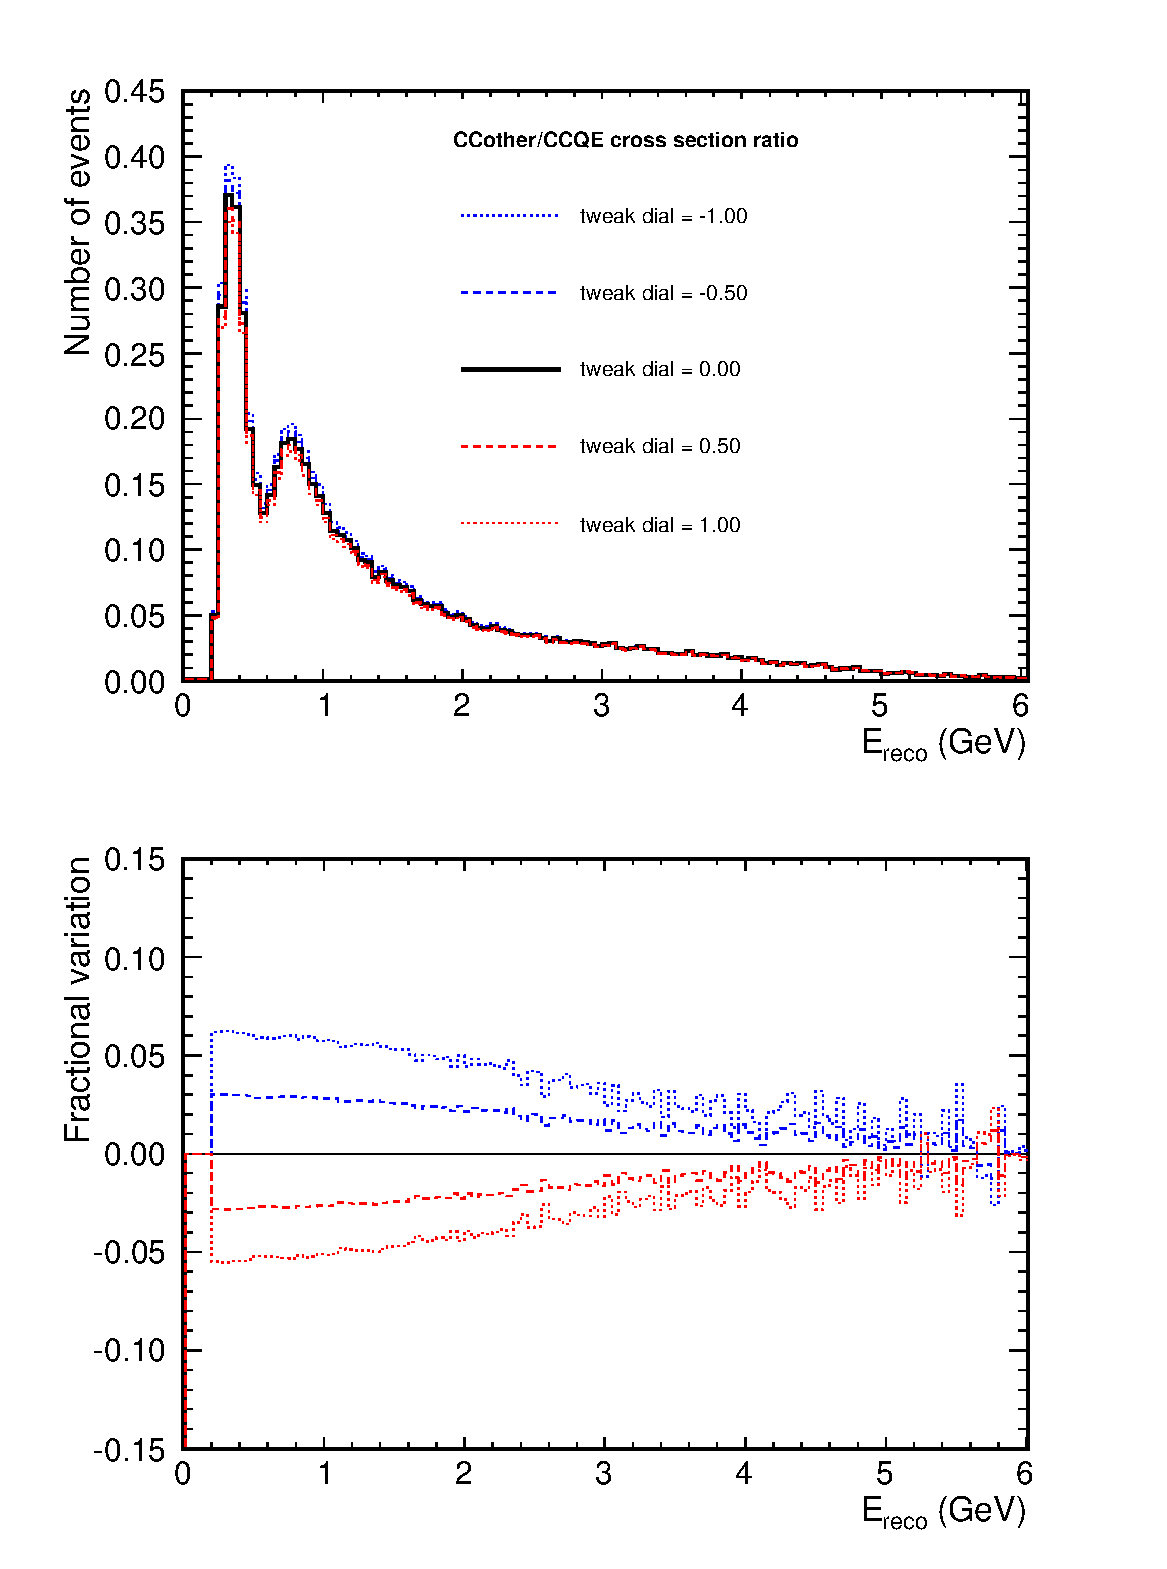
\includegraphics[width=19pc,height=21pc]{./images/predicted_spectrum/systematic_variations/genie_sk_spectrum_twk_ccothccqe_2p4Em3_1p0.eps}
\caption{
  Effect of CCother/CCQE cross section ratio variation to the GENIE
  reconstructed-energy spectrum of 1-ring muon-like events (after extrapolation).
  All spectra have oscillations with $sin^{2}2\theta_{23}$ = 1.0 and $\Delta m^{2}_{23}$ = 2.4$\times10^{-3}$ $eV^{2}/c^{4}$ applied.  
}
\label{fig:genie_sk_spectrum_twk_ccothccqe_2p4Em3_1p0}
\end{minipage}
\hspace{0.06\linewidth}
\begin{minipage}[t]{0.47\linewidth}
\centering
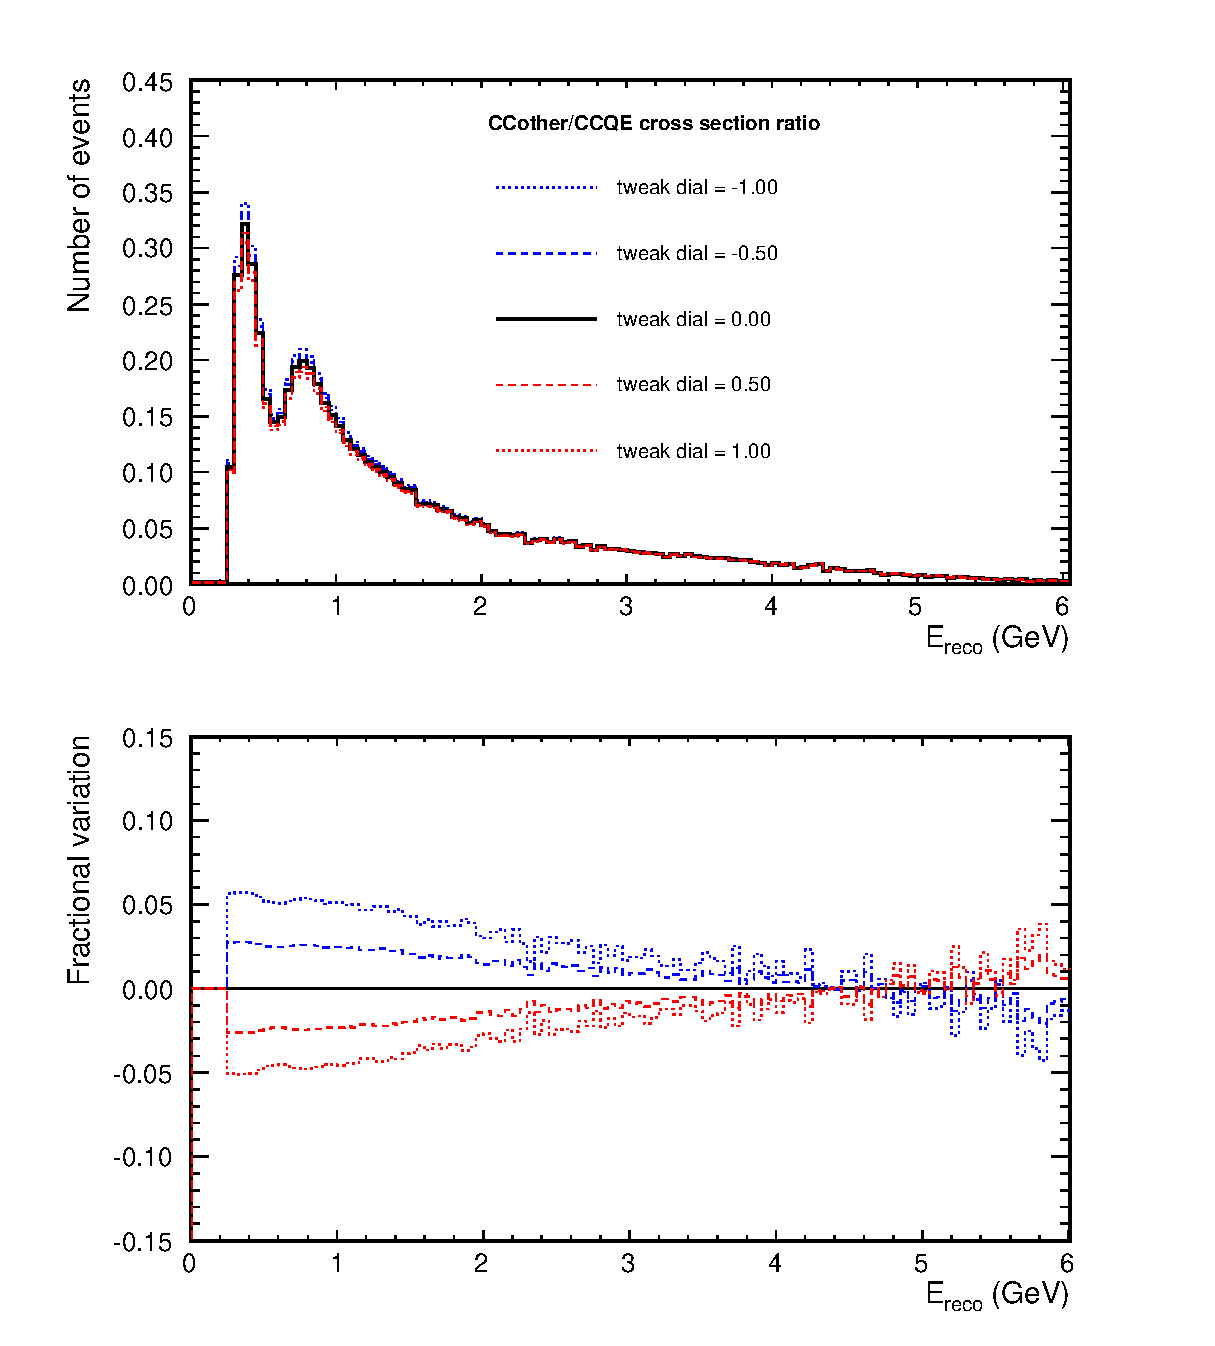
\includegraphics[width=19pc,height=21pc]{images/predicted_spectrum/systematic_variations/neut_sk_spectrum_twk_ccothccqe_2p4Em3_1p0.eps}
\caption{
  Effect of CCother/CCQE cross section ratio variation to the NEUT
  reconstructed-energy spectrum of 1-ring muon-like events (after extrapolation).
  All spectra have oscillations with $sin^{2}2\theta_{23}$ = 1.0 and $\Delta m^{2}_{23}$ = 2.4$\times10^{-3}$ $eV^{2}/c^{4}$ applied.  
}
\label{fig:neut_sk_spectrum_twk_ccothccqe_2p4Em3_1p0}
\end{minipage}
\end{figure}


%
% NC/CCQE
%

\begin{figure}[ht]
\begin{minipage}[t]{0.47\linewidth}
\centering
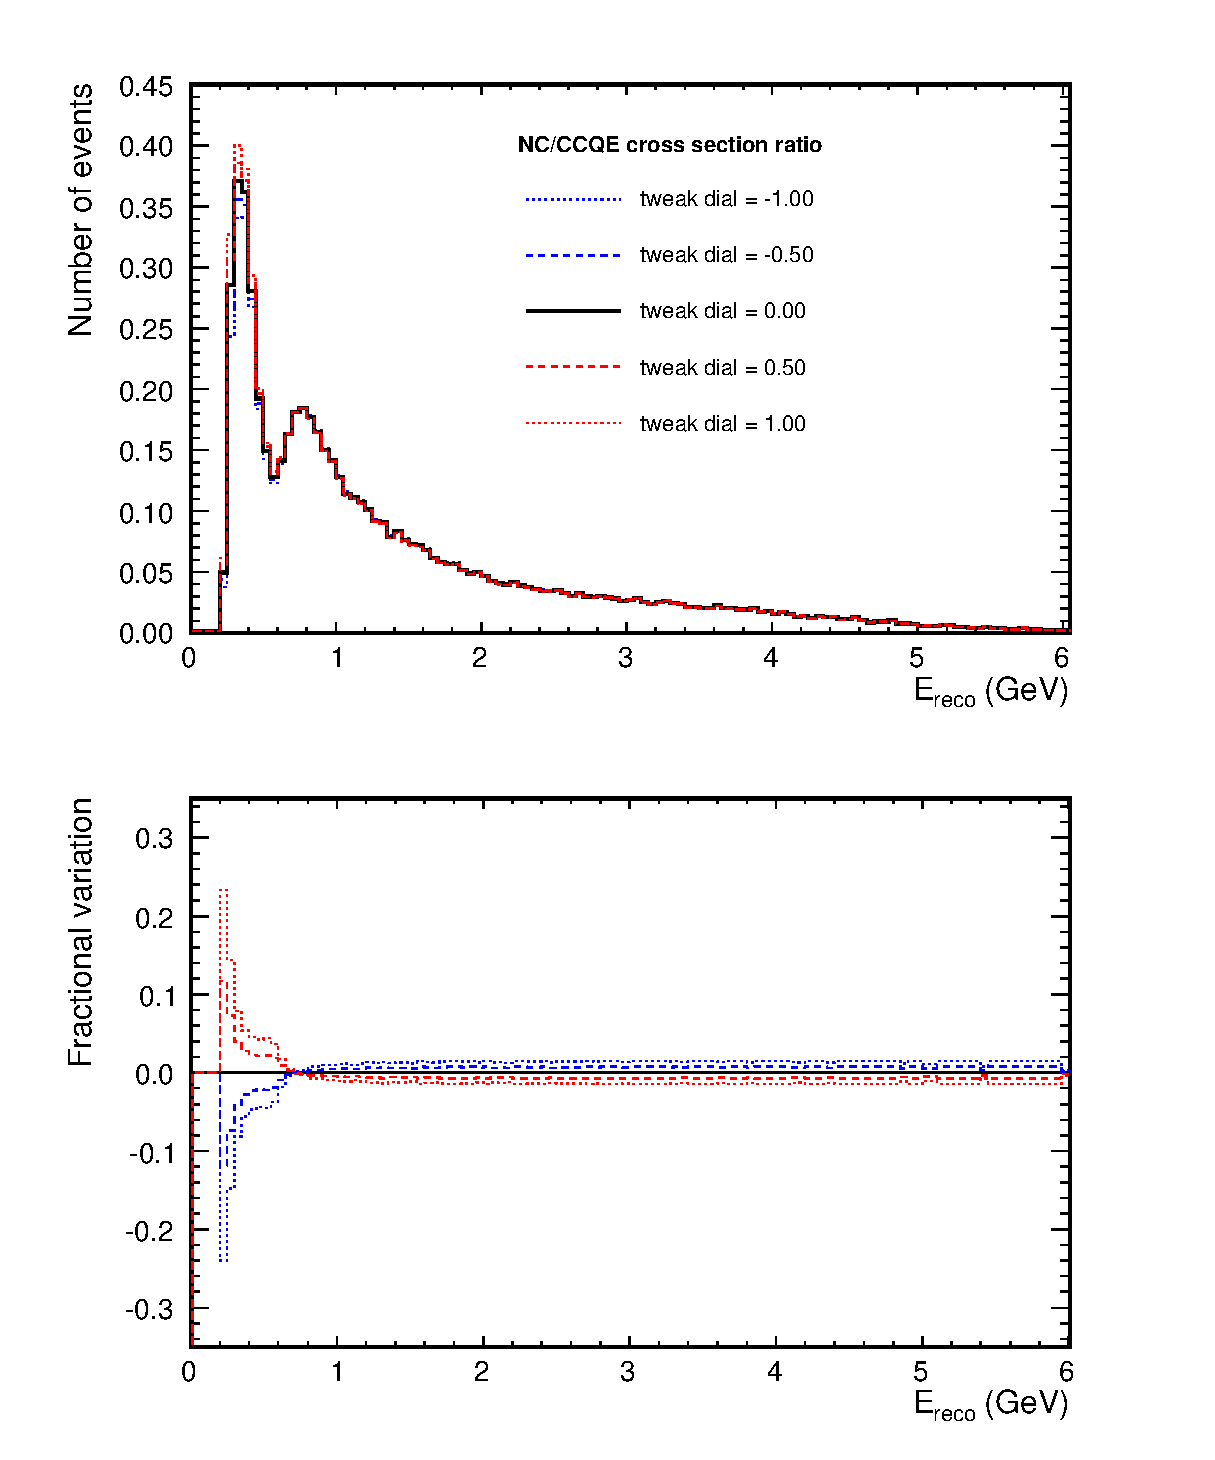
\includegraphics[width=19pc,height=21pc]{./images/predicted_spectrum/systematic_variations/genie_sk_spectrum_twk_ncccqe_2p4Em3_1p0.eps}
\caption{
  Effect of NC/CCQE cross section ratio variation to the GENIE
  reconstructed-energy spectrum of 1-ring muon-like events (after extrapolation).
  All spectra have oscillations with $sin^{2}2\theta_{23}$ = 1.0 and $\Delta m^{2}_{23}$ = 2.4$\times10^{-3}$ $eV^{2}/c^{4}$ applied.  
}
\label{fig:genie_sk_spectrum_twk_ncccqe_2p4Em3_1p0}
\end{minipage}
\hspace{0.06\linewidth}
\begin{minipage}[t]{0.47\linewidth}
\centering
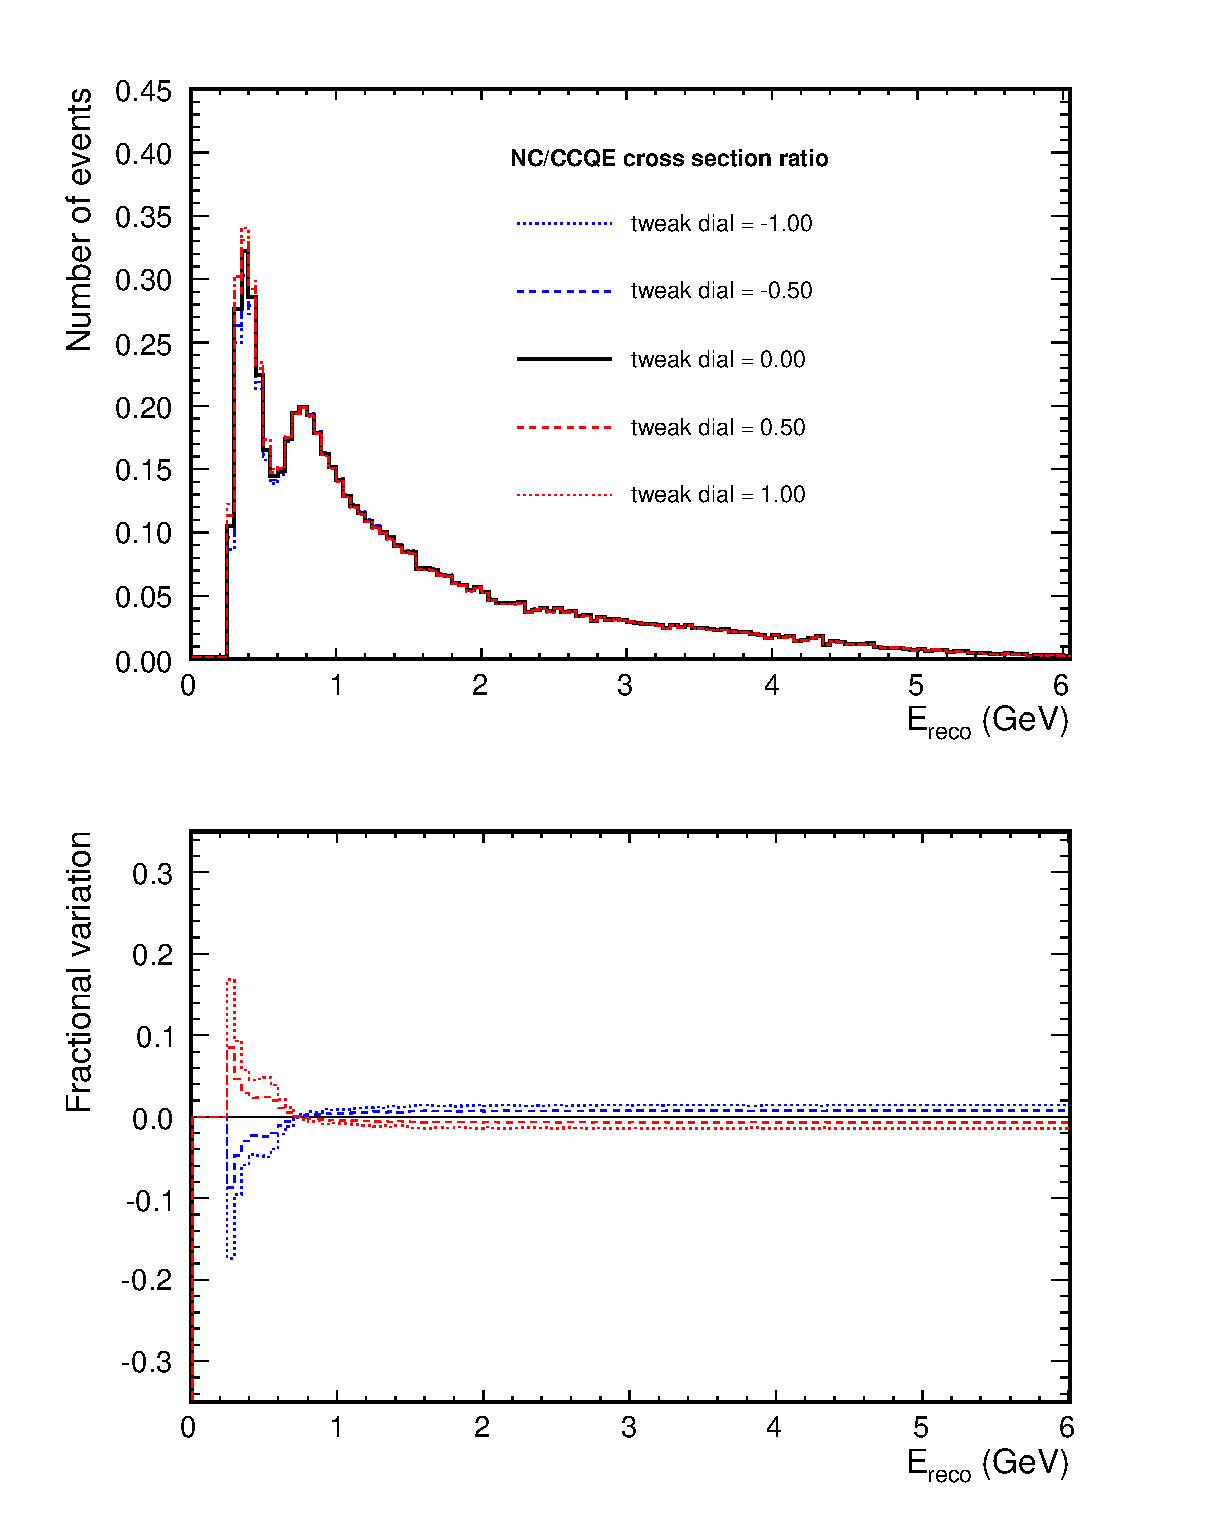
\includegraphics[width=19pc,height=21pc]{images/predicted_spectrum/systematic_variations/neut_sk_spectrum_twk_ncccqe_2p4Em3_1p0.eps}
\caption{
  Effect of NC/CCQE cross section ratio variation to the NEUT
  reconstructed-energy spectrum of 1-ring muon-like events (after extrapolation).
  All spectra have oscillations with $sin^{2}2\theta_{23}$ = 1.0 and $\Delta m^{2}_{23}$ = 2.4$\times10^{-3}$ $eV^{2}/c^{4}$ applied.  
}
\label{fig:neut_sk_spectrum_twk_ncccqe_2p4Em3_1p0}
\end{minipage}
\end{figure}


%
% NUCEFF
%

\begin{figure}[ht]
\begin{minipage}[t]{0.47\linewidth}
\centering
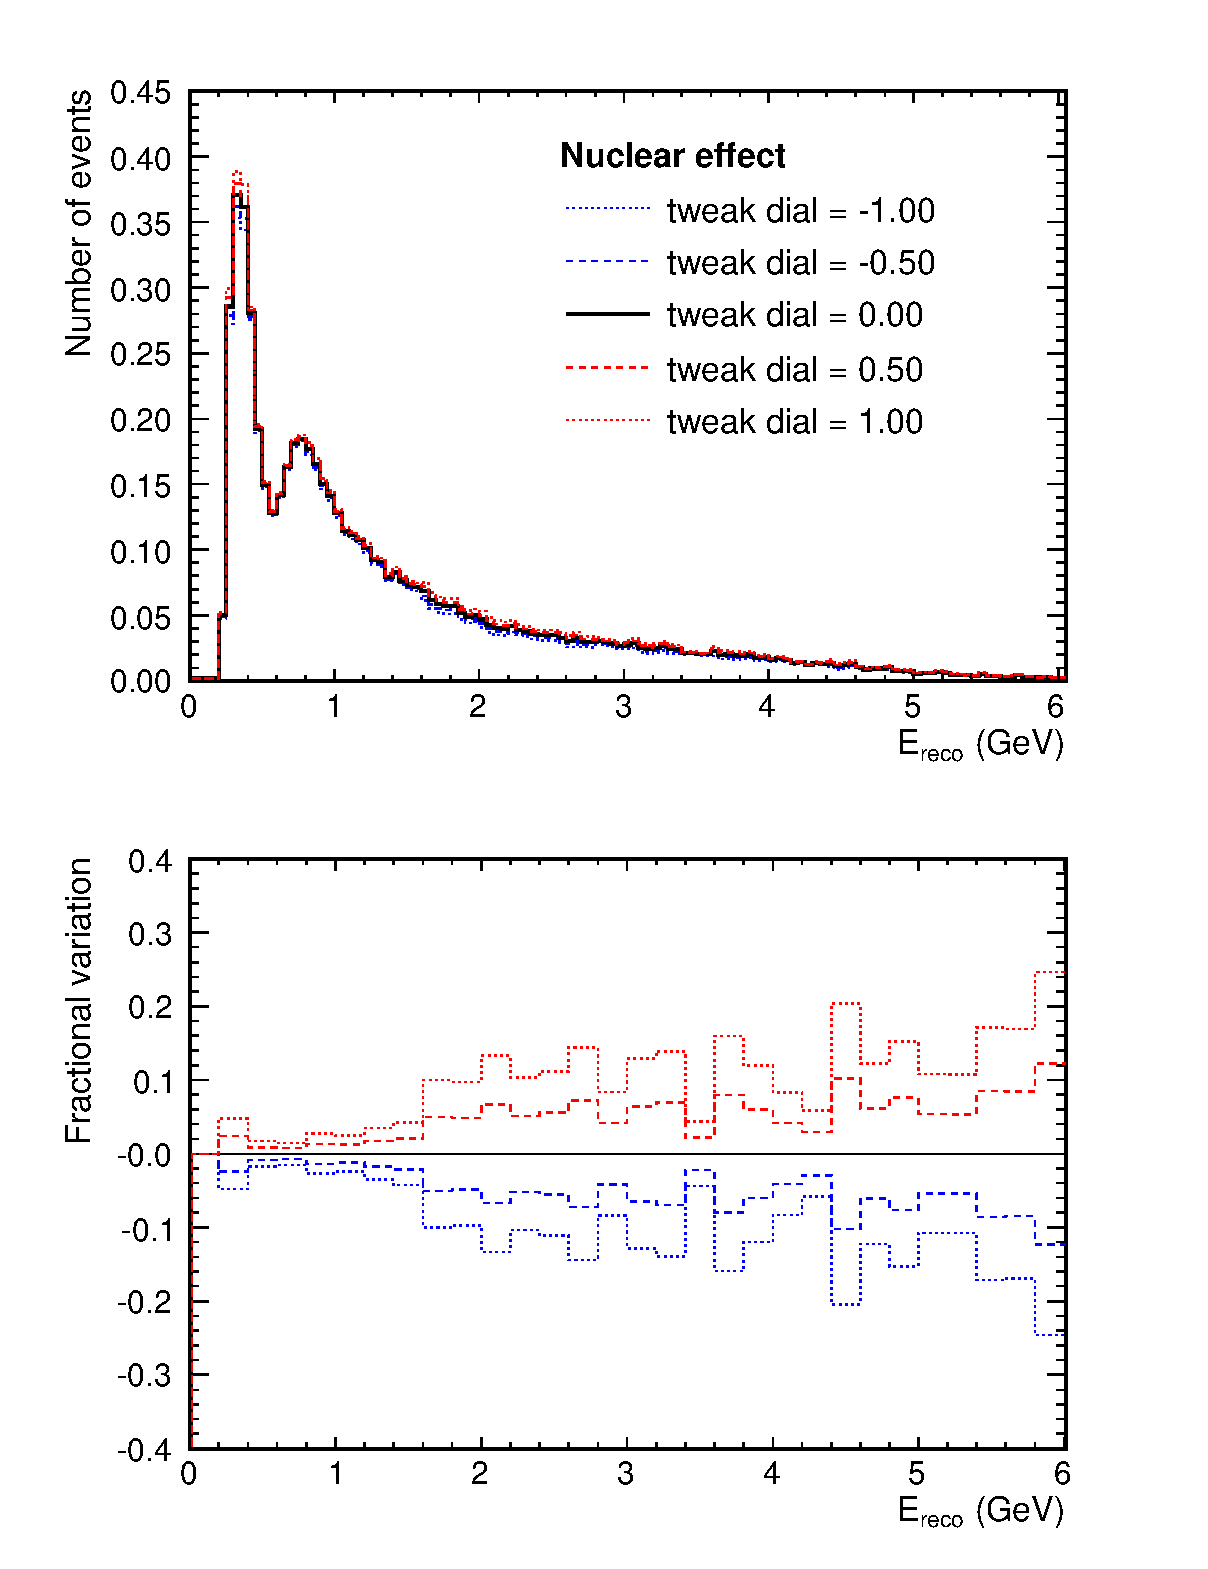
\includegraphics[width=19pc,height=21pc]{./images/predicted_spectrum/systematic_variations/genie_sk_spectrum_twk_nuceff_2p4Em3_1p0.eps}
\caption{
  Effect of FSI variation to the GENIE
  reconstructed-energy spectrum of 1-ring muon-like events (after extrapolation).
  All spectra have oscillations with $sin^{2}2\theta_{23}$ = 1.0 and $\Delta m^{2}_{23}$ = 2.4$\times10^{-3}$ $eV^{2}/c^{4}$ applied.  
}
\label{fig:genie_sk_spectrum_twk_nuceff_2p4Em3_1p0}
\end{minipage}
\hspace{0.06\linewidth}
\begin{minipage}[t]{0.47\linewidth}
\centering
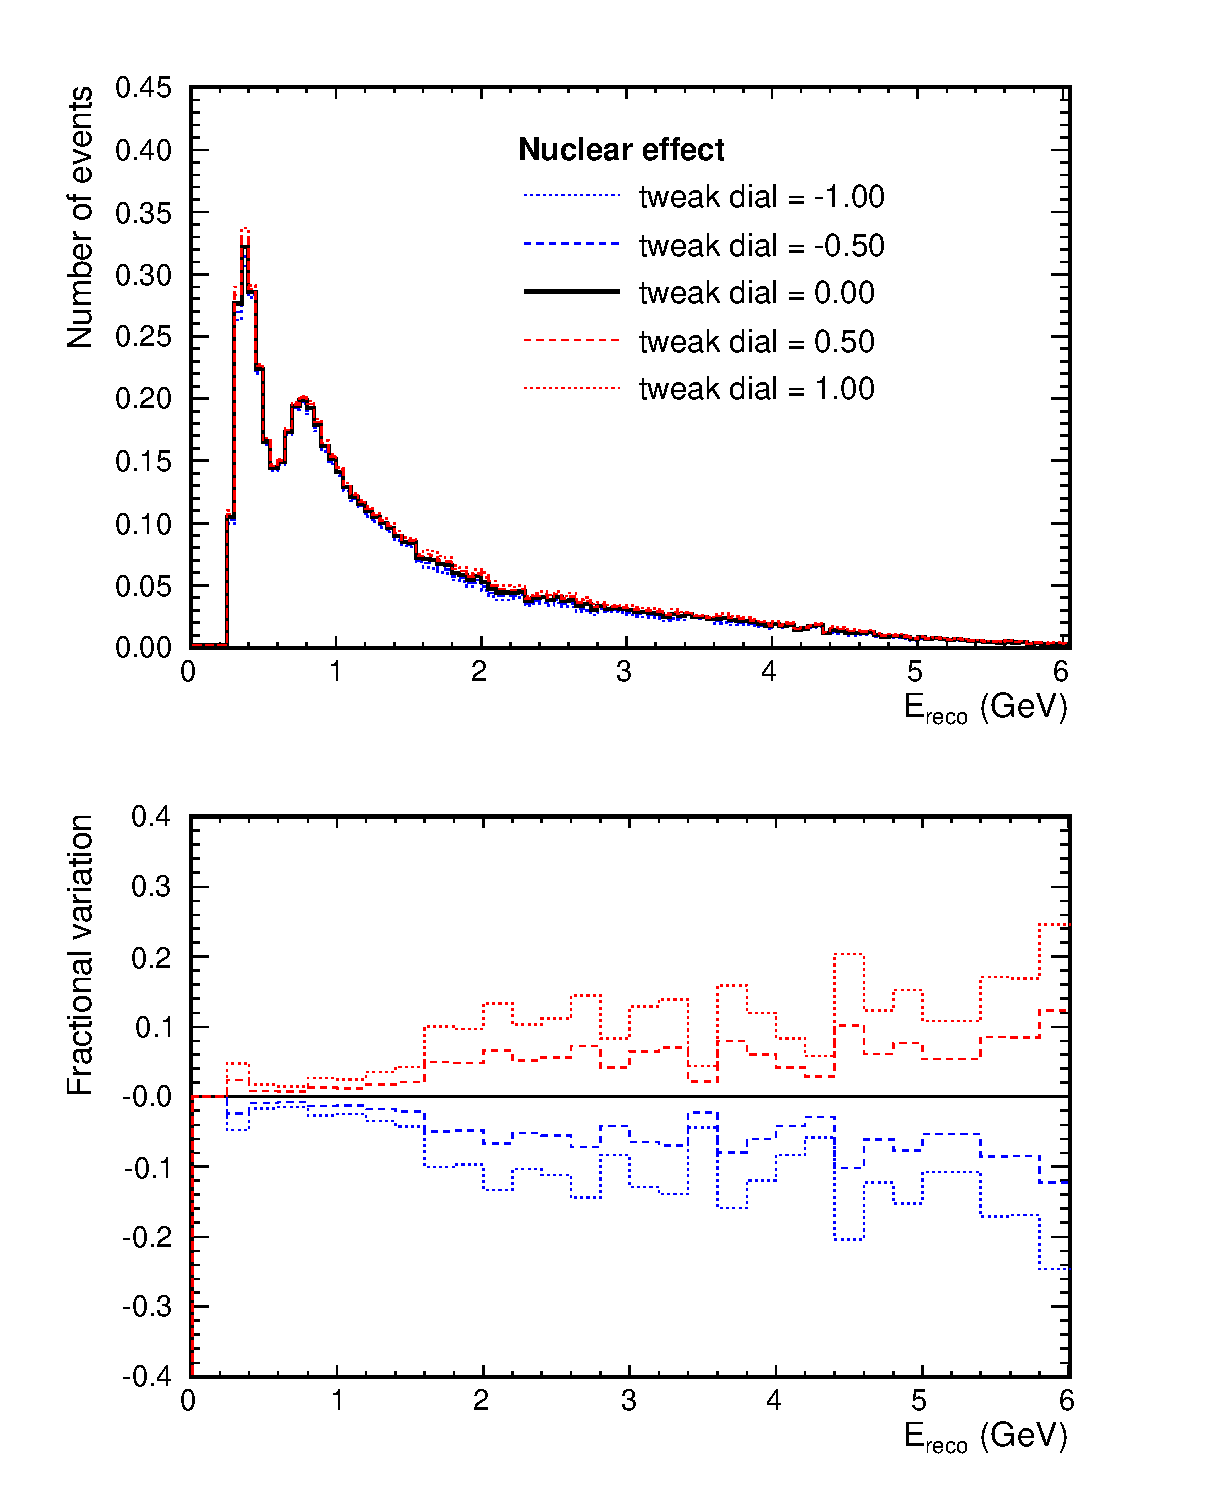
\includegraphics[width=19pc,height=21pc]{images/predicted_spectrum/systematic_variations/neut_sk_spectrum_twk_nuceff_2p4Em3_1p0.eps}
\caption{
  Effect of FSI variation to the NEUT
  reconstructed-energy spectrum of 1-ring muon-like events (after extrapolation).
  All spectra have oscillations with $sin^{2}2\theta_{23}$ = 1.0 and $\Delta m^{2}_{23}$ = 2.4$\times10^{-3}$ $eV^{2}/c^{4}$ applied.  
}
\label{fig:neut_sk_spectrum_twk_nuceff_2p4Em3_1p0}
\end{minipage}
\end{figure}

\clearpage

%
% ------------------------------------------------------------------------------------------
% GENIE TABLES
% ------------------------------------------------------------------------------------------
%

%
%
% SK CCQE efficiency: GENIE
%
%

\begin{table}
\centering
\begin{tabular}{| l | r | r  r | r  r |}
\hline
{\bf Component} &  {\bf Nominal}   &  \multicolumn {2}{c|} { {\bf +1$\sigma$} } &  \multicolumn {2}{c|} { {\bf -1$\sigma$} } \\
\hline
                                          $N_{SK}$ (1 $\mu$-like ring) &          6.2043 &          6.5019 &  4.80 \%  &          5.9066 & -4.80 \%  \\ 
\hline
                                             SK MC (1 $\mu$-like ring) &          5.3721 &          5.6299 &  4.80 \%  &          5.1144 & -4.80 \%  \\ 
\hline
                           SK MC (1 $\mu$-like ring): $\nu_{\mu}$ CCQE &          3.0985 &          3.3402 &  7.80 \%  &          2.8568 & -7.80 \%  \\ 
                       SK MC (1 $\mu$-like ring): $\nu_{\mu}$ CC1$\pi$ &          1.2545 &          1.2545 &  0.00 \%  &          1.2545 &  0.00 \%  \\ 
                       SK MC (1 $\mu$-like ring): $\nu_{\mu}$ CC other &          0.2177 &          0.2177 &  0.00 \%  &          0.2177 &  0.00 \%  \\ 
                         SK MC (1 $\mu$-like ring): $\nu_{\mu}$ CC all &          4.5707 &          4.8124 &  5.29 \%  &          4.3290 & -5.29 \%  \\ 
                         SK MC (1 $\mu$-like ring): $\nu_{\mu}$ NC all &          0.4087 &          0.4087 &  0.00 \%  &          0.4087 &  0.00 \%  \\ 
                     SK MC (1 $\mu$-like ring): $\bar{\nu_{\mu}}$ CCQE &          0.2056 &          0.2217 &  7.80 \%  &          0.1896 & -7.80 \%  \\ 
                 SK MC (1 $\mu$-like ring): $\bar{\nu_{\mu}}$ CC1$\pi$ &          0.1271 &          0.1271 &  0.00 \%  &          0.1271 &  0.00 \%  \\ 
                 SK MC (1 $\mu$-like ring): $\bar{\nu_{\mu}}$ CC other &          0.0215 &          0.0215 &  0.00 \%  &          0.0215 &  0.00 \%  \\ 
                   SK MC (1 $\mu$-like ring): $\bar{\nu_{\mu}}$ CC all &          0.3542 &          0.3702 &  4.53 \%  &          0.3382 & -4.53 \%  \\ 
                   SK MC (1 $\mu$-like ring): $\bar{\nu_{\mu}}$ NC all &          0.0236 &          0.0236 &  0.00 \%  &          0.0236 &  0.00 \%  \\ 
                             SK MC (1 $\mu$-like ring): $\nu_{e}$ CCQE &          0.0014 &          0.0014 &  0.00 \%  &          0.0014 &  0.00 \%  \\ 
                         SK MC (1 $\mu$-like ring): $\nu_{e}$ CC1$\pi$ &          0.0008 &          0.0008 &  0.00 \%  &          0.0008 &  0.00 \%  \\ 
                         SK MC (1 $\mu$-like ring): $\nu_{e}$ CC other &          0.0002 &          0.0002 &  0.00 \%  &          0.0002 &  0.00 \%  \\ 
                           SK MC (1 $\mu$-like ring): $\nu_{e}$ CC all &          0.0024 &          0.0024 &  0.00 \%  &          0.0024 &  0.00 \%  \\ 
                           SK MC (1 $\mu$-like ring): $\nu_{e}$ NC all &          0.0125 &          0.0125 &  0.00 \%  &          0.0125 &  0.00 \%  \\ 
\hline
                                       ND280 CC-like Observed/MC ratio &          1.1549 &          1.1549 &  0.00 \%  &          1.1549 &  0.00 \%  \\ 
                                                ND280 Observed CC-like &       1445.0000 &       1445.0000 &  0.00 \%  &       1445.0000 &  0.00 \%  \\ 
                                               ND280 MC: Total CC-like &       1251.1924 &       1251.1924 &  0.00 \%  &       1251.1924 &  0.00 \%  \\ 
                                                    ND280 MC: Total CC &       1199.6960 &       1199.6960 &  0.00 \%  &       1199.6960 &  0.00 \%  \\ 
                                         ND280 MC: Total NC background &         51.4964 &         51.4964 &  0.00 \%  &         51.4964 &  0.00 \%  \\ 
\hline
                                            ND280 MC: $\nu_{\mu}$ CCQE &        617.6298 &        617.6298 &  0.00 \%  &        617.6298 &  0.00 \%  \\ 
                                        ND280 MC: $\nu_{\mu}$ CC1$\pi$ &        291.9388 &        291.9388 &  0.00 \%  &        291.9388 &  0.00 \%  \\ 
                                        ND280 MC: $\nu_{\mu}$ CC other &        280.0197 &        280.0197 &  0.00 \%  &        280.0197 &  0.00 \%  \\ 
                                          ND280 MC: $\nu_{\mu}$ CC all &       1189.5883 &       1189.5883 &  0.00 \%  &       1189.5883 &  0.00 \%  \\ 
                                          ND280 MC: $\nu_{\mu}$ NC all &         48.8820 &         48.8820 &  0.00 \%  &         48.8820 &  0.00 \%  \\ 
                                      ND280 MC: $\bar{\nu_{\mu}}$ CCQE &          0.3815 &          0.3815 &  0.00 \%  &          0.3815 &  0.00 \%  \\ 
                                  ND280 MC: $\bar{\nu_{\mu}}$ CC1$\pi$ &          3.0898 &          3.0898 &  0.00 \%  &          3.0898 &  0.00 \%  \\ 
                                  ND280 MC: $\bar{\nu_{\mu}}$ CC other &          4.9767 &          4.9767 &  0.00 \%  &          4.9767 &  0.00 \%  \\ 
                                    ND280 MC: $\bar{\nu_{\mu}}$ CC all &          8.4480 &          8.4480 &  0.00 \%  &          8.4480 &  0.00 \%  \\ 
                                    ND280 MC: $\bar{\nu_{\mu}}$ NC all &          1.8276 &          1.8276 &  0.00 \%  &          1.8276 &  0.00 \%  \\ 
                                              ND280 MC: $\nu_{e}$ CCQE &          0.1889 &          0.1889 &  0.00 \%  &          0.1889 &  0.00 \%  \\ 
                                          ND280 MC: $\nu_{e}$ CC1$\pi$ &          0.4312 &          0.4312 &  0.00 \%  &          0.4312 &  0.00 \%  \\ 
                                          ND280 MC: $\nu_{e}$ CC other &          1.0397 &          1.0397 &  0.00 \%  &          1.0397 &  0.00 \%  \\ 
                                            ND280 MC: $\nu_{e}$ CC all &          1.6598 &          1.6598 &  0.00 \%  &          1.6598 &  0.00 \%  \\ 
                                            ND280 MC: $\nu_{e}$ NC all &          0.7868 &          0.7868 &  0.00 \%  &          0.7868 &  0.00 \%  \\ 
\hline
\end{tabular}
\caption{ 
  Effect of SuperK CCQE efficiency variation
  on various components of the oscillation analysis (GENIE).
  Oscillations with parameters $sin^{2}2\theta_{23}$ = 1.0 and $\Delta m^{2}_{23}$ = 2.4$\times10^{-3}$ $eV^{2}/c^{4}$ were applied.  
}
\label{tab:genie_sk_ccqe_eff}
\end{table}

%
%
% SK CCnonQE efficiency: GENIE
%
%

\begin{table}
\centering
\begin{tabular}{| l | r | r  r | r  r |}
\hline
{\bf Component} &  {\bf Nominal}   &  \multicolumn {2}{c|} { {\bf +1$\sigma$} } &  \multicolumn {2}{c|} { {\bf -1$\sigma$} } \\
\hline
                                          $N_{SK}$ (1 $\mu$-like ring) &          6.2043 &          6.6816 &  7.69 \%  &          5.7270 & -7.69 \%  \\ 
\hline
                                             SK MC (1 $\mu$-like ring) &          5.3721 &          5.7854 &  7.69 \%  &          4.9588 & -7.69 \%  \\ 
\hline
                           SK MC (1 $\mu$-like ring): $\nu_{\mu}$ CCQE &          3.0985 &          3.0985 &  0.00 \%  &          3.0985 &  0.00 \%  \\ 
                       SK MC (1 $\mu$-like ring): $\nu_{\mu}$ CC1$\pi$ &          1.2545 &          1.5744 & 25.50 \%  &          0.9346 & -25.50 \%  \\ 
                       SK MC (1 $\mu$-like ring): $\nu_{\mu}$ CC other &          0.2177 &          0.2732 & 25.50 \%  &          0.1622 & -25.50 \%  \\ 
                         SK MC (1 $\mu$-like ring): $\nu_{\mu}$ CC all &          4.5707 &          4.9461 &  8.21 \%  &          4.1953 & -8.21 \%  \\ 
                         SK MC (1 $\mu$-like ring): $\nu_{\mu}$ NC all &          0.4087 &          0.4087 &  0.00 \%  &          0.4087 &  0.00 \%  \\ 
                     SK MC (1 $\mu$-like ring): $\bar{\nu_{\mu}}$ CCQE &          0.2056 &          0.2056 &  0.00 \%  &          0.2056 &  0.00 \%  \\ 
                 SK MC (1 $\mu$-like ring): $\bar{\nu_{\mu}}$ CC1$\pi$ &          0.1271 &          0.1595 & 25.50 \%  &          0.0947 & -25.50 \%  \\ 
                 SK MC (1 $\mu$-like ring): $\bar{\nu_{\mu}}$ CC other &          0.0215 &          0.0270 & 25.50 \%  &          0.0160 & -25.50 \%  \\ 
                   SK MC (1 $\mu$-like ring): $\bar{\nu_{\mu}}$ CC all &          0.3542 &          0.3921 & 10.69 \%  &          0.3163 & -10.69 \%  \\ 
                   SK MC (1 $\mu$-like ring): $\bar{\nu_{\mu}}$ NC all &          0.0236 &          0.0236 &  0.00 \%  &          0.0236 &  0.00 \%  \\ 
                             SK MC (1 $\mu$-like ring): $\nu_{e}$ CCQE &          0.0014 &          0.0014 &  0.00 \%  &          0.0014 &  0.00 \%  \\ 
                         SK MC (1 $\mu$-like ring): $\nu_{e}$ CC1$\pi$ &          0.0008 &          0.0008 &  0.00 \%  &          0.0008 &  0.00 \%  \\ 
                         SK MC (1 $\mu$-like ring): $\nu_{e}$ CC other &          0.0002 &          0.0002 &  0.00 \%  &          0.0002 &  0.00 \%  \\ 
                           SK MC (1 $\mu$-like ring): $\nu_{e}$ CC all &          0.0024 &          0.0024 &  0.00 \%  &          0.0024 &  0.00 \%  \\ 
                           SK MC (1 $\mu$-like ring): $\nu_{e}$ NC all &          0.0125 &          0.0125 &  0.00 \%  &          0.0125 &  0.00 \%  \\ 
\hline
                                       ND280 CC-like Observed/MC ratio &          1.1549 &          1.1549 &  0.00 \%  &          1.1549 &  0.00 \%  \\ 
                                                ND280 Observed CC-like &       1445.0000 &       1445.0000 &  0.00 \%  &       1445.0000 &  0.00 \%  \\ 
                                               ND280 MC: Total CC-like &       1251.1924 &       1251.1924 &  0.00 \%  &       1251.1924 &  0.00 \%  \\ 
                                                    ND280 MC: Total CC &       1199.6960 &       1199.6960 &  0.00 \%  &       1199.6960 &  0.00 \%  \\ 
                                         ND280 MC: Total NC background &         51.4964 &         51.4964 &  0.00 \%  &         51.4964 &  0.00 \%  \\ 
\hline
                                            ND280 MC: $\nu_{\mu}$ CCQE &        617.6298 &        617.6298 &  0.00 \%  &        617.6298 &  0.00 \%  \\ 
                                        ND280 MC: $\nu_{\mu}$ CC1$\pi$ &        291.9388 &        291.9388 &  0.00 \%  &        291.9388 &  0.00 \%  \\ 
                                        ND280 MC: $\nu_{\mu}$ CC other &        280.0197 &        280.0197 &  0.00 \%  &        280.0197 &  0.00 \%  \\ 
                                          ND280 MC: $\nu_{\mu}$ CC all &       1189.5883 &       1189.5883 &  0.00 \%  &       1189.5883 &  0.00 \%  \\ 
                                          ND280 MC: $\nu_{\mu}$ NC all &         48.8820 &         48.8820 &  0.00 \%  &         48.8820 &  0.00 \%  \\ 
                                      ND280 MC: $\bar{\nu_{\mu}}$ CCQE &          0.3815 &          0.3815 &  0.00 \%  &          0.3815 &  0.00 \%  \\ 
                                  ND280 MC: $\bar{\nu_{\mu}}$ CC1$\pi$ &          3.0898 &          3.0898 &  0.00 \%  &          3.0898 &  0.00 \%  \\ 
                                  ND280 MC: $\bar{\nu_{\mu}}$ CC other &          4.9767 &          4.9767 &  0.00 \%  &          4.9767 &  0.00 \%  \\ 
                                    ND280 MC: $\bar{\nu_{\mu}}$ CC all &          8.4480 &          8.4480 &  0.00 \%  &          8.4480 &  0.00 \%  \\ 
                                    ND280 MC: $\bar{\nu_{\mu}}$ NC all &          1.8276 &          1.8276 &  0.00 \%  &          1.8276 &  0.00 \%  \\ 
                                              ND280 MC: $\nu_{e}$ CCQE &          0.1889 &          0.1889 &  0.00 \%  &          0.1889 &  0.00 \%  \\ 
                                          ND280 MC: $\nu_{e}$ CC1$\pi$ &          0.4312 &          0.4312 &  0.00 \%  &          0.4312 &  0.00 \%  \\ 
                                          ND280 MC: $\nu_{e}$ CC other &          1.0397 &          1.0397 &  0.00 \%  &          1.0397 &  0.00 \%  \\ 
                                            ND280 MC: $\nu_{e}$ CC all &          1.6598 &          1.6598 &  0.00 \%  &          1.6598 &  0.00 \%  \\ 
                                            ND280 MC: $\nu_{e}$ NC all &          0.7868 &          0.7868 &  0.00 \%  &          0.7868 &  0.00 \%  \\ 
\hline
\end{tabular}
\caption{ 
  Effect of SuperK CCnonQE efficiency variation
  on various components of the oscillation analysis (GENIE).
  Oscillations with parameters $sin^{2}2\theta_{23}$ = 1.0 and $\Delta m^{2}_{23}$ = 2.4$\times10^{-3}$ $eV^{2}/c^{4}$ were applied.  
}
\label{tab:genie_sk_ccnonqe_eff}
\end{table}

%
%
% SK NC efficiency: GENIE
%
%

\begin{table}
\centering
\begin{tabular}{| l | r | r  r | r  r |}
\hline
{\bf Component} &  {\bf Nominal}   &  \multicolumn {2}{c|} { {\bf +1$\sigma$} } &  \multicolumn {2}{c|} { {\bf -1$\sigma$} } \\
\hline
                                          $N_{SK}$ (1 $\mu$-like ring) &          6.2043 &          6.7956 &  9.53 \%  &          5.6130 & -9.53 \%  \\ 
\hline
                                             SK MC (1 $\mu$-like ring) &          5.3721 &          5.8841 &  9.53 \%  &          4.8601 & -9.53 \%  \\ 
\hline
                           SK MC (1 $\mu$-like ring): $\nu_{\mu}$ CCQE &          3.0985 &          3.0985 &  0.00 \%  &          3.0985 &  0.00 \%  \\ 
                       SK MC (1 $\mu$-like ring): $\nu_{\mu}$ CC1$\pi$ &          1.2545 &          1.2545 &  0.00 \%  &          1.2545 &  0.00 \%  \\ 
                       SK MC (1 $\mu$-like ring): $\nu_{\mu}$ CC other &          0.2177 &          0.2177 &  0.00 \%  &          0.2177 &  0.00 \%  \\ 
                         SK MC (1 $\mu$-like ring): $\nu_{\mu}$ CC all &          4.5707 &          4.5707 &  0.00 \%  &          4.5707 &  0.00 \%  \\ 
                         SK MC (1 $\mu$-like ring): $\nu_{\mu}$ NC all &          0.4087 &          0.8792 & 115.10 \%  &         -0.0617 & -115.10 \%  \\ 
                     SK MC (1 $\mu$-like ring): $\bar{\nu_{\mu}}$ CCQE &          0.2056 &          0.2056 &  0.00 \%  &          0.2056 &  0.00 \%  \\ 
                 SK MC (1 $\mu$-like ring): $\bar{\nu_{\mu}}$ CC1$\pi$ &          0.1271 &          0.1271 &  0.00 \%  &          0.1271 &  0.00 \%  \\ 
                 SK MC (1 $\mu$-like ring): $\bar{\nu_{\mu}}$ CC other &          0.0215 &          0.0215 &  0.00 \%  &          0.0215 &  0.00 \%  \\ 
                   SK MC (1 $\mu$-like ring): $\bar{\nu_{\mu}}$ CC all &          0.3542 &          0.3542 &  0.00 \%  &          0.3542 &  0.00 \%  \\ 
                   SK MC (1 $\mu$-like ring): $\bar{\nu_{\mu}}$ NC all &          0.0236 &          0.0509 & 115.10 \%  &         -0.0036 & -115.10 \%  \\ 
                             SK MC (1 $\mu$-like ring): $\nu_{e}$ CCQE &          0.0014 &          0.0014 &  0.00 \%  &          0.0014 &  0.00 \%  \\ 
                         SK MC (1 $\mu$-like ring): $\nu_{e}$ CC1$\pi$ &          0.0008 &          0.0008 &  0.00 \%  &          0.0008 &  0.00 \%  \\ 
                         SK MC (1 $\mu$-like ring): $\nu_{e}$ CC other &          0.0002 &          0.0002 &  0.00 \%  &          0.0002 &  0.00 \%  \\ 
                           SK MC (1 $\mu$-like ring): $\nu_{e}$ CC all &          0.0024 &          0.0024 &  0.00 \%  &          0.0024 &  0.00 \%  \\ 
                           SK MC (1 $\mu$-like ring): $\nu_{e}$ NC all &          0.0125 &          0.0268 & 115.10 \%  &         -0.0019 & -115.10 \%  \\ 
\hline
                                       ND280 CC-like Observed/MC ratio &          1.1549 &          1.1549 &  0.00 \%  &          1.1549 &  0.00 \%  \\ 
                                                ND280 Observed CC-like &       1445.0000 &       1445.0000 &  0.00 \%  &       1445.0000 &  0.00 \%  \\ 
                                               ND280 MC: Total CC-like &       1251.1924 &       1251.1924 &  0.00 \%  &       1251.1924 &  0.00 \%  \\ 
                                                    ND280 MC: Total CC &       1199.6960 &       1199.6960 &  0.00 \%  &       1199.6960 &  0.00 \%  \\ 
                                         ND280 MC: Total NC background &         51.4964 &         51.4964 &  0.00 \%  &         51.4964 &  0.00 \%  \\ 
\hline
                                            ND280 MC: $\nu_{\mu}$ CCQE &        617.6298 &        617.6298 &  0.00 \%  &        617.6298 &  0.00 \%  \\ 
                                        ND280 MC: $\nu_{\mu}$ CC1$\pi$ &        291.9388 &        291.9388 &  0.00 \%  &        291.9388 &  0.00 \%  \\ 
                                        ND280 MC: $\nu_{\mu}$ CC other &        280.0197 &        280.0197 &  0.00 \%  &        280.0197 &  0.00 \%  \\ 
                                          ND280 MC: $\nu_{\mu}$ CC all &       1189.5883 &       1189.5883 &  0.00 \%  &       1189.5883 &  0.00 \%  \\ 
                                          ND280 MC: $\nu_{\mu}$ NC all &         48.8820 &         48.8820 &  0.00 \%  &         48.8820 &  0.00 \%  \\ 
                                      ND280 MC: $\bar{\nu_{\mu}}$ CCQE &          0.3815 &          0.3815 &  0.00 \%  &          0.3815 &  0.00 \%  \\ 
                                  ND280 MC: $\bar{\nu_{\mu}}$ CC1$\pi$ &          3.0898 &          3.0898 &  0.00 \%  &          3.0898 &  0.00 \%  \\ 
                                  ND280 MC: $\bar{\nu_{\mu}}$ CC other &          4.9767 &          4.9767 &  0.00 \%  &          4.9767 &  0.00 \%  \\ 
                                    ND280 MC: $\bar{\nu_{\mu}}$ CC all &          8.4480 &          8.4480 &  0.00 \%  &          8.4480 &  0.00 \%  \\ 
                                    ND280 MC: $\bar{\nu_{\mu}}$ NC all &          1.8276 &          1.8276 &  0.00 \%  &          1.8276 &  0.00 \%  \\ 
                                              ND280 MC: $\nu_{e}$ CCQE &          0.1889 &          0.1889 &  0.00 \%  &          0.1889 &  0.00 \%  \\ 
                                          ND280 MC: $\nu_{e}$ CC1$\pi$ &          0.4312 &          0.4312 &  0.00 \%  &          0.4312 &  0.00 \%  \\ 
                                          ND280 MC: $\nu_{e}$ CC other &          1.0397 &          1.0397 &  0.00 \%  &          1.0397 &  0.00 \%  \\ 
                                            ND280 MC: $\nu_{e}$ CC all &          1.6598 &          1.6598 &  0.00 \%  &          1.6598 &  0.00 \%  \\ 
                                            ND280 MC: $\nu_{e}$ NC all &          0.7868 &          0.7868 &  0.00 \%  &          0.7868 &  0.00 \%  \\ 
\hline
\end{tabular}
\caption{ 
  Effect of SuperK NC efficiency variation
  on various components of the oscillation analysis (GENIE).
  Oscillations with parameters $sin^{2}2\theta_{23}$ = 1.0 and $\Delta m^{2}_{23}$ = 2.4$\times10^{-3}$ $eV^{2}/c^{4}$ were applied.  
}
\label{tab:genie_sk_nc_eff}
\end{table}


%
%
% SK nue CC efficiency: GENIE
%
%


\begin{table}
\centering
\begin{tabular}{| l | r | r  r | r  r |}
\hline
{\bf Component} &  {\bf Nominal}   &  \multicolumn {2}{c|} { {\bf +1$\sigma$} } &  \multicolumn {2}{c|} { {\bf -1$\sigma$} } \\
\hline
                                          $N_{SK}$ (1 $\mu$-like ring) &          6.2043 &          6.2071 &  0.05 \%  &          6.2015 & -0.05 \%  \\ 
\hline
                                             SK MC (1 $\mu$-like ring) &          5.3721 &          5.3745 &  0.05 \%  &          5.3697 & -0.05 \%  \\ 
\hline
                           SK MC (1 $\mu$-like ring): $\nu_{\mu}$ CCQE &          3.0985 &          3.0985 &  0.00 \%  &          3.0985 &  0.00 \%  \\ 
                       SK MC (1 $\mu$-like ring): $\nu_{\mu}$ CC1$\pi$ &          1.2545 &          1.2545 &  0.00 \%  &          1.2545 &  0.00 \%  \\ 
                       SK MC (1 $\mu$-like ring): $\nu_{\mu}$ CC other &          0.2177 &          0.2177 &  0.00 \%  &          0.2177 &  0.00 \%  \\ 
                         SK MC (1 $\mu$-like ring): $\nu_{\mu}$ CC all &          4.5707 &          4.5707 &  0.00 \%  &          4.5707 &  0.00 \%  \\ 
                         SK MC (1 $\mu$-like ring): $\nu_{\mu}$ NC all &          0.4087 &          0.4087 &  0.00 \%  &          0.4087 &  0.00 \%  \\ 
                     SK MC (1 $\mu$-like ring): $\bar{\nu_{\mu}}$ CCQE &          0.2056 &          0.2056 &  0.00 \%  &          0.2056 &  0.00 \%  \\ 
                 SK MC (1 $\mu$-like ring): $\bar{\nu_{\mu}}$ CC1$\pi$ &          0.1271 &          0.1271 &  0.00 \%  &          0.1271 &  0.00 \%  \\ 
                 SK MC (1 $\mu$-like ring): $\bar{\nu_{\mu}}$ CC other &          0.0215 &          0.0215 &  0.00 \%  &          0.0215 &  0.00 \%  \\ 
                   SK MC (1 $\mu$-like ring): $\bar{\nu_{\mu}}$ CC all &          0.3542 &          0.3542 &  0.00 \%  &          0.3542 &  0.00 \%  \\ 
                   SK MC (1 $\mu$-like ring): $\bar{\nu_{\mu}}$ NC all &          0.0236 &          0.0236 &  0.00 \%  &          0.0236 &  0.00 \%  \\ 
                             SK MC (1 $\mu$-like ring): $\nu_{e}$ CCQE &          0.0014 &          0.0027 & 100.00 \%  &          0.0000 & -100.00 \%  \\ 
                         SK MC (1 $\mu$-like ring): $\nu_{e}$ CC1$\pi$ &          0.0008 &          0.0016 & 100.00 \%  &          0.0000 & -100.00 \%  \\ 
                         SK MC (1 $\mu$-like ring): $\nu_{e}$ CC other &          0.0002 &          0.0005 & 100.00 \%  &          0.0000 & -100.00 \%  \\ 
                           SK MC (1 $\mu$-like ring): $\nu_{e}$ CC all &          0.0024 &          0.0048 & 100.00 \%  &          0.0000 & -100.00 \%  \\ 
                           SK MC (1 $\mu$-like ring): $\nu_{e}$ NC all &          0.0125 &          0.0125 &  0.00 \%  &          0.0125 &  0.00 \%  \\ 
\hline
                                       ND280 CC-like Observed/MC ratio &          1.1549 &          1.1549 &  0.00 \%  &          1.1549 &  0.00 \%  \\ 
                                                ND280 Observed CC-like &       1445.0000 &       1445.0000 &  0.00 \%  &       1445.0000 &  0.00 \%  \\ 
                                               ND280 MC: Total CC-like &       1251.1924 &       1251.1924 &  0.00 \%  &       1251.1924 &  0.00 \%  \\ 
                                                    ND280 MC: Total CC &       1199.6960 &       1199.6960 &  0.00 \%  &       1199.6960 &  0.00 \%  \\ 
                                         ND280 MC: Total NC background &         51.4964 &         51.4964 &  0.00 \%  &         51.4964 &  0.00 \%  \\ 
\hline
                                            ND280 MC: $\nu_{\mu}$ CCQE &        617.6298 &        617.6298 &  0.00 \%  &        617.6298 &  0.00 \%  \\ 
                                        ND280 MC: $\nu_{\mu}$ CC1$\pi$ &        291.9388 &        291.9388 &  0.00 \%  &        291.9388 &  0.00 \%  \\ 
                                        ND280 MC: $\nu_{\mu}$ CC other &        280.0197 &        280.0197 &  0.00 \%  &        280.0197 &  0.00 \%  \\ 
                                          ND280 MC: $\nu_{\mu}$ CC all &       1189.5883 &       1189.5883 &  0.00 \%  &       1189.5883 &  0.00 \%  \\ 
                                          ND280 MC: $\nu_{\mu}$ NC all &         48.8820 &         48.8820 &  0.00 \%  &         48.8820 &  0.00 \%  \\ 
                                      ND280 MC: $\bar{\nu_{\mu}}$ CCQE &          0.3815 &          0.3815 &  0.00 \%  &          0.3815 &  0.00 \%  \\ 
                                  ND280 MC: $\bar{\nu_{\mu}}$ CC1$\pi$ &          3.0898 &          3.0898 &  0.00 \%  &          3.0898 &  0.00 \%  \\ 
                                  ND280 MC: $\bar{\nu_{\mu}}$ CC other &          4.9767 &          4.9767 &  0.00 \%  &          4.9767 &  0.00 \%  \\ 
                                    ND280 MC: $\bar{\nu_{\mu}}$ CC all &          8.4480 &          8.4480 &  0.00 \%  &          8.4480 &  0.00 \%  \\ 
                                    ND280 MC: $\bar{\nu_{\mu}}$ NC all &          1.8276 &          1.8276 &  0.00 \%  &          1.8276 &  0.00 \%  \\ 
                                              ND280 MC: $\nu_{e}$ CCQE &          0.1889 &          0.1889 &  0.00 \%  &          0.1889 &  0.00 \%  \\ 
                                          ND280 MC: $\nu_{e}$ CC1$\pi$ &          0.4312 &          0.4312 &  0.00 \%  &          0.4312 &  0.00 \%  \\ 
                                          ND280 MC: $\nu_{e}$ CC other &          1.0397 &          1.0397 &  0.00 \%  &          1.0397 &  0.00 \%  \\ 
                                            ND280 MC: $\nu_{e}$ CC all &          1.6598 &          1.6598 &  0.00 \%  &          1.6598 &  0.00 \%  \\ 
                                            ND280 MC: $\nu_{e}$ NC all &          0.7868 &          0.7868 &  0.00 \%  &          0.7868 &  0.00 \%  \\ 
\hline
\end{tabular}
\caption{ 
  Effect of SuperK $\nu_{e} CC$ efficiency variation
  on various components of the oscillation analysis (GENIE).
  Oscillations with parameters $sin^{2}2\theta_{23}$ = 1.0 and $\Delta m^{2}_{23}$ = 2.4$\times10^{-3}$ $eV^{2}/c^{4}$ were applied.  
}
\label{tab:genie_sk_nuecc_eff}
\end{table}


%
%
% ND280 efficiency: GENIE
%
%

\begin{table}
\centering
\begin{tabular}{| l | r | r  r | r  r |}
\hline
{\bf Component} &  {\bf Nominal}   &  \multicolumn {2}{c|} { {\bf +1$\sigma$} } &  \multicolumn {2}{c|} { {\bf -1$\sigma$} } \\
\hline
                                          $N_{SK}$ (1 $\mu$-like ring) &          6.2043 &          5.9088 & -4.76 \%  &          6.5308 &  5.26 \%  \\ 
\hline
                                             SK MC (1 $\mu$-like ring) &          5.3721 &          5.3721 &  0.00 \%  &          5.3721 &  0.00 \%  \\ 
\hline
                           SK MC (1 $\mu$-like ring): $\nu_{\mu}$ CCQE &          3.0985 &          3.0985 &  0.00 \%  &          3.0985 &  0.00 \%  \\ 
                       SK MC (1 $\mu$-like ring): $\nu_{\mu}$ CC1$\pi$ &          1.2545 &          1.2545 &  0.00 \%  &          1.2545 &  0.00 \%  \\ 
                       SK MC (1 $\mu$-like ring): $\nu_{\mu}$ CC other &          0.2177 &          0.2177 &  0.00 \%  &          0.2177 &  0.00 \%  \\ 
                         SK MC (1 $\mu$-like ring): $\nu_{\mu}$ CC all &          4.5707 &          4.5707 &  0.00 \%  &          4.5707 &  0.00 \%  \\ 
                         SK MC (1 $\mu$-like ring): $\nu_{\mu}$ NC all &          0.4087 &          0.4087 &  0.00 \%  &          0.4087 &  0.00 \%  \\ 
                     SK MC (1 $\mu$-like ring): $\bar{\nu_{\mu}}$ CCQE &          0.2056 &          0.2056 &  0.00 \%  &          0.2056 &  0.00 \%  \\ 
                 SK MC (1 $\mu$-like ring): $\bar{\nu_{\mu}}$ CC1$\pi$ &          0.1271 &          0.1271 &  0.00 \%  &          0.1271 &  0.00 \%  \\ 
                 SK MC (1 $\mu$-like ring): $\bar{\nu_{\mu}}$ CC other &          0.0215 &          0.0215 &  0.00 \%  &          0.0215 &  0.00 \%  \\ 
                   SK MC (1 $\mu$-like ring): $\bar{\nu_{\mu}}$ CC all &          0.3542 &          0.3542 &  0.00 \%  &          0.3542 &  0.00 \%  \\ 
                   SK MC (1 $\mu$-like ring): $\bar{\nu_{\mu}}$ NC all &          0.0236 &          0.0236 &  0.00 \%  &          0.0236 &  0.00 \%  \\ 
                             SK MC (1 $\mu$-like ring): $\nu_{e}$ CCQE &          0.0014 &          0.0014 &  0.00 \%  &          0.0014 &  0.00 \%  \\ 
                         SK MC (1 $\mu$-like ring): $\nu_{e}$ CC1$\pi$ &          0.0008 &          0.0008 &  0.00 \%  &          0.0008 &  0.00 \%  \\ 
                         SK MC (1 $\mu$-like ring): $\nu_{e}$ CC other &          0.0002 &          0.0002 &  0.00 \%  &          0.0002 &  0.00 \%  \\ 
                           SK MC (1 $\mu$-like ring): $\nu_{e}$ CC all &          0.0024 &          0.0024 &  0.00 \%  &          0.0024 &  0.00 \%  \\ 
                           SK MC (1 $\mu$-like ring): $\nu_{e}$ NC all &          0.0125 &          0.0125 &  0.00 \%  &          0.0125 &  0.00 \%  \\ 
\hline
                                       ND280 CC-like Observed/MC ratio &          1.1549 &          1.0999 & -4.76 \%  &          1.2157 &  5.26 \%  \\ 
                                                ND280 Observed CC-like &       1445.0000 &       1445.0000 &  0.00 \%  &       1445.0000 &  0.00 \%  \\ 
                                               ND280 MC: Total CC-like &       1251.1924 &       1313.7520 &  5.00 \%  &       1188.6327 & -5.00 \%  \\ 
                                                    ND280 MC: Total CC &       1199.6960 &       1259.6808 &  5.00 \%  &       1139.7112 & -5.00 \%  \\ 
                                         ND280 MC: Total NC background &         51.4964 &         54.0712 &  5.00 \%  &         48.9215 & -5.00 \%  \\ 
\hline
                                            ND280 MC: $\nu_{\mu}$ CCQE &        617.6298 &        648.5112 &  5.00 \%  &        586.7483 & -5.00 \%  \\ 
                                        ND280 MC: $\nu_{\mu}$ CC1$\pi$ &        291.9388 &        306.5358 &  5.00 \%  &        277.3419 & -5.00 \%  \\ 
                                        ND280 MC: $\nu_{\mu}$ CC other &        280.0197 &        294.0206 &  5.00 \%  &        266.0187 & -5.00 \%  \\ 
                                          ND280 MC: $\nu_{\mu}$ CC all &       1189.5883 &       1249.0677 &  5.00 \%  &       1130.1088 & -5.00 \%  \\ 
                                          ND280 MC: $\nu_{\mu}$ NC all &         48.8820 &         51.3261 &  5.00 \%  &         46.4379 & -5.00 \%  \\ 
                                      ND280 MC: $\bar{\nu_{\mu}}$ CCQE &          0.3815 &          0.4006 &  5.00 \%  &          0.3624 & -5.00 \%  \\ 
                                  ND280 MC: $\bar{\nu_{\mu}}$ CC1$\pi$ &          3.0898 &          3.2443 &  5.00 \%  &          2.9353 & -5.00 \%  \\ 
                                  ND280 MC: $\bar{\nu_{\mu}}$ CC other &          4.9767 &          5.2255 &  5.00 \%  &          4.7278 & -5.00 \%  \\ 
                                    ND280 MC: $\bar{\nu_{\mu}}$ CC all &          8.4480 &          8.8704 &  5.00 \%  &          8.0256 & -5.00 \%  \\ 
                                    ND280 MC: $\bar{\nu_{\mu}}$ NC all &          1.8276 &          1.9190 &  5.00 \%  &          1.7362 & -5.00 \%  \\ 
                                              ND280 MC: $\nu_{e}$ CCQE &          0.1889 &          0.1983 &  5.00 \%  &          0.1794 & -5.00 \%  \\ 
                                          ND280 MC: $\nu_{e}$ CC1$\pi$ &          0.4312 &          0.4528 &  5.00 \%  &          0.4097 & -5.00 \%  \\ 
                                          ND280 MC: $\nu_{e}$ CC other &          1.0397 &          1.0917 &  5.00 \%  &          0.9877 & -5.00 \%  \\ 
                                            ND280 MC: $\nu_{e}$ CC all &          1.6598 &          1.7427 &  5.00 \%  &          1.5768 & -5.00 \%  \\ 
                                            ND280 MC: $\nu_{e}$ NC all &          0.7868 &          0.8262 &  5.00 \%  &          0.7475 & -5.00 \%  \\ 
\hline
\end{tabular}
\caption{ 
  Effect of ND280 efficiency variation
  on various components of the oscillation analysis (GENIE).
  Oscillations with parameters $sin^{2}2\theta_{23}$ = 1.0 and $\Delta m^{2}_{23}$ = 2.4$\times10^{-3}$ $eV^{2}/c^{4}$ were applied.  
}
\label{tab:genie_nd280_eff}
\end{table}


%
%
% Beam norm: GENIE
%
%

\begin{table}
\centering
\begin{tabular}{| l | r | r  r | r  r |}
\hline
{\bf Component} &  {\bf Nominal}   &  \multicolumn {2}{c|} { {\bf +1$\sigma$} } &  \multicolumn {2}{c|} { {\bf -1$\sigma$} } \\
\hline
                                          $N_{SK}$ (1 $\mu$-like ring) &          6.2043 &          6.6112 &  6.56 \%  &          5.7973 & -6.56 \%  \\ 
\hline
                                             SK MC (1 $\mu$-like ring) &          5.3721 &          5.3721 &  0.00 \%  &          5.3721 &  0.00 \%  \\ 
\hline
                           SK MC (1 $\mu$-like ring): $\nu_{\mu}$ CCQE &          3.0985 &          3.0985 &  0.00 \%  &          3.0985 &  0.00 \%  \\ 
                       SK MC (1 $\mu$-like ring): $\nu_{\mu}$ CC1$\pi$ &          1.2545 &          1.2545 &  0.00 \%  &          1.2545 &  0.00 \%  \\ 
                       SK MC (1 $\mu$-like ring): $\nu_{\mu}$ CC other &          0.2177 &          0.2177 &  0.00 \%  &          0.2177 &  0.00 \%  \\ 
                         SK MC (1 $\mu$-like ring): $\nu_{\mu}$ CC all &          4.5707 &          4.5707 &  0.00 \%  &          4.5707 &  0.00 \%  \\ 
                         SK MC (1 $\mu$-like ring): $\nu_{\mu}$ NC all &          0.4087 &          0.4087 &  0.00 \%  &          0.4087 &  0.00 \%  \\ 
                     SK MC (1 $\mu$-like ring): $\bar{\nu_{\mu}}$ CCQE &          0.2056 &          0.2056 &  0.00 \%  &          0.2056 &  0.00 \%  \\ 
                 SK MC (1 $\mu$-like ring): $\bar{\nu_{\mu}}$ CC1$\pi$ &          0.1271 &          0.1271 &  0.00 \%  &          0.1271 &  0.00 \%  \\ 
                 SK MC (1 $\mu$-like ring): $\bar{\nu_{\mu}}$ CC other &          0.0215 &          0.0215 &  0.00 \%  &          0.0215 &  0.00 \%  \\ 
                   SK MC (1 $\mu$-like ring): $\bar{\nu_{\mu}}$ CC all &          0.3542 &          0.3542 &  0.00 \%  &          0.3542 &  0.00 \%  \\ 
                   SK MC (1 $\mu$-like ring): $\bar{\nu_{\mu}}$ NC all &          0.0236 &          0.0236 &  0.00 \%  &          0.0236 &  0.00 \%  \\ 
                             SK MC (1 $\mu$-like ring): $\nu_{e}$ CCQE &          0.0014 &          0.0014 &  0.00 \%  &          0.0014 &  0.00 \%  \\ 
                         SK MC (1 $\mu$-like ring): $\nu_{e}$ CC1$\pi$ &          0.0008 &          0.0008 &  0.00 \%  &          0.0008 &  0.00 \%  \\ 
                         SK MC (1 $\mu$-like ring): $\nu_{e}$ CC other &          0.0002 &          0.0002 &  0.00 \%  &          0.0002 &  0.00 \%  \\ 
                           SK MC (1 $\mu$-like ring): $\nu_{e}$ CC all &          0.0024 &          0.0024 &  0.00 \%  &          0.0024 &  0.00 \%  \\ 
                           SK MC (1 $\mu$-like ring): $\nu_{e}$ NC all &          0.0125 &          0.0125 &  0.00 \%  &          0.0125 &  0.00 \%  \\ 
\hline
                                       ND280 CC-like Observed/MC ratio &          1.1549 &          1.1549 &  0.00 \%  &          1.1549 &  0.00 \%  \\ 
                                                ND280 Observed CC-like &       1445.0000 &       1445.0000 &  0.00 \%  &       1445.0000 &  0.00 \%  \\ 
                                               ND280 MC: Total CC-like &       1251.1924 &       1251.1924 &  0.00 \%  &       1251.1924 &  0.00 \%  \\ 
                                                    ND280 MC: Total CC &       1199.6960 &       1199.6960 &  0.00 \%  &       1199.6960 &  0.00 \%  \\ 
                                         ND280 MC: Total NC background &         51.4964 &         51.4964 &  0.00 \%  &         51.4964 &  0.00 \%  \\ 
\hline
                                            ND280 MC: $\nu_{\mu}$ CCQE &        617.6298 &        617.6298 &  0.00 \%  &        617.6298 &  0.00 \%  \\ 
                                        ND280 MC: $\nu_{\mu}$ CC1$\pi$ &        291.9388 &        291.9388 &  0.00 \%  &        291.9388 &  0.00 \%  \\ 
                                        ND280 MC: $\nu_{\mu}$ CC other &        280.0197 &        280.0197 &  0.00 \%  &        280.0197 &  0.00 \%  \\ 
                                          ND280 MC: $\nu_{\mu}$ CC all &       1189.5883 &       1189.5883 &  0.00 \%  &       1189.5883 &  0.00 \%  \\ 
                                          ND280 MC: $\nu_{\mu}$ NC all &         48.8820 &         48.8820 &  0.00 \%  &         48.8820 &  0.00 \%  \\ 
                                      ND280 MC: $\bar{\nu_{\mu}}$ CCQE &          0.3815 &          0.3815 &  0.00 \%  &          0.3815 &  0.00 \%  \\ 
                                  ND280 MC: $\bar{\nu_{\mu}}$ CC1$\pi$ &          3.0898 &          3.0898 &  0.00 \%  &          3.0898 &  0.00 \%  \\ 
                                  ND280 MC: $\bar{\nu_{\mu}}$ CC other &          4.9767 &          4.9767 &  0.00 \%  &          4.9767 &  0.00 \%  \\ 
                                    ND280 MC: $\bar{\nu_{\mu}}$ CC all &          8.4480 &          8.4480 &  0.00 \%  &          8.4480 &  0.00 \%  \\ 
                                    ND280 MC: $\bar{\nu_{\mu}}$ NC all &          1.8276 &          1.8276 &  0.00 \%  &          1.8276 &  0.00 \%  \\ 
                                              ND280 MC: $\nu_{e}$ CCQE &          0.1889 &          0.1889 &  0.00 \%  &          0.1889 &  0.00 \%  \\ 
                                          ND280 MC: $\nu_{e}$ CC1$\pi$ &          0.4312 &          0.4312 &  0.00 \%  &          0.4312 &  0.00 \%  \\ 
                                          ND280 MC: $\nu_{e}$ CC other &          1.0397 &          1.0397 &  0.00 \%  &          1.0397 &  0.00 \%  \\ 
                                            ND280 MC: $\nu_{e}$ CC all &          1.6598 &          1.6598 &  0.00 \%  &          1.6598 &  0.00 \%  \\ 
                                            ND280 MC: $\nu_{e}$ NC all &          0.7868 &          0.7868 &  0.00 \%  &          0.7868 &  0.00 \%  \\ 
\hline
\end{tabular}
\caption{ 
  Effect of flux normalization variation
  on various components of the oscillation analysis (GENIE).
  Oscillations with parameters $sin^{2}2\theta_{23}$ = 1.0 and $\Delta m^{2}_{23}$ = 2.4$\times10^{-3}$ $eV^{2}/c^{4}$ were applied.  
}
\label{tab:genie_flux_norm}
\end{table}


%
%
% CCQE cross section: GENIE
%
%

\begin{table}
\centering
\begin{tabular}{| l | r | r  r | r  r |}
\hline
{\bf Component} &  {\bf Nominal}   &  \multicolumn {2}{c|} { {\bf +1$\sigma$} } &  \multicolumn {2}{c|} { {\bf -1$\sigma$} } \\
\hline
                                          $N_{SK}$ (1 $\mu$-like ring) &          6.2043 &          6.3896 &  2.99 \%  &          6.0189 & -2.99 \%  \\ 
\hline
                                             SK MC (1 $\mu$-like ring) &          5.3721 &          5.5326 &  2.99 \%  &          5.2117 & -2.99 \%  \\ 
\hline
                           SK MC (1 $\mu$-like ring): $\nu_{\mu}$ CCQE &          3.0985 &          3.2545 &  5.04 \%  &          2.9425 & -5.04 \%  \\ 
                       SK MC (1 $\mu$-like ring): $\nu_{\mu}$ CC1$\pi$ &          1.2545 &          1.2545 &  0.00 \%  &          1.2545 &  0.00 \%  \\ 
                       SK MC (1 $\mu$-like ring): $\nu_{\mu}$ CC other &          0.2177 &          0.2177 &  0.00 \%  &          0.2177 &  0.00 \%  \\ 
                         SK MC (1 $\mu$-like ring): $\nu_{\mu}$ CC all &          4.5707 &          4.7267 &  3.41 \%  &          4.4147 & -3.41 \%  \\ 
                         SK MC (1 $\mu$-like ring): $\nu_{\mu}$ NC all &          0.4087 &          0.4087 &  0.00 \%  &          0.4087 &  0.00 \%  \\ 
                     SK MC (1 $\mu$-like ring): $\bar{\nu_{\mu}}$ CCQE &          0.2056 &          0.2100 &  2.11 \%  &          0.2013 & -2.11 \%  \\ 
                 SK MC (1 $\mu$-like ring): $\bar{\nu_{\mu}}$ CC1$\pi$ &          0.1271 &          0.1271 &  0.00 \%  &          0.1271 &  0.00 \%  \\ 
                 SK MC (1 $\mu$-like ring): $\bar{\nu_{\mu}}$ CC other &          0.0215 &          0.0215 &  0.00 \%  &          0.0215 &  0.00 \%  \\ 
                   SK MC (1 $\mu$-like ring): $\bar{\nu_{\mu}}$ CC all &          0.3542 &          0.3585 &  1.23 \%  &          0.3499 & -1.23 \%  \\ 
                   SK MC (1 $\mu$-like ring): $\bar{\nu_{\mu}}$ NC all &          0.0236 &          0.0236 &  0.00 \%  &          0.0236 &  0.00 \%  \\ 
                             SK MC (1 $\mu$-like ring): $\nu_{e}$ CCQE &          0.0014 &          0.0015 &  6.79 \%  &          0.0013 & -6.79 \%  \\ 
                         SK MC (1 $\mu$-like ring): $\nu_{e}$ CC1$\pi$ &          0.0008 &          0.0008 &  0.00 \%  &          0.0008 &  0.00 \%  \\ 
                         SK MC (1 $\mu$-like ring): $\nu_{e}$ CC other &          0.0002 &          0.0002 &  0.00 \%  &          0.0002 &  0.00 \%  \\ 
                           SK MC (1 $\mu$-like ring): $\nu_{e}$ CC all &          0.0024 &          0.0025 &  3.85 \%  &          0.0023 & -3.85 \%  \\ 
                           SK MC (1 $\mu$-like ring): $\nu_{e}$ NC all &          0.0125 &          0.0125 &  0.00 \%  &          0.0125 &  0.00 \%  \\ 
\hline
                                       ND280 CC-like Observed/MC ratio &          1.1549 &          1.1549 &  0.00 \%  &          1.1549 &  0.00 \%  \\ 
                                                ND280 Observed CC-like &       1445.0000 &       1445.0000 &  0.00 \%  &       1445.0000 &  0.00 \%  \\ 
                                               ND280 MC: Total CC-like &       1251.1924 &       1251.1924 &  0.00 \%  &       1251.1924 &  0.00 \%  \\ 
                                                    ND280 MC: Total CC &       1199.6960 &       1199.6960 &  0.00 \%  &       1199.6960 &  0.00 \%  \\ 
                                         ND280 MC: Total NC background &         51.4964 &         51.4964 &  0.00 \%  &         51.4964 &  0.00 \%  \\ 
\hline
                                            ND280 MC: $\nu_{\mu}$ CCQE &        617.6298 &        617.6298 &  0.00 \%  &        617.6298 &  0.00 \%  \\ 
                                        ND280 MC: $\nu_{\mu}$ CC1$\pi$ &        291.9388 &        291.9388 &  0.00 \%  &        291.9388 &  0.00 \%  \\ 
                                        ND280 MC: $\nu_{\mu}$ CC other &        280.0197 &        280.0197 &  0.00 \%  &        280.0197 &  0.00 \%  \\ 
                                          ND280 MC: $\nu_{\mu}$ CC all &       1189.5883 &       1189.5883 &  0.00 \%  &       1189.5883 &  0.00 \%  \\ 
                                          ND280 MC: $\nu_{\mu}$ NC all &         48.8820 &         48.8820 &  0.00 \%  &         48.8820 &  0.00 \%  \\ 
                                      ND280 MC: $\bar{\nu_{\mu}}$ CCQE &          0.3815 &          0.3815 &  0.00 \%  &          0.3815 &  0.00 \%  \\ 
                                  ND280 MC: $\bar{\nu_{\mu}}$ CC1$\pi$ &          3.0898 &          3.0898 &  0.00 \%  &          3.0898 &  0.00 \%  \\ 
                                  ND280 MC: $\bar{\nu_{\mu}}$ CC other &          4.9767 &          4.9767 &  0.00 \%  &          4.9767 &  0.00 \%  \\ 
                                    ND280 MC: $\bar{\nu_{\mu}}$ CC all &          8.4480 &          8.4480 &  0.00 \%  &          8.4480 &  0.00 \%  \\ 
                                    ND280 MC: $\bar{\nu_{\mu}}$ NC all &          1.8276 &          1.8276 &  0.00 \%  &          1.8276 &  0.00 \%  \\ 
                                              ND280 MC: $\nu_{e}$ CCQE &          0.1889 &          0.1889 &  0.00 \%  &          0.1889 &  0.00 \%  \\ 
                                          ND280 MC: $\nu_{e}$ CC1$\pi$ &          0.4312 &          0.4312 &  0.00 \%  &          0.4312 &  0.00 \%  \\ 
                                          ND280 MC: $\nu_{e}$ CC other &          1.0397 &          1.0397 &  0.00 \%  &          1.0397 &  0.00 \%  \\ 
                                            ND280 MC: $\nu_{e}$ CC all &          1.6598 &          1.6598 &  0.00 \%  &          1.6598 &  0.00 \%  \\ 
                                            ND280 MC: $\nu_{e}$ NC all &          0.7868 &          0.7868 &  0.00 \%  &          0.7868 &  0.00 \%  \\ 
\hline
\end{tabular}
\caption{ 
  Effect of CCQE cross section variation
  on various components of the oscillation analysis (GENIE).
  Oscillations with parameters $sin^{2}2\theta_{23}$ = 1.0 and $\Delta m^{2}_{23}$ = 2.4$\times10^{-3}$ $eV^{2}/c^{4}$ were applied.  
}
\label{tab:genie_xsec_ccqe}
\end{table}


%
%
% CC1pi/CCQE cross section: GENIE
%
%


\begin{table}
\centering
\begin{tabular}{| l | r | r  r | r  r |}
\hline
{\bf Component} &  {\bf Nominal}   &  \multicolumn {2}{c|} { {\bf +1$\sigma$} } &  \multicolumn {2}{c|} { {\bf -1$\sigma$} } \\
\hline
                                          $N_{SK}$ (1 $\mu$-like ring) &          6.2043 &          6.2128 &  0.14 \%  &          6.1946 & -0.16 \%  \\ 
\hline
                                             SK MC (1 $\mu$-like ring) &          5.3721 &          5.7121 &  6.33 \%  &          5.0322 & -6.33 \%  \\ 
\hline
                           SK MC (1 $\mu$-like ring): $\nu_{\mu}$ CCQE &          3.0985 &          3.0985 &  0.00 \%  &          3.0985 &  0.00 \%  \\ 
                       SK MC (1 $\mu$-like ring): $\nu_{\mu}$ CC1$\pi$ &          1.2545 &          1.5634 & 24.63 \%  &          0.9455 & -24.63 \%  \\ 
                       SK MC (1 $\mu$-like ring): $\nu_{\mu}$ CC other &          0.2177 &          0.2177 &  0.00 \%  &          0.2177 &  0.00 \%  \\ 
                         SK MC (1 $\mu$-like ring): $\nu_{\mu}$ CC all &          4.5707 &          4.8796 &  6.76 \%  &          4.2618 & -6.76 \%  \\ 
                         SK MC (1 $\mu$-like ring): $\nu_{\mu}$ NC all &          0.4087 &          0.4087 &  0.00 \%  &          0.4087 &  0.00 \%  \\ 
                     SK MC (1 $\mu$-like ring): $\bar{\nu_{\mu}}$ CCQE &          0.2056 &          0.2056 &  0.00 \%  &          0.2056 &  0.00 \%  \\ 
                 SK MC (1 $\mu$-like ring): $\bar{\nu_{\mu}}$ CC1$\pi$ &          0.1271 &          0.1579 & 24.23 \%  &          0.0963 & -24.23 \%  \\ 
                 SK MC (1 $\mu$-like ring): $\bar{\nu_{\mu}}$ CC other &          0.0215 &          0.0215 &  0.00 \%  &          0.0215 &  0.00 \%  \\ 
                   SK MC (1 $\mu$-like ring): $\bar{\nu_{\mu}}$ CC all &          0.3542 &          0.3850 &  8.69 \%  &          0.3234 & -8.69 \%  \\ 
                   SK MC (1 $\mu$-like ring): $\bar{\nu_{\mu}}$ NC all &          0.0236 &          0.0236 &  0.00 \%  &          0.0236 &  0.00 \%  \\ 
                             SK MC (1 $\mu$-like ring): $\nu_{e}$ CCQE &          0.0014 &          0.0014 &  0.00 \%  &          0.0014 &  0.00 \%  \\ 
                         SK MC (1 $\mu$-like ring): $\nu_{e}$ CC1$\pi$ &          0.0008 &          0.0010 & 27.33 \%  &          0.0006 & -27.33 \%  \\ 
                         SK MC (1 $\mu$-like ring): $\nu_{e}$ CC other &          0.0002 &          0.0002 &  0.00 \%  &          0.0002 &  0.00 \%  \\ 
                           SK MC (1 $\mu$-like ring): $\nu_{e}$ CC all &          0.0024 &          0.0026 &  9.27 \%  &          0.0022 & -9.27 \%  \\ 
                           SK MC (1 $\mu$-like ring): $\nu_{e}$ NC all &          0.0125 &          0.0125 &  0.00 \%  &          0.0125 &  0.00 \%  \\ 
\hline
                                       ND280 CC-like Observed/MC ratio &          1.1549 &          1.0877 & -5.82 \%  &          1.2310 &  6.59 \%  \\ 
                                                ND280 Observed CC-like &       1445.0000 &       1445.0000 &  0.00 \%  &       1445.0000 &  0.00 \%  \\ 
                                               ND280 MC: Total CC-like &       1251.1924 &       1328.5368 &  6.18 \%  &       1173.8479 & -6.18 \%  \\ 
                                                    ND280 MC: Total CC &       1199.6960 &       1277.0405 &  6.45 \%  &       1122.3515 & -6.45 \%  \\ 
                                         ND280 MC: Total NC background &         51.4964 &         51.4964 &  0.00 \%  &         51.4964 &  0.00 \%  \\ 
\hline
                                            ND280 MC: $\nu_{\mu}$ CCQE &        617.6298 &        617.6298 &  0.00 \%  &        617.6298 &  0.00 \%  \\ 
                                        ND280 MC: $\nu_{\mu}$ CC1$\pi$ &        291.9388 &        364.5956 & 24.89 \%  &        219.2821 & -24.89 \%  \\ 
                                        ND280 MC: $\nu_{\mu}$ CC other &        280.0197 &        283.8437 &  1.37 \%  &        276.1956 & -1.37 \%  \\ 
                                          ND280 MC: $\nu_{\mu}$ CC all &       1189.5883 &       1266.0691 &  6.43 \%  &       1113.1075 & -6.43 \%  \\ 
                                          ND280 MC: $\nu_{\mu}$ NC all &         48.8820 &         48.8820 &  0.00 \%  &         48.8820 &  0.00 \%  \\ 
                                      ND280 MC: $\bar{\nu_{\mu}}$ CCQE &          0.3815 &          0.3815 &  0.00 \%  &          0.3815 &  0.00 \%  \\ 
                                  ND280 MC: $\bar{\nu_{\mu}}$ CC1$\pi$ &          3.0898 &          3.8106 & 23.33 \%  &          2.3690 & -23.33 \%  \\ 
                                  ND280 MC: $\bar{\nu_{\mu}}$ CC other &          4.9767 &          5.0146 &  0.76 \%  &          4.9387 & -0.76 \%  \\ 
                                    ND280 MC: $\bar{\nu_{\mu}}$ CC all &          8.4480 &          9.2067 &  8.98 \%  &          7.6892 & -8.98 \%  \\ 
                                    ND280 MC: $\bar{\nu_{\mu}}$ NC all &          1.8276 &          1.8276 &  0.00 \%  &          1.8276 &  0.00 \%  \\ 
                                              ND280 MC: $\nu_{e}$ CCQE &          0.1889 &          0.1889 &  0.00 \%  &          0.1889 &  0.00 \%  \\ 
                                          ND280 MC: $\nu_{e}$ CC1$\pi$ &          0.4312 &          0.5309 & 23.11 \%  &          0.3316 & -23.11 \%  \\ 
                                          ND280 MC: $\nu_{e}$ CC other &          1.0397 &          1.0449 &  0.50 \%  &          1.0344 & -0.50 \%  \\ 
                                            ND280 MC: $\nu_{e}$ CC all &          1.6598 &          1.7647 &  6.32 \%  &          1.5548 & -6.32 \%  \\ 
                                            ND280 MC: $\nu_{e}$ NC all &          0.7868 &          0.7868 &  0.00 \%  &          0.7868 &  0.00 \%  \\ 
\hline
\end{tabular}
\caption{ 
  Effect of CC1$\pi$/CCQE cross section ratio variation 
  on various components of the oscillation analysis (GENIE).
  Oscillations with parameters $sin^{2}2\theta_{23}$ = 1.0 and $\Delta m^{2}_{23}$ = 2.4$\times10^{-3}$ $eV^{2}/c^{4}$ were applied.  
}
\label{tab:genie_xsec_cc1pi_to_ccqe}
\end{table}



%
%
% CCoth/CCQE cross section: GENIE
%
%

\begin{table}
\centering
\begin{tabular}{| l | r | r  r | r  r |}
\hline
{\bf Component} &  {\bf Nominal}   &  \multicolumn {2}{c|} { {\bf +1$\sigma$} } &  \multicolumn {2}{c|} { {\bf -1$\sigma$} } \\
\hline
                                          $N_{SK}$ (1 $\mu$-like ring) &          6.2043 &          5.9230 & -4.53 \%  &          6.5210 &  5.11 \%  \\ 
\hline
                                             SK MC (1 $\mu$-like ring) &          5.3721 &          5.4332 &  1.14 \%  &          5.3111 & -1.14 \%  \\ 
\hline
                           SK MC (1 $\mu$-like ring): $\nu_{\mu}$ CCQE &          3.0985 &          3.0985 &  0.00 \%  &          3.0985 &  0.00 \%  \\ 
                       SK MC (1 $\mu$-like ring): $\nu_{\mu}$ CC1$\pi$ &          1.2545 &          1.2545 &  0.00 \%  &          1.2545 &  0.00 \%  \\ 
                       SK MC (1 $\mu$-like ring): $\nu_{\mu}$ CC other &          0.2177 &          0.2731 & 25.46 \%  &          0.1623 & -25.46 \%  \\ 
                         SK MC (1 $\mu$-like ring): $\nu_{\mu}$ CC all &          4.5707 &          4.6261 &  1.21 \%  &          4.5153 & -1.21 \%  \\ 
                         SK MC (1 $\mu$-like ring): $\nu_{\mu}$ NC all &          0.4087 &          0.4087 &  0.00 \%  &          0.4087 &  0.00 \%  \\ 
                     SK MC (1 $\mu$-like ring): $\bar{\nu_{\mu}}$ CCQE &          0.2056 &          0.2056 &  0.00 \%  &          0.2056 &  0.00 \%  \\ 
                 SK MC (1 $\mu$-like ring): $\bar{\nu_{\mu}}$ CC1$\pi$ &          0.1271 &          0.1271 &  0.00 \%  &          0.1271 &  0.00 \%  \\ 
                 SK MC (1 $\mu$-like ring): $\bar{\nu_{\mu}}$ CC other &          0.0215 &          0.0271 & 26.02 \%  &          0.0159 & -26.02 \%  \\ 
                   SK MC (1 $\mu$-like ring): $\bar{\nu_{\mu}}$ CC all &          0.3542 &          0.3598 &  1.58 \%  &          0.3486 & -1.58 \%  \\ 
                   SK MC (1 $\mu$-like ring): $\bar{\nu_{\mu}}$ NC all &          0.0236 &          0.0236 &  0.00 \%  &          0.0236 &  0.00 \%  \\ 
                             SK MC (1 $\mu$-like ring): $\nu_{e}$ CCQE &          0.0014 &          0.0014 &  0.00 \%  &          0.0014 &  0.00 \%  \\ 
                         SK MC (1 $\mu$-like ring): $\nu_{e}$ CC1$\pi$ &          0.0008 &          0.0008 &  0.00 \%  &          0.0008 &  0.00 \%  \\ 
                         SK MC (1 $\mu$-like ring): $\nu_{e}$ CC other &          0.0002 &          0.0003 & 26.33 \%  &          0.0002 & -26.33 \%  \\ 
                           SK MC (1 $\mu$-like ring): $\nu_{e}$ CC all &          0.0024 &          0.0025 &  2.46 \%  &          0.0024 & -2.46 \%  \\ 
                           SK MC (1 $\mu$-like ring): $\nu_{e}$ NC all &          0.0125 &          0.0125 &  0.00 \%  &          0.0125 &  0.00 \%  \\ 
\hline
                                       ND280 CC-like Observed/MC ratio &          1.1549 &          1.0902 & -5.61 \%  &          1.2278 &  6.31 \%  \\ 
                                                ND280 Observed CC-like &       1445.0000 &       1445.0000 &  0.00 \%  &       1445.0000 &  0.00 \%  \\ 
                                               ND280 MC: Total CC-like &       1251.1924 &       1325.5003 &  5.94 \%  &       1176.8844 & -5.94 \%  \\ 
                                                    ND280 MC: Total CC &       1199.6960 &       1274.0039 &  6.19 \%  &       1125.3881 & -6.19 \%  \\ 
                                         ND280 MC: Total NC background &         51.4964 &         51.4964 &  0.00 \%  &         51.4964 &  0.00 \%  \\ 
\hline
                                            ND280 MC: $\nu_{\mu}$ CCQE &        617.6298 &        617.6298 &  0.00 \%  &        617.6298 &  0.00 \%  \\ 
                                        ND280 MC: $\nu_{\mu}$ CC1$\pi$ &        291.9388 &        296.0404 &  1.40 \%  &        287.8373 & -1.40 \%  \\ 
                                        ND280 MC: $\nu_{\mu}$ CC other &        280.0197 &        348.6666 & 24.52 \%  &        211.3727 & -24.52 \%  \\ 
                                          ND280 MC: $\nu_{\mu}$ CC all &       1189.5883 &       1262.3367 &  6.12 \%  &       1116.8398 & -6.12 \%  \\ 
                                          ND280 MC: $\nu_{\mu}$ NC all &         48.8820 &         48.8820 &  0.00 \%  &         48.8820 &  0.00 \%  \\ 
                                      ND280 MC: $\bar{\nu_{\mu}}$ CCQE &          0.3815 &          0.3815 &  0.00 \%  &          0.3815 &  0.00 \%  \\ 
                                  ND280 MC: $\bar{\nu_{\mu}}$ CC1$\pi$ &          3.0898 &          3.1319 &  1.36 \%  &          3.0477 & -1.36 \%  \\ 
                                  ND280 MC: $\bar{\nu_{\mu}}$ CC other &          4.9767 &          6.2304 & 25.19 \%  &          3.7229 & -25.19 \%  \\ 
                                    ND280 MC: $\bar{\nu_{\mu}}$ CC all &          8.4480 &          9.7439 & 15.34 \%  &          7.1521 & -15.34 \%  \\ 
                                    ND280 MC: $\bar{\nu_{\mu}}$ NC all &          1.8276 &          1.8276 &  0.00 \%  &          1.8276 &  0.00 \%  \\ 
                                              ND280 MC: $\nu_{e}$ CCQE &          0.1889 &          0.1889 &  0.00 \%  &          0.1889 &  0.00 \%  \\ 
                                          ND280 MC: $\nu_{e}$ CC1$\pi$ &          0.4312 &          0.4371 &  1.36 \%  &          0.4254 & -1.36 \%  \\ 
                                          ND280 MC: $\nu_{e}$ CC other &          1.0397 &          1.2974 & 24.79 \%  &          0.7820 & -24.79 \%  \\ 
                                            ND280 MC: $\nu_{e}$ CC all &          1.6598 &          1.9233 & 15.88 \%  &          1.3962 & -15.88 \%  \\ 
                                            ND280 MC: $\nu_{e}$ NC all &          0.7868 &          0.7868 &  0.00 \%  &          0.7868 &  0.00 \%  \\ 
\hline
\end{tabular}
\caption{ 
  Effect of CCother/CCQE cross section ratio variation
  on various components of the oscillation analysis (GENIE).
  Oscillations with parameters $sin^{2}2\theta_{23}$ = 1.0 and $\Delta m^{2}_{23}$ = 2.4$\times10^{-3}$ $eV^{2}/c^{4}$ were applied.  
}
\label{tab:genie_xsec_ccoth_to_ccqe}
\end{table}


%
%
% NC/CCQE cross section: GENIE
%
%

\begin{table}
\centering
\begin{tabular}{| l | r | r  r | r  r |}
\hline
{\bf Component} &  {\bf Nominal}   &  \multicolumn {2}{c|} { {\bf +1$\sigma$} } &  \multicolumn {2}{c|} { {\bf -1$\sigma$} } \\
\hline
                                          $N_{SK}$ (1 $\mu$-like ring) &          6.2043 &          6.2949 &  1.46 \%  &          6.1109 & -1.50 \%  \\ 
\hline
                                             SK MC (1 $\mu$-like ring) &          5.3721 &          5.5314 &  2.96 \%  &          5.2129 & -2.96 \%  \\ 
\hline
                           SK MC (1 $\mu$-like ring): $\nu_{\mu}$ CCQE &          3.0985 &          3.0985 &  0.00 \%  &          3.0985 &  0.00 \%  \\ 
                       SK MC (1 $\mu$-like ring): $\nu_{\mu}$ CC1$\pi$ &          1.2545 &          1.2545 &  0.00 \%  &          1.2545 &  0.00 \%  \\ 
                       SK MC (1 $\mu$-like ring): $\nu_{\mu}$ CC other &          0.2177 &          0.2177 &  0.00 \%  &          0.2177 &  0.00 \%  \\ 
                         SK MC (1 $\mu$-like ring): $\nu_{\mu}$ CC all &          4.5707 &          4.5707 &  0.00 \%  &          4.5707 &  0.00 \%  \\ 
                         SK MC (1 $\mu$-like ring): $\nu_{\mu}$ NC all &          0.4087 &          0.5551 & 35.80 \%  &          0.2624 & -35.80 \%  \\ 
                     SK MC (1 $\mu$-like ring): $\bar{\nu_{\mu}}$ CCQE &          0.2056 &          0.2056 &  0.00 \%  &          0.2056 &  0.00 \%  \\ 
                 SK MC (1 $\mu$-like ring): $\bar{\nu_{\mu}}$ CC1$\pi$ &          0.1271 &          0.1271 &  0.00 \%  &          0.1271 &  0.00 \%  \\ 
                 SK MC (1 $\mu$-like ring): $\bar{\nu_{\mu}}$ CC other &          0.0215 &          0.0215 &  0.00 \%  &          0.0215 &  0.00 \%  \\ 
                   SK MC (1 $\mu$-like ring): $\bar{\nu_{\mu}}$ CC all &          0.3542 &          0.3542 &  0.00 \%  &          0.3542 &  0.00 \%  \\ 
                   SK MC (1 $\mu$-like ring): $\bar{\nu_{\mu}}$ NC all &          0.0236 &          0.0321 & 35.75 \%  &          0.0152 & -35.75 \%  \\ 
                             SK MC (1 $\mu$-like ring): $\nu_{e}$ CCQE &          0.0014 &          0.0014 &  0.00 \%  &          0.0014 &  0.00 \%  \\ 
                         SK MC (1 $\mu$-like ring): $\nu_{e}$ CC1$\pi$ &          0.0008 &          0.0008 &  0.00 \%  &          0.0008 &  0.00 \%  \\ 
                         SK MC (1 $\mu$-like ring): $\nu_{e}$ CC other &          0.0002 &          0.0002 &  0.00 \%  &          0.0002 &  0.00 \%  \\ 
                           SK MC (1 $\mu$-like ring): $\nu_{e}$ CC all &          0.0024 &          0.0024 &  0.00 \%  &          0.0024 &  0.00 \%  \\ 
                           SK MC (1 $\mu$-like ring): $\nu_{e}$ NC all &          0.0125 &          0.0169 & 35.89 \%  &          0.0080 & -35.89 \%  \\ 
\hline
                                       ND280 CC-like Observed/MC ratio &          1.1549 &          1.1380 & -1.46 \%  &          1.1723 &  1.50 \%  \\ 
                                                ND280 Observed CC-like &       1445.0000 &       1445.0000 &  0.00 \%  &       1445.0000 &  0.00 \%  \\ 
                                               ND280 MC: Total CC-like &       1251.1924 &       1269.7310 &  1.48 \%  &       1232.6537 & -1.48 \%  \\ 
                                                    ND280 MC: Total CC &       1199.6960 &       1199.6960 &  0.00 \%  &       1199.6960 &  0.00 \%  \\ 
                                         ND280 MC: Total NC background &         51.4964 &         70.0351 & 36.00 \%  &         32.9577 & -36.00 \%  \\ 
\hline
                                            ND280 MC: $\nu_{\mu}$ CCQE &        617.6298 &        617.6298 &  0.00 \%  &        617.6298 &  0.00 \%  \\ 
                                        ND280 MC: $\nu_{\mu}$ CC1$\pi$ &        291.9388 &        291.9388 &  0.00 \%  &        291.9388 &  0.00 \%  \\ 
                                        ND280 MC: $\nu_{\mu}$ CC other &        280.0197 &        280.0197 &  0.00 \%  &        280.0197 &  0.00 \%  \\ 
                                          ND280 MC: $\nu_{\mu}$ CC all &       1189.5883 &       1189.5883 &  0.00 \%  &       1189.5883 &  0.00 \%  \\ 
                                          ND280 MC: $\nu_{\mu}$ NC all &         48.8820 &         66.4795 & 36.00 \%  &         31.2845 & -36.00 \%  \\ 
                                      ND280 MC: $\bar{\nu_{\mu}}$ CCQE &          0.3815 &          0.3815 &  0.00 \%  &          0.3815 &  0.00 \%  \\ 
                                  ND280 MC: $\bar{\nu_{\mu}}$ CC1$\pi$ &          3.0898 &          3.0898 &  0.00 \%  &          3.0898 &  0.00 \%  \\ 
                                  ND280 MC: $\bar{\nu_{\mu}}$ CC other &          4.9767 &          4.9767 &  0.00 \%  &          4.9767 &  0.00 \%  \\ 
                                    ND280 MC: $\bar{\nu_{\mu}}$ CC all &          8.4480 &          8.4480 &  0.00 \%  &          8.4480 &  0.00 \%  \\ 
                                    ND280 MC: $\bar{\nu_{\mu}}$ NC all &          1.8276 &          2.4855 & 36.00 \%  &          1.1696 & -36.00 \%  \\ 
                                              ND280 MC: $\nu_{e}$ CCQE &          0.1889 &          0.1889 &  0.00 \%  &          0.1889 &  0.00 \%  \\ 
                                          ND280 MC: $\nu_{e}$ CC1$\pi$ &          0.4312 &          0.4312 &  0.00 \%  &          0.4312 &  0.00 \%  \\ 
                                          ND280 MC: $\nu_{e}$ CC other &          1.0397 &          1.0397 &  0.00 \%  &          1.0397 &  0.00 \%  \\ 
                                            ND280 MC: $\nu_{e}$ CC all &          1.6598 &          1.6598 &  0.00 \%  &          1.6598 &  0.00 \%  \\ 
                                            ND280 MC: $\nu_{e}$ NC all &          0.7868 &          1.0701 & 36.00 \%  &          0.5036 & -36.00 \%  \\ 
\hline
\end{tabular}
\caption{ 
  Effect of NC/CCQE cross section ratio variation
  on various components of the oscillation analysis (GENIE).
  Oscillations with parameters $sin^{2}2\theta_{23}$ = 1.0 and $\Delta m^{2}_{23}$ = 2.4$\times10^{-3}$ $eV^{2}/c^{4}$ were applied.  
}
\label{tab:genie_xsec_nc_to_ccqe}
\end{table}


%
%
% FSI: GENIE
%
%

\begin{table}
\centering
\begin{tabular}{| l | r | r  r | r  r |}
\hline
{\bf Component} &  {\bf Nominal}   &  \multicolumn {2}{c|} { {\bf +1$\sigma$} } &  \multicolumn {2}{c|} { {\bf -1$\sigma$} } \\
\hline
                                          $N_{SK}$ (1 $\mu$-like ring) &          6.2043 &          6.5664 &  5.84 \%  &          5.8421 & -5.84 \%  \\ 
\hline
                                             SK MC (1 $\mu$-like ring) &          5.3721 &          5.6857 &  5.84 \%  &          5.0585 & -5.84 \%  \\ 
\hline
                           SK MC (1 $\mu$-like ring): $\nu_{\mu}$ CCQE &          3.0985 &          3.2495 &  4.87 \%  &          2.9476 & -4.87 \%  \\ 
                       SK MC (1 $\mu$-like ring): $\nu_{\mu}$ CC1$\pi$ &          1.2545 &          1.3479 &  7.45 \%  &          1.1610 & -7.45 \%  \\ 
                       SK MC (1 $\mu$-like ring): $\nu_{\mu}$ CC other &          0.2177 &          0.2431 & 11.65 \%  &          0.1923 & -11.65 \%  \\ 
                         SK MC (1 $\mu$-like ring): $\nu_{\mu}$ CC all &          4.5707 &          4.8404 &  5.90 \%  &          4.3009 & -5.90 \%  \\ 
                         SK MC (1 $\mu$-like ring): $\nu_{\mu}$ NC all &          0.4087 &          0.4244 &  3.84 \%  &          0.3930 & -3.84 \%  \\ 
                     SK MC (1 $\mu$-like ring): $\bar{\nu_{\mu}}$ CCQE &          0.2056 &          0.2204 &  7.16 \%  &          0.1909 & -7.16 \%  \\ 
                 SK MC (1 $\mu$-like ring): $\bar{\nu_{\mu}}$ CC1$\pi$ &          0.1271 &          0.1369 &  7.71 \%  &          0.1173 & -7.71 \%  \\ 
                 SK MC (1 $\mu$-like ring): $\bar{\nu_{\mu}}$ CC other &          0.0215 &          0.0237 & 10.13 \%  &          0.0193 & -10.13 \%  \\ 
                   SK MC (1 $\mu$-like ring): $\bar{\nu_{\mu}}$ CC all &          0.3542 &          0.3809 &  7.54 \%  &          0.3275 & -7.54 \%  \\ 
                   SK MC (1 $\mu$-like ring): $\bar{\nu_{\mu}}$ NC all &          0.0236 &          0.0245 &  3.63 \%  &          0.0228 & -3.63 \%  \\ 
                             SK MC (1 $\mu$-like ring): $\nu_{e}$ CCQE &          0.0014 &          0.0014 &  5.46 \%  &          0.0013 & -5.46 \%  \\ 
                         SK MC (1 $\mu$-like ring): $\nu_{e}$ CC1$\pi$ &          0.0008 &          0.0009 &  6.26 \%  &          0.0008 & -6.26 \%  \\ 
                         SK MC (1 $\mu$-like ring): $\nu_{e}$ CC other &          0.0002 &          0.0002 &  8.69 \%  &          0.0002 & -8.69 \%  \\ 
                           SK MC (1 $\mu$-like ring): $\nu_{e}$ CC all &          0.0024 &          0.0026 &  6.03 \%  &          0.0023 & -6.03 \%  \\ 
                           SK MC (1 $\mu$-like ring): $\nu_{e}$ NC all &          0.0125 &          0.0129 &  3.59 \%  &          0.0120 & -3.59 \%  \\ 
\hline
                                       ND280 CC-like Observed/MC ratio &          1.1549 &          1.1549 &  0.00 \%  &          1.1549 &  0.00 \%  \\ 
                                                ND280 Observed CC-like &       1445.0000 &       1445.0000 &  0.00 \%  &       1445.0000 &  0.00 \%  \\ 
                                               ND280 MC: Total CC-like &       1251.1924 &       1251.1924 &  0.00 \%  &       1251.1924 &  0.00 \%  \\ 
                                                    ND280 MC: Total CC &       1199.6960 &       1199.6960 &  0.00 \%  &       1199.6960 &  0.00 \%  \\ 
                                         ND280 MC: Total NC background &         51.4964 &         51.4964 &  0.00 \%  &         51.4964 &  0.00 \%  \\ 
\hline
                                            ND280 MC: $\nu_{\mu}$ CCQE &        617.6298 &        617.6298 &  0.00 \%  &        617.6298 &  0.00 \%  \\ 
                                        ND280 MC: $\nu_{\mu}$ CC1$\pi$ &        291.9388 &        291.9388 &  0.00 \%  &        291.9388 &  0.00 \%  \\ 
                                        ND280 MC: $\nu_{\mu}$ CC other &        280.0197 &        280.0197 &  0.00 \%  &        280.0197 &  0.00 \%  \\ 
                                          ND280 MC: $\nu_{\mu}$ CC all &       1189.5883 &       1189.5883 &  0.00 \%  &       1189.5883 &  0.00 \%  \\ 
                                          ND280 MC: $\nu_{\mu}$ NC all &         48.8820 &         48.8820 &  0.00 \%  &         48.8820 &  0.00 \%  \\ 
                                      ND280 MC: $\bar{\nu_{\mu}}$ CCQE &          0.3815 &          0.3815 &  0.00 \%  &          0.3815 &  0.00 \%  \\ 
                                  ND280 MC: $\bar{\nu_{\mu}}$ CC1$\pi$ &          3.0898 &          3.0898 &  0.00 \%  &          3.0898 &  0.00 \%  \\ 
                                  ND280 MC: $\bar{\nu_{\mu}}$ CC other &          4.9767 &          4.9767 &  0.00 \%  &          4.9767 &  0.00 \%  \\ 
                                    ND280 MC: $\bar{\nu_{\mu}}$ CC all &          8.4480 &          8.4480 &  0.00 \%  &          8.4480 &  0.00 \%  \\ 
                                    ND280 MC: $\bar{\nu_{\mu}}$ NC all &          1.8276 &          1.8276 &  0.00 \%  &          1.8276 &  0.00 \%  \\ 
                                              ND280 MC: $\nu_{e}$ CCQE &          0.1889 &          0.1889 &  0.00 \%  &          0.1889 &  0.00 \%  \\ 
                                          ND280 MC: $\nu_{e}$ CC1$\pi$ &          0.4312 &          0.4312 &  0.00 \%  &          0.4312 &  0.00 \%  \\ 
                                          ND280 MC: $\nu_{e}$ CC other &          1.0397 &          1.0397 &  0.00 \%  &          1.0397 &  0.00 \%  \\ 
                                            ND280 MC: $\nu_{e}$ CC all &          1.6598 &          1.6598 &  0.00 \%  &          1.6598 &  0.00 \%  \\ 
                                            ND280 MC: $\nu_{e}$ NC all &          0.7868 &          0.7868 &  0.00 \%  &          0.7868 &  0.00 \%  \\ 
\hline
\end{tabular}
\caption{ 
  Effect of FSI variation
  on various components of the oscillation analysis (GENIE).
  Oscillations with parameters $sin^{2}2\theta_{23}$ = 1.0 and $\Delta m^{2}_{23}$ = 2.4$\times10^{-3}$ $eV^{2}/c^{4}$ were applied.  
}
\label{tab:genie_nuclear_effect}
\end{table}


\clearpage

%
% ------------------------------------------------------------------------------------------
% NEUT TABLES
% ------------------------------------------------------------------------------------------
%


%
%
% SK CCQE efficiency: NEUT
%
%

\begin{table}
\centering
\begin{tabular}{| l | r | r  r | r  r |}
\hline
{\bf Component} &  {\bf Nominal}   &  \multicolumn {2}{c|} { {\bf +1$\sigma$} } &  \multicolumn {2}{c|} { {\bf -1$\sigma$} } \\
\hline
                                          $N_{SK}$ (1 $\mu$-like ring) &          6.3394 &          6.6395 &  4.73 \%  &          6.0394 & -4.73 \%  \\ 
\hline
                                             SK MC (1 $\mu$-like ring) &          5.9735 &          6.2562 &  4.73 \%  &          5.6907 & -4.73 \%  \\ 
\hline
                           SK MC (1 $\mu$-like ring): $\nu_{\mu}$ CCQE &          3.3869 &          3.6511 &  7.80 \%  &          3.1227 & -7.80 \%  \\ 
                       SK MC (1 $\mu$-like ring): $\nu_{\mu}$ CC1$\pi$ &          1.4288 &          1.4288 &  0.00 \%  &          1.4288 &  0.00 \%  \\ 
                       SK MC (1 $\mu$-like ring): $\nu_{\mu}$ CC other &          0.3822 &          0.3822 &  0.00 \%  &          0.3822 &  0.00 \%  \\ 
                         SK MC (1 $\mu$-like ring): $\nu_{\mu}$ CC all &          5.1979 &          5.4620 &  5.08 \%  &          4.9337 & -5.08 \%  \\ 
                         SK MC (1 $\mu$-like ring): $\nu_{\mu}$ NC all &          0.3549 &          0.3549 &  0.00 \%  &          0.3549 &  0.00 \%  \\ 
                     SK MC (1 $\mu$-like ring): $\bar{\nu_{\mu}}$ CCQE &          0.2380 &          0.2566 &  7.80 \%  &          0.2195 & -7.80 \%  \\ 
                 SK MC (1 $\mu$-like ring): $\bar{\nu_{\mu}}$ CC1$\pi$ &          0.1110 &          0.1110 &  0.00 \%  &          0.1110 &  0.00 \%  \\ 
                 SK MC (1 $\mu$-like ring): $\bar{\nu_{\mu}}$ CC other &          0.0364 &          0.0364 &  0.00 \%  &          0.0364 &  0.00 \%  \\ 
                   SK MC (1 $\mu$-like ring): $\bar{\nu_{\mu}}$ CC all &          0.3854 &          0.4040 &  4.82 \%  &          0.3669 & -4.82 \%  \\ 
                   SK MC (1 $\mu$-like ring): $\bar{\nu_{\mu}}$ NC all &          0.0206 &          0.0206 &  0.00 \%  &          0.0206 &  0.00 \%  \\ 
                             SK MC (1 $\mu$-like ring): $\nu_{e}$ CCQE &          0.0016 &          0.0016 &  0.00 \%  &          0.0016 &  0.00 \%  \\ 
                         SK MC (1 $\mu$-like ring): $\nu_{e}$ CC1$\pi$ &          0.0010 &          0.0010 &  0.00 \%  &          0.0010 &  0.00 \%  \\ 
                         SK MC (1 $\mu$-like ring): $\nu_{e}$ CC other &          0.0004 &          0.0004 &  0.00 \%  &          0.0004 &  0.00 \%  \\ 
                           SK MC (1 $\mu$-like ring): $\nu_{e}$ CC all &          0.0030 &          0.0030 &  0.00 \%  &          0.0030 &  0.00 \%  \\ 
                           SK MC (1 $\mu$-like ring): $\nu_{e}$ NC all &          0.0116 &          0.0116 &  0.00 \%  &          0.0116 &  0.00 \%  \\ 
\hline
                                       ND280 CC-like Observed/MC ratio &          1.0613 &          1.0613 &  0.00 \%  &          1.0613 &  0.00 \%  \\ 
                                                ND280 Observed CC-like &       1456.0000 &       1456.0000 &  0.00 \%  &       1456.0000 &  0.00 \%  \\ 
                                               ND280 MC: Total CC-like &       1371.9471 &       1371.9471 &  0.00 \%  &       1371.9471 &  0.00 \%  \\ 
                                                    ND280 MC: Total CC &       1316.7019 &       1316.7019 &  0.00 \%  &       1316.7019 &  0.00 \%  \\ 
                                         ND280 MC: Total NC background &         55.2452 &         55.2452 &  0.00 \%  &         55.2452 &  0.00 \%  \\ 
\hline
                                            ND280 MC: $\nu_{\mu}$ CCQE &        696.1075 &        696.1075 &  0.00 \%  &        696.1075 &  0.00 \%  \\ 
                                        ND280 MC: $\nu_{\mu}$ CC1$\pi$ &        314.5124 &        314.5124 &  0.00 \%  &        314.5124 &  0.00 \%  \\ 
                                        ND280 MC: $\nu_{\mu}$ CC other &        294.8727 &        294.8727 &  0.00 \%  &        294.8727 &  0.00 \%  \\ 
                                          ND280 MC: $\nu_{\mu}$ CC all &       1305.4926 &       1305.4926 &  0.00 \%  &       1305.4926 &  0.00 \%  \\ 
                                          ND280 MC: $\nu_{\mu}$ NC all &         52.4573 &         52.4573 &  0.00 \%  &         52.4573 &  0.00 \%  \\ 
                                      ND280 MC: $\bar{\nu_{\mu}}$ CCQE &          0.7072 &          0.7072 &  0.00 \%  &          0.7072 &  0.00 \%  \\ 
                                  ND280 MC: $\bar{\nu_{\mu}}$ CC1$\pi$ &          2.5675 &          2.5675 &  0.00 \%  &          2.5675 &  0.00 \%  \\ 
                                  ND280 MC: $\bar{\nu_{\mu}}$ CC other &          5.7370 &          5.7370 &  0.00 \%  &          5.7370 &  0.00 \%  \\ 
                                    ND280 MC: $\bar{\nu_{\mu}}$ CC all &          9.0117 &          9.0117 &  0.00 \%  &          9.0117 &  0.00 \%  \\ 
                                    ND280 MC: $\bar{\nu_{\mu}}$ NC all &          1.4559 &          1.4559 &  0.00 \%  &          1.4559 &  0.00 \%  \\ 
                                              ND280 MC: $\nu_{e}$ CCQE &          0.2186 &          0.2186 &  0.00 \%  &          0.2186 &  0.00 \%  \\ 
                                          ND280 MC: $\nu_{e}$ CC1$\pi$ &          0.2581 &          0.2581 &  0.00 \%  &          0.2581 &  0.00 \%  \\ 
                                          ND280 MC: $\nu_{e}$ CC other &          1.7210 &          1.7210 &  0.00 \%  &          1.7210 &  0.00 \%  \\ 
                                            ND280 MC: $\nu_{e}$ CC all &          2.1976 &          2.1976 &  0.00 \%  &          2.1976 &  0.00 \%  \\ 
                                            ND280 MC: $\nu_{e}$ NC all &          1.3320 &          1.3320 &  0.00 \%  &          1.3320 &  0.00 \%  \\ 
\hline
\end{tabular}
\caption{
  Effect of SuperK CCQE efficiency variation 
  on various components of the oscillation analysis (NEUT).
  Oscillations with parameters $sin^{2}2\theta_{23}$ = 1.0 and $\Delta m^{2}_{23}$ = 2.4$\times10^{-3}$ $eV^{2}/c^{4}$ were applied.  
}
\label{tab:neut_sk_ccqe_eff}
\end{table}


%
%
% SK CCnonQE efficiency: NEUT
%
%

\begin{table}
\centering
\begin{tabular}{| l | r | r  r | r  r |}
\hline
{\bf Component} &  {\bf Nominal}   &  \multicolumn {2}{c|} { {\bf +1$\sigma$} } &  \multicolumn {2}{c|} { {\bf -1$\sigma$} } \\
\hline
                                          $N_{SK}$ (1 $\mu$-like ring) &          6.3394 &          6.8694 &  8.36 \%  &          5.8095 & -8.36 \%  \\ 
\hline
                                             SK MC (1 $\mu$-like ring) &          5.9735 &          6.4729 &  8.36 \%  &          5.4741 & -8.36 \%  \\ 
\hline
                           SK MC (1 $\mu$-like ring): $\nu_{\mu}$ CCQE &          3.3869 &          3.3869 &  0.00 \%  &          3.3869 &  0.00 \%  \\ 
                       SK MC (1 $\mu$-like ring): $\nu_{\mu}$ CC1$\pi$ &          1.4288 &          1.7931 & 25.50 \%  &          1.0644 & -25.50 \%  \\ 
                       SK MC (1 $\mu$-like ring): $\nu_{\mu}$ CC other &          0.3822 &          0.4796 & 25.50 \%  &          0.2847 & -25.50 \%  \\ 
                         SK MC (1 $\mu$-like ring): $\nu_{\mu}$ CC all &          5.1979 &          5.6597 &  8.88 \%  &          4.7361 & -8.88 \%  \\ 
                         SK MC (1 $\mu$-like ring): $\nu_{\mu}$ NC all &          0.3549 &          0.3549 &  0.00 \%  &          0.3549 &  0.00 \%  \\ 
                     SK MC (1 $\mu$-like ring): $\bar{\nu_{\mu}}$ CCQE &          0.2380 &          0.2380 &  0.00 \%  &          0.2380 &  0.00 \%  \\ 
                 SK MC (1 $\mu$-like ring): $\bar{\nu_{\mu}}$ CC1$\pi$ &          0.1110 &          0.1393 & 25.50 \%  &          0.0827 & -25.50 \%  \\ 
                 SK MC (1 $\mu$-like ring): $\bar{\nu_{\mu}}$ CC other &          0.0364 &          0.0457 & 25.50 \%  &          0.0271 & -25.50 \%  \\ 
                   SK MC (1 $\mu$-like ring): $\bar{\nu_{\mu}}$ CC all &          0.3854 &          0.4230 &  9.75 \%  &          0.3479 & -9.75 \%  \\ 
                   SK MC (1 $\mu$-like ring): $\bar{\nu_{\mu}}$ NC all &          0.0206 &          0.0206 &  0.00 \%  &          0.0206 &  0.00 \%  \\ 
                             SK MC (1 $\mu$-like ring): $\nu_{e}$ CCQE &          0.0016 &          0.0016 &  0.00 \%  &          0.0016 &  0.00 \%  \\ 
                         SK MC (1 $\mu$-like ring): $\nu_{e}$ CC1$\pi$ &          0.0010 &          0.0010 &  0.00 \%  &          0.0010 &  0.00 \%  \\ 
                         SK MC (1 $\mu$-like ring): $\nu_{e}$ CC other &          0.0004 &          0.0004 &  0.00 \%  &          0.0004 &  0.00 \%  \\ 
                           SK MC (1 $\mu$-like ring): $\nu_{e}$ CC all &          0.0030 &          0.0030 &  0.00 \%  &          0.0030 &  0.00 \%  \\ 
                           SK MC (1 $\mu$-like ring): $\nu_{e}$ NC all &          0.0116 &          0.0116 &  0.00 \%  &          0.0116 &  0.00 \%  \\ 
\hline
                                       ND280 CC-like Observed/MC ratio &          1.0613 &          1.0613 &  0.00 \%  &          1.0613 &  0.00 \%  \\ 
                                                ND280 Observed CC-like &       1456.0000 &       1456.0000 &  0.00 \%  &       1456.0000 &  0.00 \%  \\ 
                                               ND280 MC: Total CC-like &       1371.9471 &       1371.9471 &  0.00 \%  &       1371.9471 &  0.00 \%  \\ 
                                                    ND280 MC: Total CC &       1316.7019 &       1316.7019 &  0.00 \%  &       1316.7019 &  0.00 \%  \\ 
                                         ND280 MC: Total NC background &         55.2452 &         55.2452 &  0.00 \%  &         55.2452 &  0.00 \%  \\ 
\hline
                                            ND280 MC: $\nu_{\mu}$ CCQE &        696.1075 &        696.1075 &  0.00 \%  &        696.1075 &  0.00 \%  \\ 
                                        ND280 MC: $\nu_{\mu}$ CC1$\pi$ &        314.5124 &        314.5124 &  0.00 \%  &        314.5124 &  0.00 \%  \\ 
                                        ND280 MC: $\nu_{\mu}$ CC other &        294.8727 &        294.8727 &  0.00 \%  &        294.8727 &  0.00 \%  \\ 
                                          ND280 MC: $\nu_{\mu}$ CC all &       1305.4926 &       1305.4926 &  0.00 \%  &       1305.4926 &  0.00 \%  \\ 
                                          ND280 MC: $\nu_{\mu}$ NC all &         52.4573 &         52.4573 &  0.00 \%  &         52.4573 &  0.00 \%  \\ 
                                      ND280 MC: $\bar{\nu_{\mu}}$ CCQE &          0.7072 &          0.7072 &  0.00 \%  &          0.7072 &  0.00 \%  \\ 
                                  ND280 MC: $\bar{\nu_{\mu}}$ CC1$\pi$ &          2.5675 &          2.5675 &  0.00 \%  &          2.5675 &  0.00 \%  \\ 
                                  ND280 MC: $\bar{\nu_{\mu}}$ CC other &          5.7370 &          5.7370 &  0.00 \%  &          5.7370 &  0.00 \%  \\ 
                                    ND280 MC: $\bar{\nu_{\mu}}$ CC all &          9.0117 &          9.0117 &  0.00 \%  &          9.0117 &  0.00 \%  \\ 
                                    ND280 MC: $\bar{\nu_{\mu}}$ NC all &          1.4559 &          1.4559 &  0.00 \%  &          1.4559 &  0.00 \%  \\ 
                                              ND280 MC: $\nu_{e}$ CCQE &          0.2186 &          0.2186 &  0.00 \%  &          0.2186 &  0.00 \%  \\ 
                                          ND280 MC: $\nu_{e}$ CC1$\pi$ &          0.2581 &          0.2581 &  0.00 \%  &          0.2581 &  0.00 \%  \\ 
                                          ND280 MC: $\nu_{e}$ CC other &          1.7210 &          1.7210 &  0.00 \%  &          1.7210 &  0.00 \%  \\ 
                                            ND280 MC: $\nu_{e}$ CC all &          2.1976 &          2.1976 &  0.00 \%  &          2.1976 &  0.00 \%  \\ 
                                            ND280 MC: $\nu_{e}$ NC all &          1.3320 &          1.3320 &  0.00 \%  &          1.3320 &  0.00 \%  \\ 
\hline
\end{tabular}
\caption{ 
  Effect of SuperK CCnonQE efficiency variation
  on various components of the oscillation analysis (NEUT).
  Oscillations with parameters $sin^{2}2\theta_{23}$ = 1.0 and $\Delta m^{2}_{23}$ = 2.4$\times10^{-3}$ $eV^{2}/c^{4}$ were applied.  
}
\label{tab:neut_sk_ccnonqe_eff}
\end{table}


%
%
% SK NC efficiency: NEUT
%
%

\begin{table}
\centering
\begin{tabular}{| l | r | r  r | r  r |}
\hline
{\bf Component} &  {\bf Nominal}   &  \multicolumn {2}{c|} { {\bf +1$\sigma$} } &  \multicolumn {2}{c|} { {\bf -1$\sigma$} } \\
\hline
                                          $N_{SK}$ (1 $\mu$-like ring) &          6.3394 &          6.8124 &  7.46 \%  &          5.8665 & -7.46 \%  \\ 
\hline
                                             SK MC (1 $\mu$-like ring) &          5.9735 &          6.4191 &  7.46 \%  &          5.5278 & -7.46 \%  \\ 
\hline
                           SK MC (1 $\mu$-like ring): $\nu_{\mu}$ CCQE &          3.3869 &          3.3869 &  0.00 \%  &          3.3869 &  0.00 \%  \\ 
                       SK MC (1 $\mu$-like ring): $\nu_{\mu}$ CC1$\pi$ &          1.4288 &          1.4288 &  0.00 \%  &          1.4288 &  0.00 \%  \\ 
                       SK MC (1 $\mu$-like ring): $\nu_{\mu}$ CC other &          0.3822 &          0.3822 &  0.00 \%  &          0.3822 &  0.00 \%  \\ 
                         SK MC (1 $\mu$-like ring): $\nu_{\mu}$ CC all &          5.1979 &          5.1979 &  0.00 \%  &          5.1979 &  0.00 \%  \\ 
                         SK MC (1 $\mu$-like ring): $\nu_{\mu}$ NC all &          0.3549 &          0.7634 & 115.10 \%  &         -0.0536 & -115.10 \%  \\ 
                     SK MC (1 $\mu$-like ring): $\bar{\nu_{\mu}}$ CCQE &          0.2380 &          0.2380 &  0.00 \%  &          0.2380 &  0.00 \%  \\ 
                 SK MC (1 $\mu$-like ring): $\bar{\nu_{\mu}}$ CC1$\pi$ &          0.1110 &          0.1110 &  0.00 \%  &          0.1110 &  0.00 \%  \\ 
                 SK MC (1 $\mu$-like ring): $\bar{\nu_{\mu}}$ CC other &          0.0364 &          0.0364 &  0.00 \%  &          0.0364 &  0.00 \%  \\ 
                   SK MC (1 $\mu$-like ring): $\bar{\nu_{\mu}}$ CC all &          0.3854 &          0.3854 &  0.00 \%  &          0.3854 &  0.00 \%  \\ 
                   SK MC (1 $\mu$-like ring): $\bar{\nu_{\mu}}$ NC all &          0.0206 &          0.0443 & 115.10 \%  &         -0.0031 & -115.10 \%  \\ 
                             SK MC (1 $\mu$-like ring): $\nu_{e}$ CCQE &          0.0016 &          0.0016 &  0.00 \%  &          0.0016 &  0.00 \%  \\ 
                         SK MC (1 $\mu$-like ring): $\nu_{e}$ CC1$\pi$ &          0.0010 &          0.0010 &  0.00 \%  &          0.0010 &  0.00 \%  \\ 
                         SK MC (1 $\mu$-like ring): $\nu_{e}$ CC other &          0.0004 &          0.0004 &  0.00 \%  &          0.0004 &  0.00 \%  \\ 
                           SK MC (1 $\mu$-like ring): $\nu_{e}$ CC all &          0.0030 &          0.0030 &  0.00 \%  &          0.0030 &  0.00 \%  \\ 
                           SK MC (1 $\mu$-like ring): $\nu_{e}$ NC all &          0.0116 &          0.0250 & 115.10 \%  &         -0.0018 & -115.10 \%  \\ 
\hline
                                       ND280 CC-like Observed/MC ratio &          1.0613 &          1.0613 &  0.00 \%  &          1.0613 &  0.00 \%  \\ 
                                                ND280 Observed CC-like &       1456.0000 &       1456.0000 &  0.00 \%  &       1456.0000 &  0.00 \%  \\ 
                                               ND280 MC: Total CC-like &       1371.9471 &       1371.9471 &  0.00 \%  &       1371.9471 &  0.00 \%  \\ 
                                                    ND280 MC: Total CC &       1316.7019 &       1316.7019 &  0.00 \%  &       1316.7019 &  0.00 \%  \\ 
                                         ND280 MC: Total NC background &         55.2452 &         55.2452 &  0.00 \%  &         55.2452 &  0.00 \%  \\ 
\hline
                                            ND280 MC: $\nu_{\mu}$ CCQE &        696.1075 &        696.1075 &  0.00 \%  &        696.1075 &  0.00 \%  \\ 
                                        ND280 MC: $\nu_{\mu}$ CC1$\pi$ &        314.5124 &        314.5124 &  0.00 \%  &        314.5124 &  0.00 \%  \\ 
                                        ND280 MC: $\nu_{\mu}$ CC other &        294.8727 &        294.8727 &  0.00 \%  &        294.8727 &  0.00 \%  \\ 
                                          ND280 MC: $\nu_{\mu}$ CC all &       1305.4926 &       1305.4926 &  0.00 \%  &       1305.4926 &  0.00 \%  \\ 
                                          ND280 MC: $\nu_{\mu}$ NC all &         52.4573 &         52.4573 &  0.00 \%  &         52.4573 &  0.00 \%  \\ 
                                      ND280 MC: $\bar{\nu_{\mu}}$ CCQE &          0.7072 &          0.7072 &  0.00 \%  &          0.7072 &  0.00 \%  \\ 
                                  ND280 MC: $\bar{\nu_{\mu}}$ CC1$\pi$ &          2.5675 &          2.5675 &  0.00 \%  &          2.5675 &  0.00 \%  \\ 
                                  ND280 MC: $\bar{\nu_{\mu}}$ CC other &          5.7370 &          5.7370 &  0.00 \%  &          5.7370 &  0.00 \%  \\ 
                                    ND280 MC: $\bar{\nu_{\mu}}$ CC all &          9.0117 &          9.0117 &  0.00 \%  &          9.0117 &  0.00 \%  \\ 
                                    ND280 MC: $\bar{\nu_{\mu}}$ NC all &          1.4559 &          1.4559 &  0.00 \%  &          1.4559 &  0.00 \%  \\ 
                                              ND280 MC: $\nu_{e}$ CCQE &          0.2186 &          0.2186 &  0.00 \%  &          0.2186 &  0.00 \%  \\ 
                                          ND280 MC: $\nu_{e}$ CC1$\pi$ &          0.2581 &          0.2581 &  0.00 \%  &          0.2581 &  0.00 \%  \\ 
                                          ND280 MC: $\nu_{e}$ CC other &          1.7210 &          1.7210 &  0.00 \%  &          1.7210 &  0.00 \%  \\ 
                                            ND280 MC: $\nu_{e}$ CC all &          2.1976 &          2.1976 &  0.00 \%  &          2.1976 &  0.00 \%  \\ 
                                            ND280 MC: $\nu_{e}$ NC all &          1.3320 &          1.3320 &  0.00 \%  &          1.3320 &  0.00 \%  \\ 
\hline
\end{tabular}
\caption{ 
  Effect of SuperK NC efficiency variation
  on various components of the oscillation analysis (NEUT).
  Oscillations with parameters $sin^{2}2\theta_{23}$ = 1.0 and $\Delta m^{2}_{23}$ = 2.4$\times10^{-3}$ $eV^{2}/c^{4}$ were applied.  
}
\label{tab:neut_sk_nc_eff}
\end{table}

%
%
% SK nue CC efficiency: NEUT
%
%

\begin{table}
\centering
\begin{tabular}{| l | r | r  r | r  r |}
\hline
{\bf Component} &  {\bf Nominal}   &  \multicolumn {2}{c|} { {\bf +1$\sigma$} } &  \multicolumn {2}{c|} { {\bf -1$\sigma$} } \\
\hline
                                          $N_{SK}$ (1 $\mu$-like ring) &          6.3394 &          6.3426 &  0.05 \%  &          6.3363 & -0.05 \%  \\ 
\hline
                                             SK MC (1 $\mu$-like ring) &          5.9735 &          5.9765 &  0.05 \%  &          5.9705 & -0.05 \%  \\ 
\hline
                           SK MC (1 $\mu$-like ring): $\nu_{\mu}$ CCQE &          3.3869 &          3.3869 &  0.00 \%  &          3.3869 &  0.00 \%  \\ 
                       SK MC (1 $\mu$-like ring): $\nu_{\mu}$ CC1$\pi$ &          1.4288 &          1.4288 &  0.00 \%  &          1.4288 &  0.00 \%  \\ 
                       SK MC (1 $\mu$-like ring): $\nu_{\mu}$ CC other &          0.3822 &          0.3822 &  0.00 \%  &          0.3822 &  0.00 \%  \\ 
                         SK MC (1 $\mu$-like ring): $\nu_{\mu}$ CC all &          5.1979 &          5.1979 &  0.00 \%  &          5.1979 &  0.00 \%  \\ 
                         SK MC (1 $\mu$-like ring): $\nu_{\mu}$ NC all &          0.3549 &          0.3549 &  0.00 \%  &          0.3549 &  0.00 \%  \\ 
                     SK MC (1 $\mu$-like ring): $\bar{\nu_{\mu}}$ CCQE &          0.2380 &          0.2380 &  0.00 \%  &          0.2380 &  0.00 \%  \\ 
                 SK MC (1 $\mu$-like ring): $\bar{\nu_{\mu}}$ CC1$\pi$ &          0.1110 &          0.1110 &  0.00 \%  &          0.1110 &  0.00 \%  \\ 
                 SK MC (1 $\mu$-like ring): $\bar{\nu_{\mu}}$ CC other &          0.0364 &          0.0364 &  0.00 \%  &          0.0364 &  0.00 \%  \\ 
                   SK MC (1 $\mu$-like ring): $\bar{\nu_{\mu}}$ CC all &          0.3854 &          0.3854 &  0.00 \%  &          0.3854 &  0.00 \%  \\ 
                   SK MC (1 $\mu$-like ring): $\bar{\nu_{\mu}}$ NC all &          0.0206 &          0.0206 &  0.00 \%  &          0.0206 &  0.00 \%  \\ 
                             SK MC (1 $\mu$-like ring): $\nu_{e}$ CCQE &          0.0016 &          0.0032 & 100.00 \%  &          0.0000 & -100.00 \%  \\ 
                         SK MC (1 $\mu$-like ring): $\nu_{e}$ CC1$\pi$ &          0.0010 &          0.0020 & 100.00 \%  &          0.0000 & -100.00 \%  \\ 
                         SK MC (1 $\mu$-like ring): $\nu_{e}$ CC other &          0.0004 &          0.0008 & 100.00 \%  &          0.0000 & -100.00 \%  \\ 
                           SK MC (1 $\mu$-like ring): $\nu_{e}$ CC all &          0.0030 &          0.0060 & 100.00 \%  &          0.0000 & -100.00 \%  \\ 
                           SK MC (1 $\mu$-like ring): $\nu_{e}$ NC all &          0.0116 &          0.0116 &  0.00 \%  &          0.0116 &  0.00 \%  \\ 
\hline
                                       ND280 CC-like Observed/MC ratio &          1.0613 &          1.0613 &  0.00 \%  &          1.0613 &  0.00 \%  \\ 
                                                ND280 Observed CC-like &       1456.0000 &       1456.0000 &  0.00 \%  &       1456.0000 &  0.00 \%  \\ 
                                               ND280 MC: Total CC-like &       1371.9471 &       1371.9471 &  0.00 \%  &       1371.9471 &  0.00 \%  \\ 
                                                    ND280 MC: Total CC &       1316.7019 &       1316.7019 &  0.00 \%  &       1316.7019 &  0.00 \%  \\ 
                                         ND280 MC: Total NC background &         55.2452 &         55.2452 &  0.00 \%  &         55.2452 &  0.00 \%  \\ 
\hline
                                            ND280 MC: $\nu_{\mu}$ CCQE &        696.1075 &        696.1075 &  0.00 \%  &        696.1075 &  0.00 \%  \\ 
                                        ND280 MC: $\nu_{\mu}$ CC1$\pi$ &        314.5124 &        314.5124 &  0.00 \%  &        314.5124 &  0.00 \%  \\ 
                                        ND280 MC: $\nu_{\mu}$ CC other &        294.8727 &        294.8727 &  0.00 \%  &        294.8727 &  0.00 \%  \\ 
                                          ND280 MC: $\nu_{\mu}$ CC all &       1305.4926 &       1305.4926 &  0.00 \%  &       1305.4926 &  0.00 \%  \\ 
                                          ND280 MC: $\nu_{\mu}$ NC all &         52.4573 &         52.4573 &  0.00 \%  &         52.4573 &  0.00 \%  \\ 
                                      ND280 MC: $\bar{\nu_{\mu}}$ CCQE &          0.7072 &          0.7072 &  0.00 \%  &          0.7072 &  0.00 \%  \\ 
                                  ND280 MC: $\bar{\nu_{\mu}}$ CC1$\pi$ &          2.5675 &          2.5675 &  0.00 \%  &          2.5675 &  0.00 \%  \\ 
                                  ND280 MC: $\bar{\nu_{\mu}}$ CC other &          5.7370 &          5.7370 &  0.00 \%  &          5.7370 &  0.00 \%  \\ 
                                    ND280 MC: $\bar{\nu_{\mu}}$ CC all &          9.0117 &          9.0117 &  0.00 \%  &          9.0117 &  0.00 \%  \\ 
                                    ND280 MC: $\bar{\nu_{\mu}}$ NC all &          1.4559 &          1.4559 &  0.00 \%  &          1.4559 &  0.00 \%  \\ 
                                              ND280 MC: $\nu_{e}$ CCQE &          0.2186 &          0.2186 &  0.00 \%  &          0.2186 &  0.00 \%  \\ 
                                          ND280 MC: $\nu_{e}$ CC1$\pi$ &          0.2581 &          0.2581 &  0.00 \%  &          0.2581 &  0.00 \%  \\ 
                                          ND280 MC: $\nu_{e}$ CC other &          1.7210 &          1.7210 &  0.00 \%  &          1.7210 &  0.00 \%  \\ 
                                            ND280 MC: $\nu_{e}$ CC all &          2.1976 &          2.1976 &  0.00 \%  &          2.1976 &  0.00 \%  \\ 
                                            ND280 MC: $\nu_{e}$ NC all &          1.3320 &          1.3320 &  0.00 \%  &          1.3320 &  0.00 \%  \\ 
\hline
\end{tabular}
\caption{ 
  Effect of SuperK $\nu_{e}$ CC efficiency variation
  on various components of the oscillation analysis (NEUT).
  Oscillations with parameters $sin^{2}2\theta_{23}$ = 1.0 and $\Delta m^{2}_{23}$ = 2.4$\times10^{-3}$ $eV^{2}/c^{4}$ were applied.  
}
\label{tab:neut_sk_nuecc_eff}
\end{table}


%
%
% nd280 efficiency: NEUT
%
%

\begin{table}
\centering
\begin{tabular}{| l | r | r  r | r  r |}
\hline
{\bf Component} &  {\bf Nominal}   &  \multicolumn {2}{c|} { {\bf +1$\sigma$} } &  \multicolumn {2}{c|} { {\bf -1$\sigma$} } \\
\hline
                                          $N_{SK}$ (1 $\mu$-like ring) &          6.3394 &          6.0376 & -4.76 \%  &          6.6731 &  5.26 \%  \\ 
\hline
                                             SK MC (1 $\mu$-like ring) &          5.9735 &          5.9735 &  0.00 \%  &          5.9735 &  0.00 \%  \\ 
\hline
                           SK MC (1 $\mu$-like ring): $\nu_{\mu}$ CCQE &          3.3869 &          3.3869 &  0.00 \%  &          3.3869 &  0.00 \%  \\ 
                       SK MC (1 $\mu$-like ring): $\nu_{\mu}$ CC1$\pi$ &          1.4288 &          1.4288 &  0.00 \%  &          1.4288 &  0.00 \%  \\ 
                       SK MC (1 $\mu$-like ring): $\nu_{\mu}$ CC other &          0.3822 &          0.3822 &  0.00 \%  &          0.3822 &  0.00 \%  \\ 
                         SK MC (1 $\mu$-like ring): $\nu_{\mu}$ CC all &          5.1979 &          5.1979 &  0.00 \%  &          5.1979 &  0.00 \%  \\ 
                         SK MC (1 $\mu$-like ring): $\nu_{\mu}$ NC all &          0.3549 &          0.3549 &  0.00 \%  &          0.3549 &  0.00 \%  \\ 
                     SK MC (1 $\mu$-like ring): $\bar{\nu_{\mu}}$ CCQE &          0.2380 &          0.2380 &  0.00 \%  &          0.2380 &  0.00 \%  \\ 
                 SK MC (1 $\mu$-like ring): $\bar{\nu_{\mu}}$ CC1$\pi$ &          0.1110 &          0.1110 &  0.00 \%  &          0.1110 &  0.00 \%  \\ 
                 SK MC (1 $\mu$-like ring): $\bar{\nu_{\mu}}$ CC other &          0.0364 &          0.0364 &  0.00 \%  &          0.0364 &  0.00 \%  \\ 
                   SK MC (1 $\mu$-like ring): $\bar{\nu_{\mu}}$ CC all &          0.3854 &          0.3854 &  0.00 \%  &          0.3854 &  0.00 \%  \\ 
                   SK MC (1 $\mu$-like ring): $\bar{\nu_{\mu}}$ NC all &          0.0206 &          0.0206 &  0.00 \%  &          0.0206 &  0.00 \%  \\ 
                             SK MC (1 $\mu$-like ring): $\nu_{e}$ CCQE &          0.0016 &          0.0016 &  0.00 \%  &          0.0016 &  0.00 \%  \\ 
                         SK MC (1 $\mu$-like ring): $\nu_{e}$ CC1$\pi$ &          0.0010 &          0.0010 &  0.00 \%  &          0.0010 &  0.00 \%  \\ 
                         SK MC (1 $\mu$-like ring): $\nu_{e}$ CC other &          0.0004 &          0.0004 &  0.00 \%  &          0.0004 &  0.00 \%  \\ 
                           SK MC (1 $\mu$-like ring): $\nu_{e}$ CC all &          0.0030 &          0.0030 &  0.00 \%  &          0.0030 &  0.00 \%  \\ 
                           SK MC (1 $\mu$-like ring): $\nu_{e}$ NC all &          0.0116 &          0.0116 &  0.00 \%  &          0.0116 &  0.00 \%  \\ 
\hline
                                       ND280 CC-like Observed/MC ratio &          1.0613 &          1.0107 & -4.76 \%  &          1.1171 &  5.26 \%  \\ 
                                                ND280 Observed CC-like &       1456.0000 &       1456.0000 &  0.00 \%  &       1456.0000 &  0.00 \%  \\ 
                                               ND280 MC: Total CC-like &       1371.9471 &       1440.5444 &  5.00 \%  &       1303.3497 & -5.00 \%  \\ 
                                                    ND280 MC: Total CC &       1316.7019 &       1382.5370 &  5.00 \%  &       1250.8668 & -5.00 \%  \\ 
                                         ND280 MC: Total NC background &         55.2452 &         58.0075 &  5.00 \%  &         52.4829 & -5.00 \%  \\ 
\hline
                                            ND280 MC: $\nu_{\mu}$ CCQE &        696.1075 &        730.9129 &  5.00 \%  &        661.3021 & -5.00 \%  \\ 
                                        ND280 MC: $\nu_{\mu}$ CC1$\pi$ &        314.5124 &        330.2381 &  5.00 \%  &        298.7868 & -5.00 \%  \\ 
                                        ND280 MC: $\nu_{\mu}$ CC other &        294.8727 &        309.6163 &  5.00 \%  &        280.1290 & -5.00 \%  \\ 
                                          ND280 MC: $\nu_{\mu}$ CC all &       1305.4926 &       1370.7672 &  5.00 \%  &       1240.2179 & -5.00 \%  \\ 
                                          ND280 MC: $\nu_{\mu}$ NC all &         52.4573 &         55.0802 &  5.00 \%  &         49.8344 & -5.00 \%  \\ 
                                      ND280 MC: $\bar{\nu_{\mu}}$ CCQE &          0.7072 &          0.7426 &  5.00 \%  &          0.6719 & -5.00 \%  \\ 
                                  ND280 MC: $\bar{\nu_{\mu}}$ CC1$\pi$ &          2.5675 &          2.6958 &  5.00 \%  &          2.4391 & -5.00 \%  \\ 
                                  ND280 MC: $\bar{\nu_{\mu}}$ CC other &          5.7370 &          6.0239 &  5.00 \%  &          5.4502 & -5.00 \%  \\ 
                                    ND280 MC: $\bar{\nu_{\mu}}$ CC all &          9.0117 &          9.4623 &  5.00 \%  &          8.5611 & -5.00 \%  \\ 
                                    ND280 MC: $\bar{\nu_{\mu}}$ NC all &          1.4559 &          1.5286 &  5.00 \%  &          1.3831 & -5.00 \%  \\ 
                                              ND280 MC: $\nu_{e}$ CCQE &          0.2186 &          0.2295 &  5.00 \%  &          0.2076 & -5.00 \%  \\ 
                                          ND280 MC: $\nu_{e}$ CC1$\pi$ &          0.2581 &          0.2710 &  5.00 \%  &          0.2452 & -5.00 \%  \\ 
                                          ND280 MC: $\nu_{e}$ CC other &          1.7210 &          1.8070 &  5.00 \%  &          1.6349 & -5.00 \%  \\ 
                                            ND280 MC: $\nu_{e}$ CC all &          2.1976 &          2.3075 &  5.00 \%  &          2.0877 & -5.00 \%  \\ 
                                            ND280 MC: $\nu_{e}$ NC all &          1.3320 &          1.3986 &  5.00 \%  &          1.2654 & -5.00 \%  \\ 
\hline
\end{tabular}
\caption{ 
  Effect of ND280 efficiency variation
  on various components of the oscillation analysis (NEUT).
  Oscillations with parameters $sin^{2}2\theta_{23}$ = 1.0 and $\Delta m^{2}_{23}$ = 2.4$\times10^{-3}$ $eV^{2}/c^{4}$ were applied.  
}
\label{tab:neut_nd280_eff}
\end{table}


%
%
% Beam norm: NEUT
%
%

\begin{table}
\centering
\begin{tabular}{| l | r | r  r | r  r |}
\hline
{\bf Component} &  {\bf Nominal}   &  \multicolumn {2}{c|} { {\bf +1$\sigma$} } &  \multicolumn {2}{c|} { {\bf -1$\sigma$} } \\
\hline
                                          $N_{SK}$ (1 $\mu$-like ring) &          6.3394 &          6.7384 &  6.29 \%  &          5.9405 & -6.29 \%  \\ 
\hline
                                             SK MC (1 $\mu$-like ring) &          5.9735 &          5.9735 &  0.00 \%  &          5.9735 &  0.00 \%  \\ 
\hline
                           SK MC (1 $\mu$-like ring): $\nu_{\mu}$ CCQE &          3.3869 &          3.3869 &  0.00 \%  &          3.3869 &  0.00 \%  \\ 
                       SK MC (1 $\mu$-like ring): $\nu_{\mu}$ CC1$\pi$ &          1.4288 &          1.4288 &  0.00 \%  &          1.4288 &  0.00 \%  \\ 
                       SK MC (1 $\mu$-like ring): $\nu_{\mu}$ CC other &          0.3822 &          0.3822 &  0.00 \%  &          0.3822 &  0.00 \%  \\ 
                         SK MC (1 $\mu$-like ring): $\nu_{\mu}$ CC all &          5.1979 &          5.1979 &  0.00 \%  &          5.1979 &  0.00 \%  \\ 
                         SK MC (1 $\mu$-like ring): $\nu_{\mu}$ NC all &          0.3549 &          0.3549 &  0.00 \%  &          0.3549 &  0.00 \%  \\ 
                     SK MC (1 $\mu$-like ring): $\bar{\nu_{\mu}}$ CCQE &          0.2380 &          0.2380 &  0.00 \%  &          0.2380 &  0.00 \%  \\ 
                 SK MC (1 $\mu$-like ring): $\bar{\nu_{\mu}}$ CC1$\pi$ &          0.1110 &          0.1110 &  0.00 \%  &          0.1110 &  0.00 \%  \\ 
                 SK MC (1 $\mu$-like ring): $\bar{\nu_{\mu}}$ CC other &          0.0364 &          0.0364 &  0.00 \%  &          0.0364 &  0.00 \%  \\ 
                   SK MC (1 $\mu$-like ring): $\bar{\nu_{\mu}}$ CC all &          0.3854 &          0.3854 &  0.00 \%  &          0.3854 &  0.00 \%  \\ 
                   SK MC (1 $\mu$-like ring): $\bar{\nu_{\mu}}$ NC all &          0.0206 &          0.0206 &  0.00 \%  &          0.0206 &  0.00 \%  \\ 
                             SK MC (1 $\mu$-like ring): $\nu_{e}$ CCQE &          0.0016 &          0.0016 &  0.00 \%  &          0.0016 &  0.00 \%  \\ 
                         SK MC (1 $\mu$-like ring): $\nu_{e}$ CC1$\pi$ &          0.0010 &          0.0010 &  0.00 \%  &          0.0010 &  0.00 \%  \\ 
                         SK MC (1 $\mu$-like ring): $\nu_{e}$ CC other &          0.0004 &          0.0004 &  0.00 \%  &          0.0004 &  0.00 \%  \\ 
                           SK MC (1 $\mu$-like ring): $\nu_{e}$ CC all &          0.0030 &          0.0030 &  0.00 \%  &          0.0030 &  0.00 \%  \\ 
                           SK MC (1 $\mu$-like ring): $\nu_{e}$ NC all &          0.0116 &          0.0116 &  0.00 \%  &          0.0116 &  0.00 \%  \\ 
\hline
                                       ND280 CC-like Observed/MC ratio &          1.0613 &          1.0613 &  0.00 \%  &          1.0613 &  0.00 \%  \\ 
                                                ND280 Observed CC-like &       1456.0000 &       1456.0000 &  0.00 \%  &       1456.0000 &  0.00 \%  \\ 
                                               ND280 MC: Total CC-like &       1371.9471 &       1371.9471 &  0.00 \%  &       1371.9471 &  0.00 \%  \\ 
                                                    ND280 MC: Total CC &       1316.7019 &       1316.7019 &  0.00 \%  &       1316.7019 &  0.00 \%  \\ 
                                         ND280 MC: Total NC background &         55.2452 &         55.2452 &  0.00 \%  &         55.2452 &  0.00 \%  \\ 
\hline
                                            ND280 MC: $\nu_{\mu}$ CCQE &        696.1075 &        696.1075 &  0.00 \%  &        696.1075 &  0.00 \%  \\ 
                                        ND280 MC: $\nu_{\mu}$ CC1$\pi$ &        314.5124 &        314.5124 &  0.00 \%  &        314.5124 &  0.00 \%  \\ 
                                        ND280 MC: $\nu_{\mu}$ CC other &        294.8727 &        294.8727 &  0.00 \%  &        294.8727 &  0.00 \%  \\ 
                                          ND280 MC: $\nu_{\mu}$ CC all &       1305.4926 &       1305.4926 &  0.00 \%  &       1305.4926 &  0.00 \%  \\ 
                                          ND280 MC: $\nu_{\mu}$ NC all &         52.4573 &         52.4573 &  0.00 \%  &         52.4573 &  0.00 \%  \\ 
                                      ND280 MC: $\bar{\nu_{\mu}}$ CCQE &          0.7072 &          0.7072 &  0.00 \%  &          0.7072 &  0.00 \%  \\ 
                                  ND280 MC: $\bar{\nu_{\mu}}$ CC1$\pi$ &          2.5675 &          2.5675 &  0.00 \%  &          2.5675 &  0.00 \%  \\ 
                                  ND280 MC: $\bar{\nu_{\mu}}$ CC other &          5.7370 &          5.7370 &  0.00 \%  &          5.7370 &  0.00 \%  \\ 
                                    ND280 MC: $\bar{\nu_{\mu}}$ CC all &          9.0117 &          9.0117 &  0.00 \%  &          9.0117 &  0.00 \%  \\ 
                                    ND280 MC: $\bar{\nu_{\mu}}$ NC all &          1.4559 &          1.4559 &  0.00 \%  &          1.4559 &  0.00 \%  \\ 
                                              ND280 MC: $\nu_{e}$ CCQE &          0.2186 &          0.2186 &  0.00 \%  &          0.2186 &  0.00 \%  \\ 
                                          ND280 MC: $\nu_{e}$ CC1$\pi$ &          0.2581 &          0.2581 &  0.00 \%  &          0.2581 &  0.00 \%  \\ 
                                          ND280 MC: $\nu_{e}$ CC other &          1.7210 &          1.7210 &  0.00 \%  &          1.7210 &  0.00 \%  \\ 
                                            ND280 MC: $\nu_{e}$ CC all &          2.1976 &          2.1976 &  0.00 \%  &          2.1976 &  0.00 \%  \\ 
                                            ND280 MC: $\nu_{e}$ NC all &          1.3320 &          1.3320 &  0.00 \%  &          1.3320 &  0.00 \%  \\ 
\hline
\end{tabular}
\caption{ 
  Effect of beam normalization variation
  on various components of the oscillation analysis (NEUT).
  Oscillations with parameters $sin^{2}2\theta_{23}$ = 1.0 and $\Delta m^{2}_{23}$ = 2.4$\times10^{-3}$ $eV^{2}/c^{4}$ were applied.  
}
\label{tab:neut_beam_norm}
\end{table}


%
%
% CCQE xsec: NEUT
%
%

\begin{table}
\centering
\begin{tabular}{| l | r | r  r | r  r |}
\hline
{\bf Component} &  {\bf Nominal}   &  \multicolumn {2}{c|} { {\bf +1$\sigma$} } &  \multicolumn {2}{c|} { {\bf -1$\sigma$} } \\
\hline
                                          $N_{SK}$ (1 $\mu$-like ring) &          6.3394 &          6.4998 &  2.53 \%  &          6.1791 & -2.53 \%  \\ 
\hline
                                             SK MC (1 $\mu$-like ring) &          5.9735 &          6.1245 &  2.53 \%  &          5.8224 & -2.53 \%  \\ 
\hline
                           SK MC (1 $\mu$-like ring): $\nu_{\mu}$ CCQE &          3.3869 &          3.5330 &  4.31 \%  &          3.2408 & -4.31 \%  \\ 
                       SK MC (1 $\mu$-like ring): $\nu_{\mu}$ CC1$\pi$ &          1.4288 &          1.4288 &  0.00 \%  &          1.4288 &  0.00 \%  \\ 
                       SK MC (1 $\mu$-like ring): $\nu_{\mu}$ CC other &          0.3822 &          0.3822 &  0.00 \%  &          0.3822 &  0.00 \%  \\ 
                         SK MC (1 $\mu$-like ring): $\nu_{\mu}$ CC all &          5.1979 &          5.3440 &  2.81 \%  &          5.0518 & -2.81 \%  \\ 
                         SK MC (1 $\mu$-like ring): $\nu_{\mu}$ NC all &          0.3549 &          0.3549 &  0.00 \%  &          0.3549 &  0.00 \%  \\ 
                     SK MC (1 $\mu$-like ring): $\bar{\nu_{\mu}}$ CCQE &          0.2380 &          0.2429 &  2.05 \%  &          0.2332 & -2.05 \%  \\ 
                 SK MC (1 $\mu$-like ring): $\bar{\nu_{\mu}}$ CC1$\pi$ &          0.1110 &          0.1110 &  0.00 \%  &          0.1110 &  0.00 \%  \\ 
                 SK MC (1 $\mu$-like ring): $\bar{\nu_{\mu}}$ CC other &          0.0364 &          0.0364 &  0.00 \%  &          0.0364 &  0.00 \%  \\ 
                   SK MC (1 $\mu$-like ring): $\bar{\nu_{\mu}}$ CC all &          0.3854 &          0.3903 &  1.26 \%  &          0.3806 & -1.26 \%  \\ 
                   SK MC (1 $\mu$-like ring): $\bar{\nu_{\mu}}$ NC all &          0.0206 &          0.0206 &  0.00 \%  &          0.0206 &  0.00 \%  \\ 
                             SK MC (1 $\mu$-like ring): $\nu_{e}$ CCQE &          0.0016 &          0.0017 &  5.97 \%  &          0.0015 & -5.97 \%  \\ 
                         SK MC (1 $\mu$-like ring): $\nu_{e}$ CC1$\pi$ &          0.0010 &          0.0010 &  0.00 \%  &          0.0010 &  0.00 \%  \\ 
                         SK MC (1 $\mu$-like ring): $\nu_{e}$ CC other &          0.0004 &          0.0004 &  0.00 \%  &          0.0004 &  0.00 \%  \\ 
                           SK MC (1 $\mu$-like ring): $\nu_{e}$ CC all &          0.0030 &          0.0031 &  3.22 \%  &          0.0029 & -3.22 \%  \\ 
                           SK MC (1 $\mu$-like ring): $\nu_{e}$ NC all &          0.0116 &          0.0116 &  0.00 \%  &          0.0116 &  0.00 \%  \\ 
\hline
                                       ND280 CC-like Observed/MC ratio &          1.0613 &          1.0613 &  0.00 \%  &          1.0613 &  0.00 \%  \\ 
                                                ND280 Observed CC-like &       1456.0000 &       1456.0000 &  0.00 \%  &       1456.0000 &  0.00 \%  \\ 
                                               ND280 MC: Total CC-like &       1371.9471 &       1371.9471 &  0.00 \%  &       1371.9471 &  0.00 \%  \\ 
                                                    ND280 MC: Total CC &       1316.7019 &       1316.7019 &  0.00 \%  &       1316.7019 &  0.00 \%  \\ 
                                         ND280 MC: Total NC background &         55.2452 &         55.2452 &  0.00 \%  &         55.2452 &  0.00 \%  \\ 
\hline
                                            ND280 MC: $\nu_{\mu}$ CCQE &        696.1075 &        696.1075 &  0.00 \%  &        696.1075 &  0.00 \%  \\ 
                                        ND280 MC: $\nu_{\mu}$ CC1$\pi$ &        314.5124 &        314.5124 &  0.00 \%  &        314.5124 &  0.00 \%  \\ 
                                        ND280 MC: $\nu_{\mu}$ CC other &        294.8727 &        294.8727 &  0.00 \%  &        294.8727 &  0.00 \%  \\ 
                                          ND280 MC: $\nu_{\mu}$ CC all &       1305.4926 &       1305.4926 &  0.00 \%  &       1305.4926 &  0.00 \%  \\ 
                                          ND280 MC: $\nu_{\mu}$ NC all &         52.4573 &         52.4573 &  0.00 \%  &         52.4573 &  0.00 \%  \\ 
                                      ND280 MC: $\bar{\nu_{\mu}}$ CCQE &          0.7072 &          0.7072 &  0.00 \%  &          0.7072 &  0.00 \%  \\ 
                                  ND280 MC: $\bar{\nu_{\mu}}$ CC1$\pi$ &          2.5675 &          2.5675 &  0.00 \%  &          2.5675 &  0.00 \%  \\ 
                                  ND280 MC: $\bar{\nu_{\mu}}$ CC other &          5.7370 &          5.7370 &  0.00 \%  &          5.7370 &  0.00 \%  \\ 
                                    ND280 MC: $\bar{\nu_{\mu}}$ CC all &          9.0117 &          9.0117 &  0.00 \%  &          9.0117 &  0.00 \%  \\ 
                                    ND280 MC: $\bar{\nu_{\mu}}$ NC all &          1.4559 &          1.4559 &  0.00 \%  &          1.4559 &  0.00 \%  \\ 
                                              ND280 MC: $\nu_{e}$ CCQE &          0.2186 &          0.2186 &  0.00 \%  &          0.2186 &  0.00 \%  \\ 
                                          ND280 MC: $\nu_{e}$ CC1$\pi$ &          0.2581 &          0.2581 &  0.00 \%  &          0.2581 &  0.00 \%  \\ 
                                          ND280 MC: $\nu_{e}$ CC other &          1.7210 &          1.7210 &  0.00 \%  &          1.7210 &  0.00 \%  \\ 
                                            ND280 MC: $\nu_{e}$ CC all &          2.1976 &          2.1976 &  0.00 \%  &          2.1976 &  0.00 \%  \\ 
                                            ND280 MC: $\nu_{e}$ NC all &          1.3320 &          1.3320 &  0.00 \%  &          1.3320 &  0.00 \%  \\ 
\hline
\end{tabular}
\caption{ 
  Effect of CCQE cross section variation
  on various components of the oscillation analysis (NEUT).
  Oscillations with parameters $sin^{2}2\theta_{23}$ = 1.0 and $\Delta m^{2}_{23}$ = 2.4$\times10^{-3}$ $eV^{2}/c^{4}$ were applied.  
}
\label{tab:neut_xsec_ccqe}
\end{table}


%
%
% CC1pi/CCQE xsec: NEUT
%
%

\begin{table}
\centering
\begin{tabular}{| l | r | r  r | r  r |}
\hline
{\bf Component} &  {\bf Nominal}   &  \multicolumn {2}{c|} { {\bf +1$\sigma$} } &  \multicolumn {2}{c|} { {\bf -1$\sigma$} } \\
\hline
                                          $N_{SK}$ (1 $\mu$-like ring) &          6.3394 &          6.3673 &  0.44 \%  &          6.3081 & -0.49 \%  \\ 
\hline
                                             SK MC (1 $\mu$-like ring) &          5.9735 &          6.3556 &  6.40 \%  &          5.5914 & -6.40 \%  \\ 
\hline
                           SK MC (1 $\mu$-like ring): $\nu_{\mu}$ CCQE &          3.3869 &          3.3869 &  0.00 \%  &          3.3869 &  0.00 \%  \\ 
                       SK MC (1 $\mu$-like ring): $\nu_{\mu}$ CC1$\pi$ &          1.4288 &          1.7839 & 24.86 \%  &          1.0736 & -24.86 \%  \\ 
                       SK MC (1 $\mu$-like ring): $\nu_{\mu}$ CC other &          0.3822 &          0.3822 &  0.00 \%  &          0.3822 &  0.00 \%  \\ 
                         SK MC (1 $\mu$-like ring): $\nu_{\mu}$ CC all &          5.1979 &          5.5531 &  6.83 \%  &          4.8427 & -6.83 \%  \\ 
                         SK MC (1 $\mu$-like ring): $\nu_{\mu}$ NC all &          0.3549 &          0.3549 &  0.00 \%  &          0.3549 &  0.00 \%  \\ 
                     SK MC (1 $\mu$-like ring): $\bar{\nu_{\mu}}$ CCQE &          0.2380 &          0.2380 &  0.00 \%  &          0.2380 &  0.00 \%  \\ 
                 SK MC (1 $\mu$-like ring): $\bar{\nu_{\mu}}$ CC1$\pi$ &          0.1110 &          0.1376 & 24.00 \%  &          0.0843 & -24.00 \%  \\ 
                 SK MC (1 $\mu$-like ring): $\bar{\nu_{\mu}}$ CC other &          0.0364 &          0.0364 &  0.00 \%  &          0.0364 &  0.00 \%  \\ 
                   SK MC (1 $\mu$-like ring): $\bar{\nu_{\mu}}$ CC all &          0.3854 &          0.4121 &  6.91 \%  &          0.3588 & -6.91 \%  \\ 
                   SK MC (1 $\mu$-like ring): $\bar{\nu_{\mu}}$ NC all &          0.0206 &          0.0206 &  0.00 \%  &          0.0206 &  0.00 \%  \\ 
                             SK MC (1 $\mu$-like ring): $\nu_{e}$ CCQE &          0.0016 &          0.0016 &  0.00 \%  &          0.0016 &  0.00 \%  \\ 
                         SK MC (1 $\mu$-like ring): $\nu_{e}$ CC1$\pi$ &          0.0010 &          0.0013 & 27.60 \%  &          0.0007 & -27.60 \%  \\ 
                         SK MC (1 $\mu$-like ring): $\nu_{e}$ CC other &          0.0004 &          0.0004 &  0.00 \%  &          0.0004 &  0.00 \%  \\ 
                           SK MC (1 $\mu$-like ring): $\nu_{e}$ CC all &          0.0030 &          0.0033 &  9.18 \%  &          0.0027 & -9.18 \%  \\ 
                           SK MC (1 $\mu$-like ring): $\nu_{e}$ NC all &          0.0116 &          0.0116 &  0.00 \%  &          0.0116 &  0.00 \%  \\ 
\hline
                                       ND280 CC-like Observed/MC ratio &          1.0613 &          1.0018 & -5.60 \%  &          1.1282 &  6.31 \%  \\ 
                                                ND280 Observed CC-like &       1456.0000 &       1456.0000 &  0.00 \%  &       1456.0000 &  0.00 \%  \\ 
                                               ND280 MC: Total CC-like &       1371.9471 &       1453.3314 &  5.93 \%  &       1290.5627 & -5.93 \%  \\ 
                                                    ND280 MC: Total CC &       1316.7019 &       1398.0862 &  6.18 \%  &       1235.3175 & -6.18 \%  \\ 
                                         ND280 MC: Total NC background &         55.2452 &         55.2452 &  0.00 \%  &         55.2452 &  0.00 \%  \\ 
\hline
                                            ND280 MC: $\nu_{\mu}$ CCQE &        696.1075 &        696.1075 &  0.00 \%  &        696.1075 &  0.00 \%  \\ 
                                        ND280 MC: $\nu_{\mu}$ CC1$\pi$ &        314.5124 &        395.2631 & 25.67 \%  &        233.7618 & -25.67 \%  \\ 
                                        ND280 MC: $\nu_{\mu}$ CC other &        294.8727 &        294.8727 &  0.00 \%  &        294.8727 &  0.00 \%  \\ 
                                          ND280 MC: $\nu_{\mu}$ CC all &       1305.4926 &       1386.2432 &  6.19 \%  &       1224.7419 & -6.19 \%  \\ 
                                          ND280 MC: $\nu_{\mu}$ NC all &         52.4573 &         52.4573 &  0.00 \%  &         52.4573 &  0.00 \%  \\ 
                                      ND280 MC: $\bar{\nu_{\mu}}$ CCQE &          0.7072 &          0.7072 &  0.00 \%  &          0.7072 &  0.00 \%  \\ 
                                  ND280 MC: $\bar{\nu_{\mu}}$ CC1$\pi$ &          2.5675 &          3.1437 & 22.44 \%  &          1.9912 & -22.44 \%  \\ 
                                  ND280 MC: $\bar{\nu_{\mu}}$ CC other &          5.7370 &          5.7370 &  0.00 \%  &          5.7370 &  0.00 \%  \\ 
                                    ND280 MC: $\bar{\nu_{\mu}}$ CC all &          9.0117 &          9.5879 &  6.39 \%  &          8.4355 & -6.39 \%  \\ 
                                    ND280 MC: $\bar{\nu_{\mu}}$ NC all &          1.4559 &          1.4559 &  0.00 \%  &          1.4559 &  0.00 \%  \\ 
                                              ND280 MC: $\nu_{e}$ CCQE &          0.2186 &          0.2186 &  0.00 \%  &          0.2186 &  0.00 \%  \\ 
                                          ND280 MC: $\nu_{e}$ CC1$\pi$ &          0.2581 &          0.3156 & 22.28 \%  &          0.2006 & -22.28 \%  \\ 
                                          ND280 MC: $\nu_{e}$ CC other &          1.7210 &          1.7210 &  0.00 \%  &          1.7210 &  0.00 \%  \\ 
                                            ND280 MC: $\nu_{e}$ CC all &          2.1976 &          2.2551 &  2.62 \%  &          2.1401 & -2.62 \%  \\ 
                                            ND280 MC: $\nu_{e}$ NC all &          1.3320 &          1.3320 &  0.00 \%  &          1.3320 &  0.00 \%  \\ 
\hline
\end{tabular}
\caption{ 
  Effect of CC1$\pi$/CCQE cross section variation
  on various components of the oscillation analysis (NEUT).
  Oscillations with parameters $sin^{2}2\theta_{23}$ = 1.0 and $\Delta m^{2}_{23}$ = 2.4$\times10^{-3}$ $eV^{2}/c^{4}$ were applied.  
}
\label{tab:neut_xsec_cc1pi_to_ccqe}
\end{table}


%
%
% CCother/CC1pi xsec: NEUT
%
%

\begin{table}
\centering
\begin{tabular}{| l | r | r  r | r  r |}
\hline
{\bf Component} &  {\bf Nominal}   &  \multicolumn {2}{c|} { {\bf +1$\sigma$} } &  \multicolumn {2}{c|} { {\bf -1$\sigma$} } \\
\hline
                                          $N_{SK}$ (1 $\mu$-like ring) &          6.3394 &          6.1059 & -3.68 \%  &          6.6013 &  4.13 \%  \\ 
\hline
                                             SK MC (1 $\mu$-like ring) &          5.9735 &          6.0821 &  1.82 \%  &          5.8649 & -1.82 \%  \\ 
\hline
                           SK MC (1 $\mu$-like ring): $\nu_{\mu}$ CCQE &          3.3869 &          3.3869 &  0.00 \%  &          3.3869 &  0.00 \%  \\ 
                       SK MC (1 $\mu$-like ring): $\nu_{\mu}$ CC1$\pi$ &          1.4288 &          1.4288 &  0.00 \%  &          1.4288 &  0.00 \%  \\ 
                       SK MC (1 $\mu$-like ring): $\nu_{\mu}$ CC other &          0.3822 &          0.4811 & 25.88 \%  &          0.2833 & -25.88 \%  \\ 
                         SK MC (1 $\mu$-like ring): $\nu_{\mu}$ CC all &          5.1979 &          5.2968 &  1.90 \%  &          5.0990 & -1.90 \%  \\ 
                         SK MC (1 $\mu$-like ring): $\nu_{\mu}$ NC all &          0.3549 &          0.3549 &  0.00 \%  &          0.3549 &  0.00 \%  \\ 
                     SK MC (1 $\mu$-like ring): $\bar{\nu_{\mu}}$ CCQE &          0.2380 &          0.2380 &  0.00 \%  &          0.2380 &  0.00 \%  \\ 
                 SK MC (1 $\mu$-like ring): $\bar{\nu_{\mu}}$ CC1$\pi$ &          0.1110 &          0.1110 &  0.00 \%  &          0.1110 &  0.00 \%  \\ 
                 SK MC (1 $\mu$-like ring): $\bar{\nu_{\mu}}$ CC other &          0.0364 &          0.0461 & 26.44 \%  &          0.0268 & -26.44 \%  \\ 
                   SK MC (1 $\mu$-like ring): $\bar{\nu_{\mu}}$ CC all &          0.3854 &          0.3951 &  2.50 \%  &          0.3758 & -2.50 \%  \\ 
                   SK MC (1 $\mu$-like ring): $\bar{\nu_{\mu}}$ NC all &          0.0206 &          0.0206 &  0.00 \%  &          0.0206 &  0.00 \%  \\ 
                             SK MC (1 $\mu$-like ring): $\nu_{e}$ CCQE &          0.0016 &          0.0016 &  0.00 \%  &          0.0016 &  0.00 \%  \\ 
                         SK MC (1 $\mu$-like ring): $\nu_{e}$ CC1$\pi$ &          0.0010 &          0.0010 &  0.00 \%  &          0.0010 &  0.00 \%  \\ 
                         SK MC (1 $\mu$-like ring): $\nu_{e}$ CC other &          0.0004 &          0.0005 & 26.90 \%  &          0.0003 & -26.90 \%  \\ 
                           SK MC (1 $\mu$-like ring): $\nu_{e}$ CC all &          0.0030 &          0.0031 &  3.47 \%  &          0.0029 & -3.47 \%  \\ 
                           SK MC (1 $\mu$-like ring): $\nu_{e}$ NC all &          0.0116 &          0.0116 &  0.00 \%  &          0.0116 &  0.00 \%  \\ 
\hline
                                       ND280 CC-like Observed/MC ratio &          1.0613 &          1.0039 & -5.40 \%  &          1.1256 &  6.06 \%  \\ 
                                                ND280 Observed CC-like &       1456.0000 &       1456.0000 &  0.00 \%  &       1456.0000 &  0.00 \%  \\ 
                                               ND280 MC: Total CC-like &       1371.9471 &       1450.3320 &  5.71 \%  &       1293.5621 & -5.71 \%  \\ 
                                                    ND280 MC: Total CC &       1316.7019 &       1395.0868 &  5.95 \%  &       1238.3169 & -5.95 \%  \\ 
                                         ND280 MC: Total NC background &         55.2452 &         55.2452 &  0.00 \%  &         55.2452 &  0.00 \%  \\ 
\hline
                                            ND280 MC: $\nu_{\mu}$ CCQE &        696.1075 &        696.1075 &  0.00 \%  &        696.1075 &  0.00 \%  \\ 
                                        ND280 MC: $\nu_{\mu}$ CC1$\pi$ &        314.5124 &        314.5124 &  0.00 \%  &        314.5124 &  0.00 \%  \\ 
                                        ND280 MC: $\nu_{\mu}$ CC other &        294.8727 &        371.3097 & 25.92 \%  &        218.4356 & -25.92 \%  \\ 
                                          ND280 MC: $\nu_{\mu}$ CC all &       1305.4926 &       1381.9297 &  5.86 \%  &       1229.0555 & -5.86 \%  \\ 
                                          ND280 MC: $\nu_{\mu}$ NC all &         52.4573 &         52.4573 &  0.00 \%  &         52.4573 &  0.00 \%  \\ 
                                      ND280 MC: $\bar{\nu_{\mu}}$ CCQE &          0.7072 &          0.7072 &  0.00 \%  &          0.7072 &  0.00 \%  \\ 
                                  ND280 MC: $\bar{\nu_{\mu}}$ CC1$\pi$ &          2.5675 &          2.5675 &  0.00 \%  &          2.5675 &  0.00 \%  \\ 
                                  ND280 MC: $\bar{\nu_{\mu}}$ CC other &          5.7370 &          7.2515 & 26.40 \%  &          4.2225 & -26.40 \%  \\ 
                                    ND280 MC: $\bar{\nu_{\mu}}$ CC all &          9.0117 &         10.5262 & 16.81 \%  &          7.4972 & -16.81 \%  \\ 
                                    ND280 MC: $\bar{\nu_{\mu}}$ NC all &          1.4559 &          1.4559 &  0.00 \%  &          1.4559 &  0.00 \%  \\ 
                                              ND280 MC: $\nu_{e}$ CCQE &          0.2186 &          0.2186 &  0.00 \%  &          0.2186 &  0.00 \%  \\ 
                                          ND280 MC: $\nu_{e}$ CC1$\pi$ &          0.2581 &          0.2581 &  0.00 \%  &          0.2581 &  0.00 \%  \\ 
                                          ND280 MC: $\nu_{e}$ CC other &          1.7210 &          2.1544 & 25.18 \%  &          1.2876 & -25.18 \%  \\ 
                                            ND280 MC: $\nu_{e}$ CC all &          2.1976 &          2.6310 & 19.72 \%  &          1.7642 & -19.72 \%  \\ 
                                            ND280 MC: $\nu_{e}$ NC all &          1.3320 &          1.3320 &  0.00 \%  &          1.3320 &  0.00 \%  \\ 
\hline
\end{tabular}
\caption{ 
  Effect of CCother/CCQE cross section ratio variation
  on various components of the oscillation analysis (NEUT).
  Oscillations with parameters $sin^{2}2\theta_{23}$ = 1.0 and $\Delta m^{2}_{23}$ = 2.4$\times10^{-3}$ $eV^{2}/c^{4}$ were applied.  
}
\label{tab:neut_xsec_ccoth_to_ccqe}
\end{table}


%
%
% NC/CCQE xsec: NEUT
%
%

\begin{table}
\centering
\begin{tabular}{| l | r | r  r | r  r |}
\hline
{\bf Component} &  {\bf Nominal}   &  \multicolumn {2}{c|} { {\bf +1$\sigma$} } &  \multicolumn {2}{c|} { {\bf -1$\sigma$} } \\
\hline
                                          $N_{SK}$ (1 $\mu$-like ring) &          6.3394 &          6.3947 &  0.87 \%  &          6.2826 & -0.90 \%  \\ 
\hline
                                             SK MC (1 $\mu$-like ring) &          5.9735 &          6.1129 &  2.33 \%  &          5.8341 & -2.33 \%  \\ 
\hline
                           SK MC (1 $\mu$-like ring): $\nu_{\mu}$ CCQE &          3.3869 &          3.3869 &  0.00 \%  &          3.3869 &  0.00 \%  \\ 
                       SK MC (1 $\mu$-like ring): $\nu_{\mu}$ CC1$\pi$ &          1.4288 &          1.4288 &  0.00 \%  &          1.4288 &  0.00 \%  \\ 
                       SK MC (1 $\mu$-like ring): $\nu_{\mu}$ CC other &          0.3822 &          0.3822 &  0.00 \%  &          0.3822 &  0.00 \%  \\ 
                         SK MC (1 $\mu$-like ring): $\nu_{\mu}$ CC all &          5.1979 &          5.1979 &  0.00 \%  &          5.1979 &  0.00 \%  \\ 
                         SK MC (1 $\mu$-like ring): $\nu_{\mu}$ NC all &          0.3549 &          0.4827 & 36.00 \%  &          0.2271 & -36.00 \%  \\ 
                     SK MC (1 $\mu$-like ring): $\bar{\nu_{\mu}}$ CCQE &          0.2380 &          0.2380 &  0.00 \%  &          0.2380 &  0.00 \%  \\ 
                 SK MC (1 $\mu$-like ring): $\bar{\nu_{\mu}}$ CC1$\pi$ &          0.1110 &          0.1110 &  0.00 \%  &          0.1110 &  0.00 \%  \\ 
                 SK MC (1 $\mu$-like ring): $\bar{\nu_{\mu}}$ CC other &          0.0364 &          0.0364 &  0.00 \%  &          0.0364 &  0.00 \%  \\ 
                   SK MC (1 $\mu$-like ring): $\bar{\nu_{\mu}}$ CC all &          0.3854 &          0.3854 &  0.00 \%  &          0.3854 &  0.00 \%  \\ 
                   SK MC (1 $\mu$-like ring): $\bar{\nu_{\mu}}$ NC all &          0.0206 &          0.0280 & 36.00 \%  &          0.0132 & -36.00 \%  \\ 
                             SK MC (1 $\mu$-like ring): $\nu_{e}$ CCQE &          0.0016 &          0.0016 &  0.00 \%  &          0.0016 &  0.00 \%  \\ 
                         SK MC (1 $\mu$-like ring): $\nu_{e}$ CC1$\pi$ &          0.0010 &          0.0010 &  0.00 \%  &          0.0010 &  0.00 \%  \\ 
                         SK MC (1 $\mu$-like ring): $\nu_{e}$ CC other &          0.0004 &          0.0004 &  0.00 \%  &          0.0004 &  0.00 \%  \\ 
                           SK MC (1 $\mu$-like ring): $\nu_{e}$ CC all &          0.0030 &          0.0030 &  0.00 \%  &          0.0030 &  0.00 \%  \\ 
                           SK MC (1 $\mu$-like ring): $\nu_{e}$ NC all &          0.0116 &          0.0158 & 36.00 \%  &          0.0075 & -36.00 \%  \\ 
\hline
                                       ND280 CC-like Observed/MC ratio &          1.0613 &          1.0461 & -1.43 \%  &          1.0769 &  1.47 \%  \\ 
                                                ND280 Observed CC-like &       1456.0000 &       1456.0000 &  0.00 \%  &       1456.0000 &  0.00 \%  \\ 
                                               ND280 MC: Total CC-like &       1371.9471 &       1391.8353 &  1.45 \%  &       1352.0588 & -1.45 \%  \\ 
                                                    ND280 MC: Total CC &       1316.7019 &       1316.7019 &  0.00 \%  &       1316.7019 &  0.00 \%  \\ 
                                         ND280 MC: Total NC background &         55.2452 &         75.1335 & 36.00 \%  &         35.3569 & -36.00 \%  \\ 
\hline
                                            ND280 MC: $\nu_{\mu}$ CCQE &        696.1075 &        696.1075 &  0.00 \%  &        696.1075 &  0.00 \%  \\ 
                                        ND280 MC: $\nu_{\mu}$ CC1$\pi$ &        314.5124 &        314.5124 &  0.00 \%  &        314.5124 &  0.00 \%  \\ 
                                        ND280 MC: $\nu_{\mu}$ CC other &        294.8727 &        294.8727 &  0.00 \%  &        294.8727 &  0.00 \%  \\ 
                                          ND280 MC: $\nu_{\mu}$ CC all &       1305.4926 &       1305.4926 &  0.00 \%  &       1305.4926 &  0.00 \%  \\ 
                                          ND280 MC: $\nu_{\mu}$ NC all &         52.4573 &         71.3419 & 36.00 \%  &         33.5727 & -36.00 \%  \\ 
                                      ND280 MC: $\bar{\nu_{\mu}}$ CCQE &          0.7072 &          0.7072 &  0.00 \%  &          0.7072 &  0.00 \%  \\ 
                                  ND280 MC: $\bar{\nu_{\mu}}$ CC1$\pi$ &          2.5675 &          2.5675 &  0.00 \%  &          2.5675 &  0.00 \%  \\ 
                                  ND280 MC: $\bar{\nu_{\mu}}$ CC other &          5.7370 &          5.7370 &  0.00 \%  &          5.7370 &  0.00 \%  \\ 
                                    ND280 MC: $\bar{\nu_{\mu}}$ CC all &          9.0117 &          9.0117 &  0.00 \%  &          9.0117 &  0.00 \%  \\ 
                                    ND280 MC: $\bar{\nu_{\mu}}$ NC all &          1.4559 &          1.9800 & 36.00 \%  &          0.9317 & -36.00 \%  \\ 
                                              ND280 MC: $\nu_{e}$ CCQE &          0.2186 &          0.2186 &  0.00 \%  &          0.2186 &  0.00 \%  \\ 
                                          ND280 MC: $\nu_{e}$ CC1$\pi$ &          0.2581 &          0.2581 &  0.00 \%  &          0.2581 &  0.00 \%  \\ 
                                          ND280 MC: $\nu_{e}$ CC other &          1.7210 &          1.7210 &  0.00 \%  &          1.7210 &  0.00 \%  \\ 
                                            ND280 MC: $\nu_{e}$ CC all &          2.1976 &          2.1976 &  0.00 \%  &          2.1976 &  0.00 \%  \\ 
                                            ND280 MC: $\nu_{e}$ NC all &          1.3320 &          1.8116 & 36.00 \%  &          0.8525 & -36.00 \%  \\ 
\hline
\end{tabular}
\caption{ 
  Effect of NC/CCQE cross section ratio variation
  on various components of the oscillation analysis (NEUT).
  Oscillations with parameters $sin^{2}2\theta_{23}$ = 1.0 and $\Delta m^{2}_{23}$ = 2.4$\times10^{-3}$ $eV^{2}/c^{4}$ were applied.  
}
\label{tab:neut_xsec_nc_to_ccqe}
\end{table}

%
%
% FSI: NEUT
%
%


\begin{table}
\centering
\begin{tabular}{| l | r | r  r | r  r |}
\hline
{\bf Component} &  {\bf Nominal}   &  \multicolumn {2}{c|} { {\bf +1$\sigma$} } &  \multicolumn {2}{c|} { {\bf -1$\sigma$} } \\
\hline
                                          $N_{SK}$ (1 $\mu$-like ring) &          6.3394 &          6.7185 &  5.98 \%  &          5.9604 & -5.98 \%  \\ 
\hline
                                             SK MC (1 $\mu$-like ring) &          5.9735 &          6.3307 &  5.98 \%  &          5.6163 & -5.98 \%  \\ 
\hline
                           SK MC (1 $\mu$-like ring): $\nu_{\mu}$ CCQE &          3.3869 &          3.5572 &  5.03 \%  &          3.2166 & -5.03 \%  \\ 
                       SK MC (1 $\mu$-like ring): $\nu_{\mu}$ CC1$\pi$ &          1.4288 &          1.5302 &  7.10 \%  &          1.3273 & -7.10 \%  \\ 
                       SK MC (1 $\mu$-like ring): $\nu_{\mu}$ CC other &          0.3822 &          0.4244 & 11.03 \%  &          0.3400 & -11.03 \%  \\ 
                         SK MC (1 $\mu$-like ring): $\nu_{\mu}$ CC all &          5.1979 &          5.5118 &  6.04 \%  &          4.8839 & -6.04 \%  \\ 
                         SK MC (1 $\mu$-like ring): $\nu_{\mu}$ NC all &          0.3549 &          0.3669 &  3.37 \%  &          0.3429 & -3.37 \%  \\ 
                     SK MC (1 $\mu$-like ring): $\bar{\nu_{\mu}}$ CCQE &          0.2380 &          0.2560 &  7.52 \%  &          0.2201 & -7.52 \%  \\ 
                 SK MC (1 $\mu$-like ring): $\bar{\nu_{\mu}}$ CC1$\pi$ &          0.1110 &          0.1197 &  7.87 \%  &          0.1022 & -7.87 \%  \\ 
                 SK MC (1 $\mu$-like ring): $\bar{\nu_{\mu}}$ CC other &          0.0364 &          0.0398 &  9.37 \%  &          0.0330 & -9.37 \%  \\ 
                   SK MC (1 $\mu$-like ring): $\bar{\nu_{\mu}}$ CC all &          0.3854 &          0.4155 &  7.80 \%  &          0.3554 & -7.80 \%  \\ 
                   SK MC (1 $\mu$-like ring): $\bar{\nu_{\mu}}$ NC all &          0.0206 &          0.0213 &  3.14 \%  &          0.0200 & -3.14 \%  \\ 
                             SK MC (1 $\mu$-like ring): $\nu_{e}$ CCQE &          0.0016 &          0.0017 &  7.80 \%  &          0.0015 & -7.80 \%  \\ 
                         SK MC (1 $\mu$-like ring): $\nu_{e}$ CC1$\pi$ &          0.0010 &          0.0011 &  5.35 \%  &          0.0009 & -5.35 \%  \\ 
                         SK MC (1 $\mu$-like ring): $\nu_{e}$ CC other &          0.0004 &          0.0004 &  7.72 \%  &          0.0004 & -7.72 \%  \\ 
                           SK MC (1 $\mu$-like ring): $\nu_{e}$ CC all &          0.0030 &          0.0032 &  6.97 \%  &          0.0028 & -6.97 \%  \\ 
                           SK MC (1 $\mu$-like ring): $\nu_{e}$ NC all &          0.0116 &          0.0120 &  3.23 \%  &          0.0113 & -3.23 \%  \\ 
\hline
                                       ND280 CC-like Observed/MC ratio &          1.0613 &          1.0613 &  0.00 \%  &          1.0613 &  0.00 \%  \\ 
                                                ND280 Observed CC-like &       1456.0000 &       1456.0000 &  0.00 \%  &       1456.0000 &  0.00 \%  \\ 
                                               ND280 MC: Total CC-like &       1371.9471 &       1371.9471 &  0.00 \%  &       1371.9471 &  0.00 \%  \\ 
                                                    ND280 MC: Total CC &       1316.7019 &       1316.7019 &  0.00 \%  &       1316.7019 &  0.00 \%  \\ 
                                         ND280 MC: Total NC background &         55.2452 &         55.2452 &  0.00 \%  &         55.2452 &  0.00 \%  \\ 
\hline
                                            ND280 MC: $\nu_{\mu}$ CCQE &        696.1075 &        696.1075 &  0.00 \%  &        696.1075 &  0.00 \%  \\ 
                                        ND280 MC: $\nu_{\mu}$ CC1$\pi$ &        314.5124 &        314.5124 &  0.00 \%  &        314.5124 &  0.00 \%  \\ 
                                        ND280 MC: $\nu_{\mu}$ CC other &        294.8727 &        294.8727 &  0.00 \%  &        294.8727 &  0.00 \%  \\ 
                                          ND280 MC: $\nu_{\mu}$ CC all &       1305.4926 &       1305.4926 &  0.00 \%  &       1305.4926 &  0.00 \%  \\ 
                                          ND280 MC: $\nu_{\mu}$ NC all &         52.4573 &         52.4573 &  0.00 \%  &         52.4573 &  0.00 \%  \\ 
                                      ND280 MC: $\bar{\nu_{\mu}}$ CCQE &          0.7072 &          0.7072 &  0.00 \%  &          0.7072 &  0.00 \%  \\ 
                                  ND280 MC: $\bar{\nu_{\mu}}$ CC1$\pi$ &          2.5675 &          2.5675 &  0.00 \%  &          2.5675 &  0.00 \%  \\ 
                                  ND280 MC: $\bar{\nu_{\mu}}$ CC other &          5.7370 &          5.7370 &  0.00 \%  &          5.7370 &  0.00 \%  \\ 
                                    ND280 MC: $\bar{\nu_{\mu}}$ CC all &          9.0117 &          9.0117 &  0.00 \%  &          9.0117 &  0.00 \%  \\ 
                                    ND280 MC: $\bar{\nu_{\mu}}$ NC all &          1.4559 &          1.4559 &  0.00 \%  &          1.4559 &  0.00 \%  \\ 
                                              ND280 MC: $\nu_{e}$ CCQE &          0.2186 &          0.2186 &  0.00 \%  &          0.2186 &  0.00 \%  \\ 
                                          ND280 MC: $\nu_{e}$ CC1$\pi$ &          0.2581 &          0.2581 &  0.00 \%  &          0.2581 &  0.00 \%  \\ 
                                          ND280 MC: $\nu_{e}$ CC other &          1.7210 &          1.7210 &  0.00 \%  &          1.7210 &  0.00 \%  \\ 
                                            ND280 MC: $\nu_{e}$ CC all &          2.1976 &          2.1976 &  0.00 \%  &          2.1976 &  0.00 \%  \\ 
                                            ND280 MC: $\nu_{e}$ NC all &          1.3320 &          1.3320 &  0.00 \%  &          1.3320 &  0.00 \%  \\ 
\hline
\end{tabular}
\caption{ 
  Effect of FSI variation
  on various components of the oscillation analysis (NEUT).
  Oscillations with parameters $sin^{2}2\theta_{23}$ = 1.0 and $\Delta m^{2}_{23}$ = 2.4$\times10^{-3}$ $eV^{2}/c^{4}$ were applied.  
}
\label{tab:neut_nuclear_effect}
\end{table}




